\chapter{2020 Near Detector Fit Results}\label{sec:2020Fit}

The results of the analysis are presented in this Chapter, starting with the nominal MC prediction and fit validations in Sections \ref{sec:nommc}, \ref{sec:llhscan}, \ref{sec:sigvar}, and \ref{sec:asimov}. The data fit is presented in \ref{sec:datafit}, and the posterior predictive distributions and p values are are shown in \ref{sec:postpred}. Results from fits with updated binnings are then compared in Section \ref{sec:newbin}.

\section{Nominal MC}\label{sec:nommc}

The event rates for each sample are shown in Table \ref{tab:nomrates}. The CC 0$\pi$ samples are consistently underestimated in the MC prediction by $\sim20\%$, the CC 1$\pi$ samples are overestimated by $\sim10\%$ for FHC and underestimated by $\sim5-10\%$ for RHC, and the CC Other samples are underestimated by $\sim20-30\%$. The differences to data are consistent across to the FGDs to $\sim2\%$. Overall, the MC prediction is $16\%$ lower than the observed data.

\begin{center}
\begin{table}[h]
\center
\begin{tabular}{c||c|c|c|c}
\hline \hline
\textbf{Sample} & \textbf{Raw MC} & \textbf{Nominal MC} & \textbf{Data} & \textbf{Data/MC} \\
\hline
\hline
\textbf{FGD1 FHC $\nu$ CC 0$\pi$} & 524093 & 27951.1 & 33443 & 1.20 \\ 
\textbf{FGD1 FHC $\nu$ CC 1$\pi$} & 127176 & 8358.97 & 7713 & 0.92 \\ 
\textbf{FGD1 FHC $\nu$ CC Other} & 99730 & 7031.47 & 8026 & 1.14 \\ \hline
\textbf{FGD2 FHC $\nu$ CC 0$\pi$} & 521757 & 27556.2 & 33156 & 1.20 \\
\textbf{FGD2 FHC $\nu$ CC 1$\pi$} & 103305 & 6723.98 & 6281 & 0.93\\
\textbf{FGD2 FHC $\nu$ CC Other} & 94164 & 6454.68 & 7700 & 1.19 \\ \hline
\textbf{FGD1 RHC $\bar{\nu}$ CC 0$\pi$} & 115456 & 6980.48 & 8388 & 1.20\\
\textbf{FGD1 RHC $\bar{\nu}$ CC 1$\pi$} & 9272 & 668.897 & 698 & 1.04\\
\textbf{FGD1 RHC $\bar{\nu}$ CC Other} & 16790 & 1230.34 & 1472 & 1.20\\ \hline
\textbf{FGD2 RHC $\bar{\nu}$ CC 0$\pi$} & 112390 & 6771.47 & 8334 & 1.23\\
\textbf{FGD2 RHC $\bar{\nu}$ CC 1$\pi$} & 8533 & 603.301 & 650 & 1.08\\
\textbf{FGD2 RHC $\bar{\nu}$ CC Other} & 15616 & 1135.13 & 1335 & 1.18\\ \hline
\textbf{FGD1 RHC $\nu$ CC 0$\pi$} & 41789 & 2916.3 & 3594 & 1.23\\
\textbf{FGD1 RHC $\nu$ CC 1$\pi$} & 14304 & 1115.99 & 1111 & 1.00\\
\textbf{FGD1 RHC $\nu$ CC Other} & 12733 & 1031.87 & 1344 & 1.30\\ \hline
\textbf{FGD2 RHC $\nu$ CC 0$\pi$} & 41554 & 2901.65 & 3433 & 1.18\\
\textbf{FGD2 RHC $\nu$ CC 1$\pi$} & 11472 & 898.111 & 926 & 1.03\\ 
\textbf{FGD2 RHC $\nu$ CC Other} & 11954 & 962.735 & 1245 & 1.29\\ \hline
\textbf{Total} & 1882090 & 111293 & 128849 & 1.16\\ \hline\hline
\end{tabular}
\caption{MC and data event rates for the ND280 samples.}
\label{tab:nomrates}
\end{table}
\end{center}
The 2D nominal MC distributions are shown in Figure \ref{fig:2dnom}. The uniform-rectangular binning described in Section \ref{sec:binning} is used for the initial fits. 

\begin{figure}
\centering
\begin{subfigure}{.32\textwidth}
  \centering
  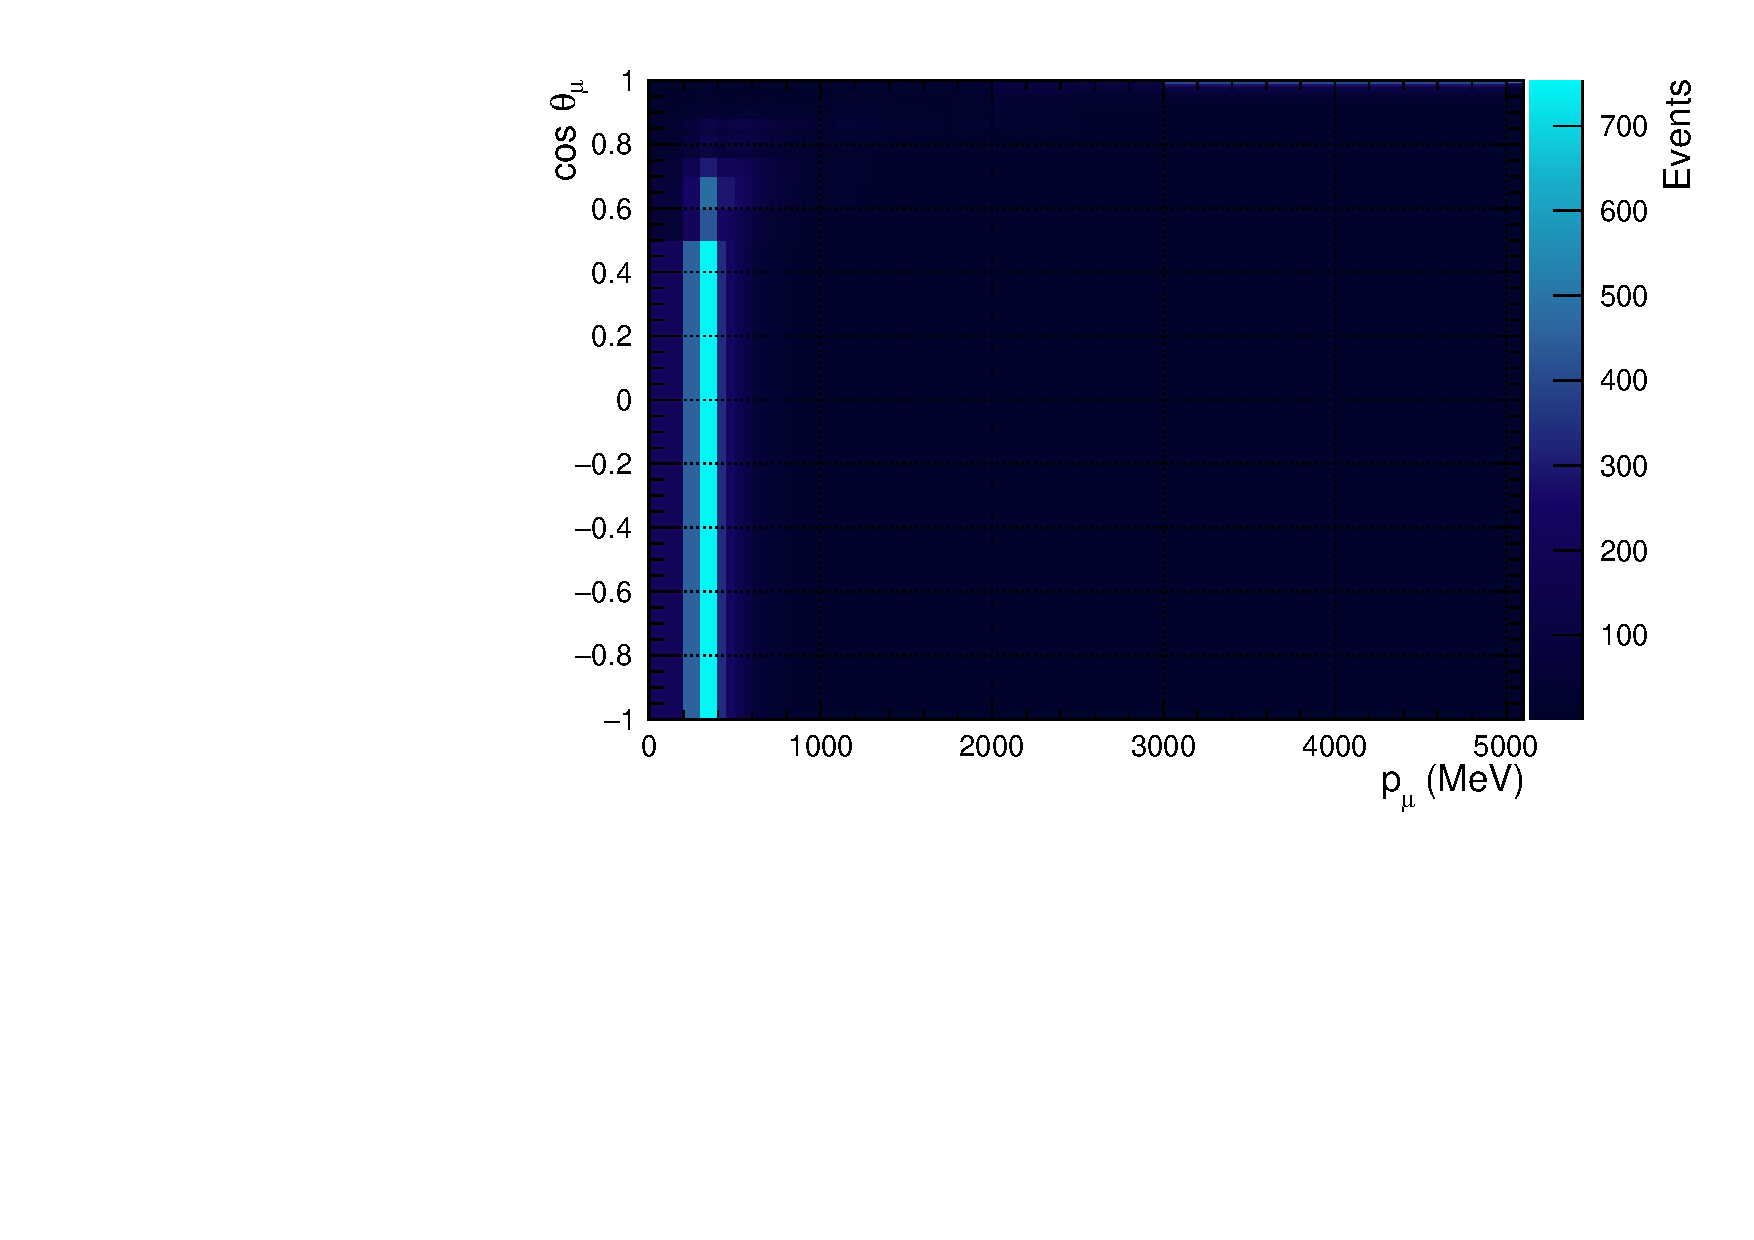
\includegraphics[width=0.95\linewidth]{figs/NomMC_MC_FGD1_numuCC_0pi}
  \caption{FGD1 FHC $\nu_{\mu}$ 0$\pi$}
  \label{fig:2d_FGD1_numuCC_0pi}
\end{subfigure}
\begin{subfigure}{.32\textwidth}
  \centering
  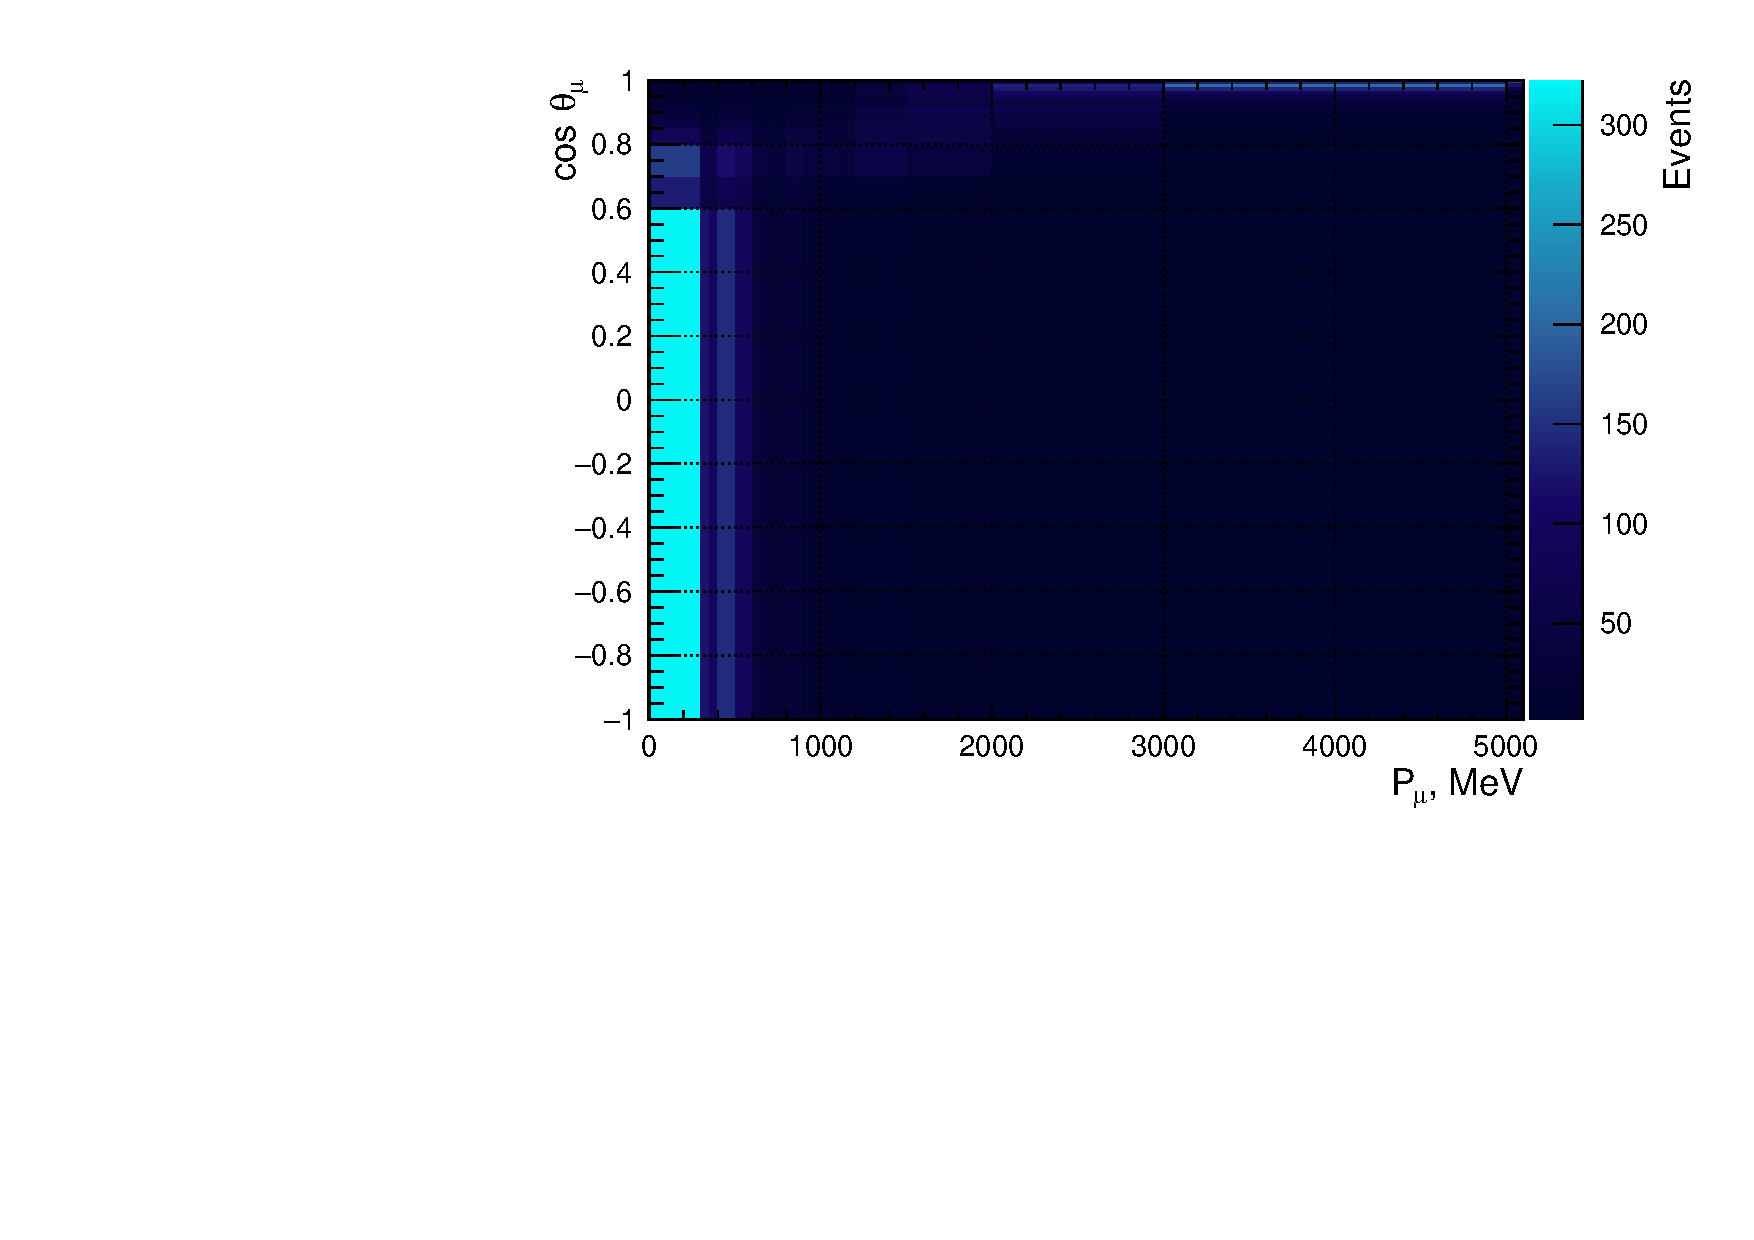
\includegraphics[width=0.95\linewidth]{figs/NomMC_MC_FGD1_numuCC_1pi}
  \caption{FGD1 FHC $\nu_{\mu}$ 1$\pi$}
  \label{fig:2d_FGD1_numuCC_1pi}
\end{subfigure}
\begin{subfigure}{.32\textwidth}
  \centering
  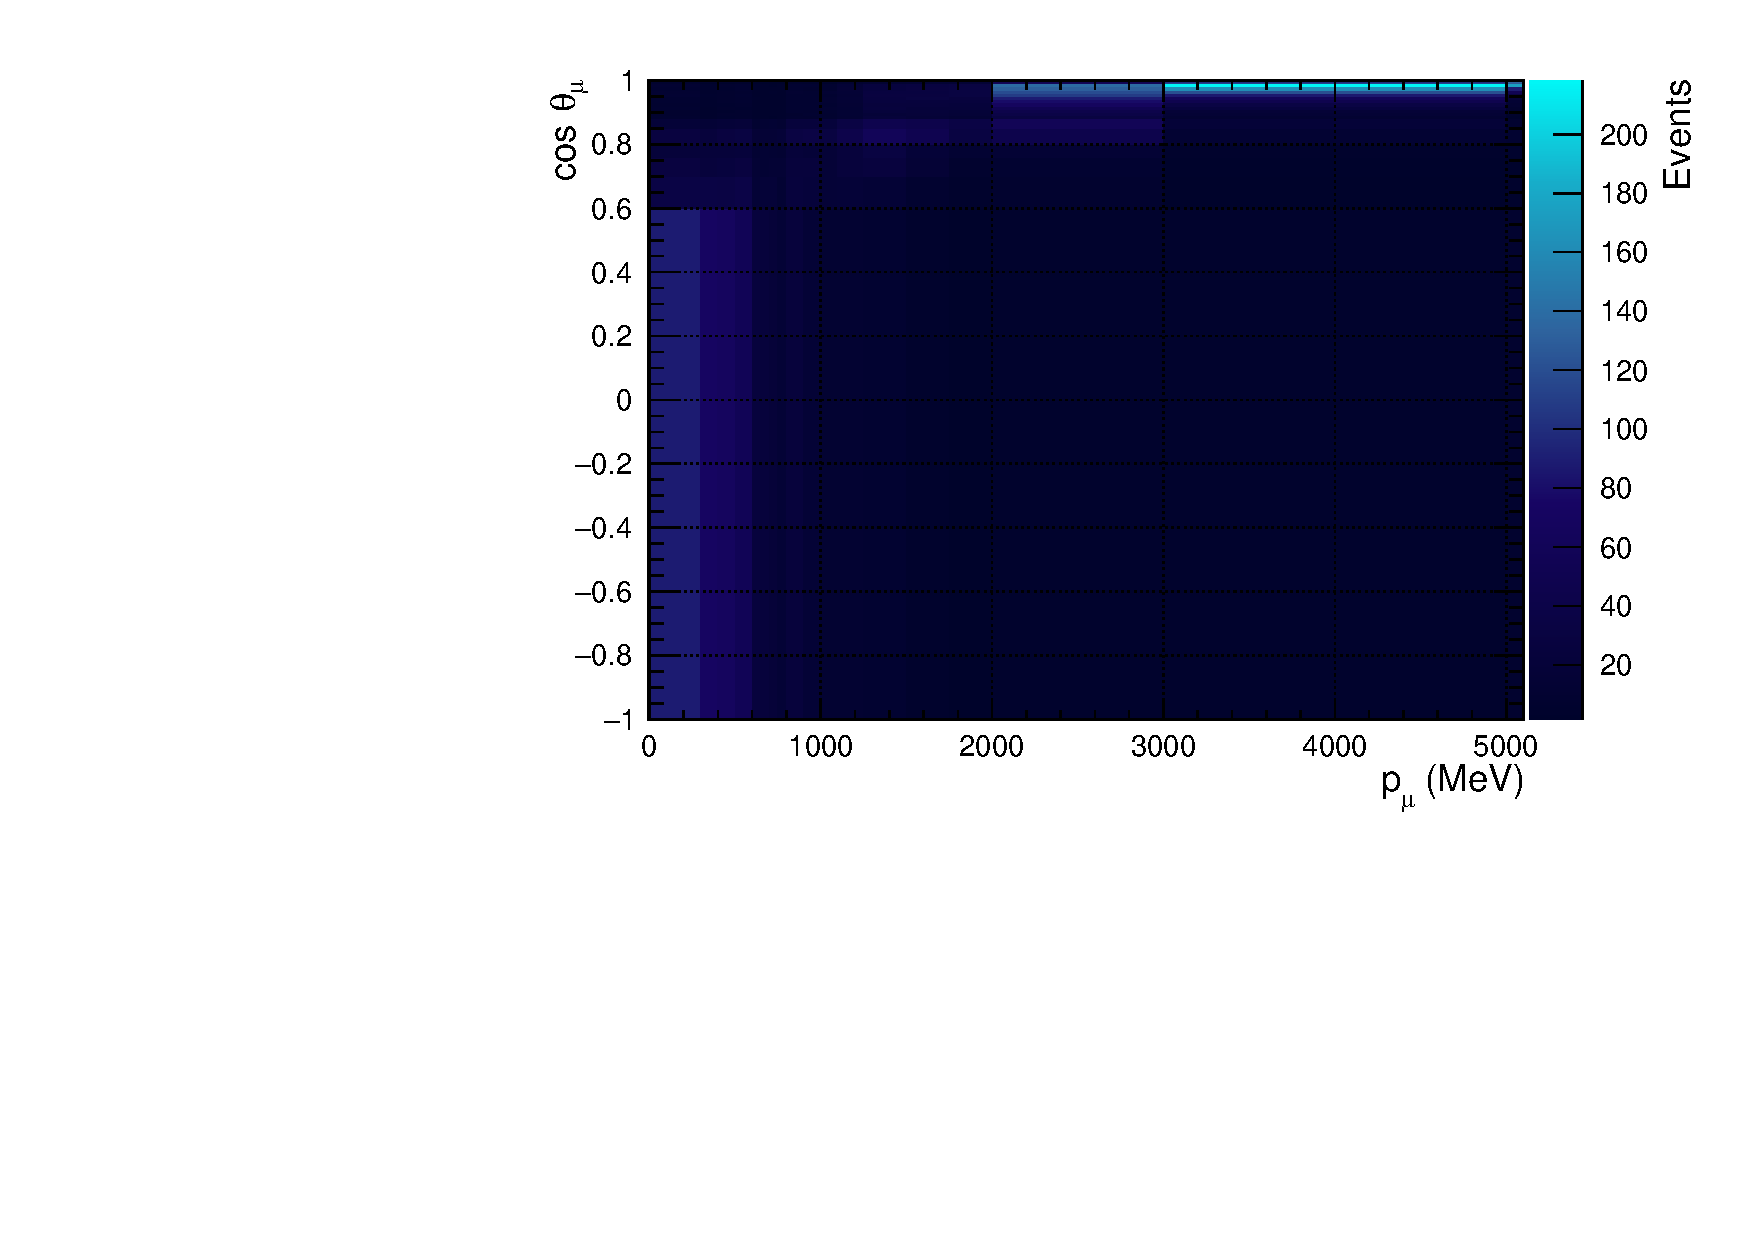
\includegraphics[width=0.95\linewidth]{figs/NomMC_MC_FGD1_numuCC_other}
  \caption{FGD1 FHC $\nu_{\mu}$ Other}
  \label{fig:2d_FGD1_numuCC_other}
\end{subfigure}
\centering
\begin{subfigure}{.32\textwidth}
  \centering
  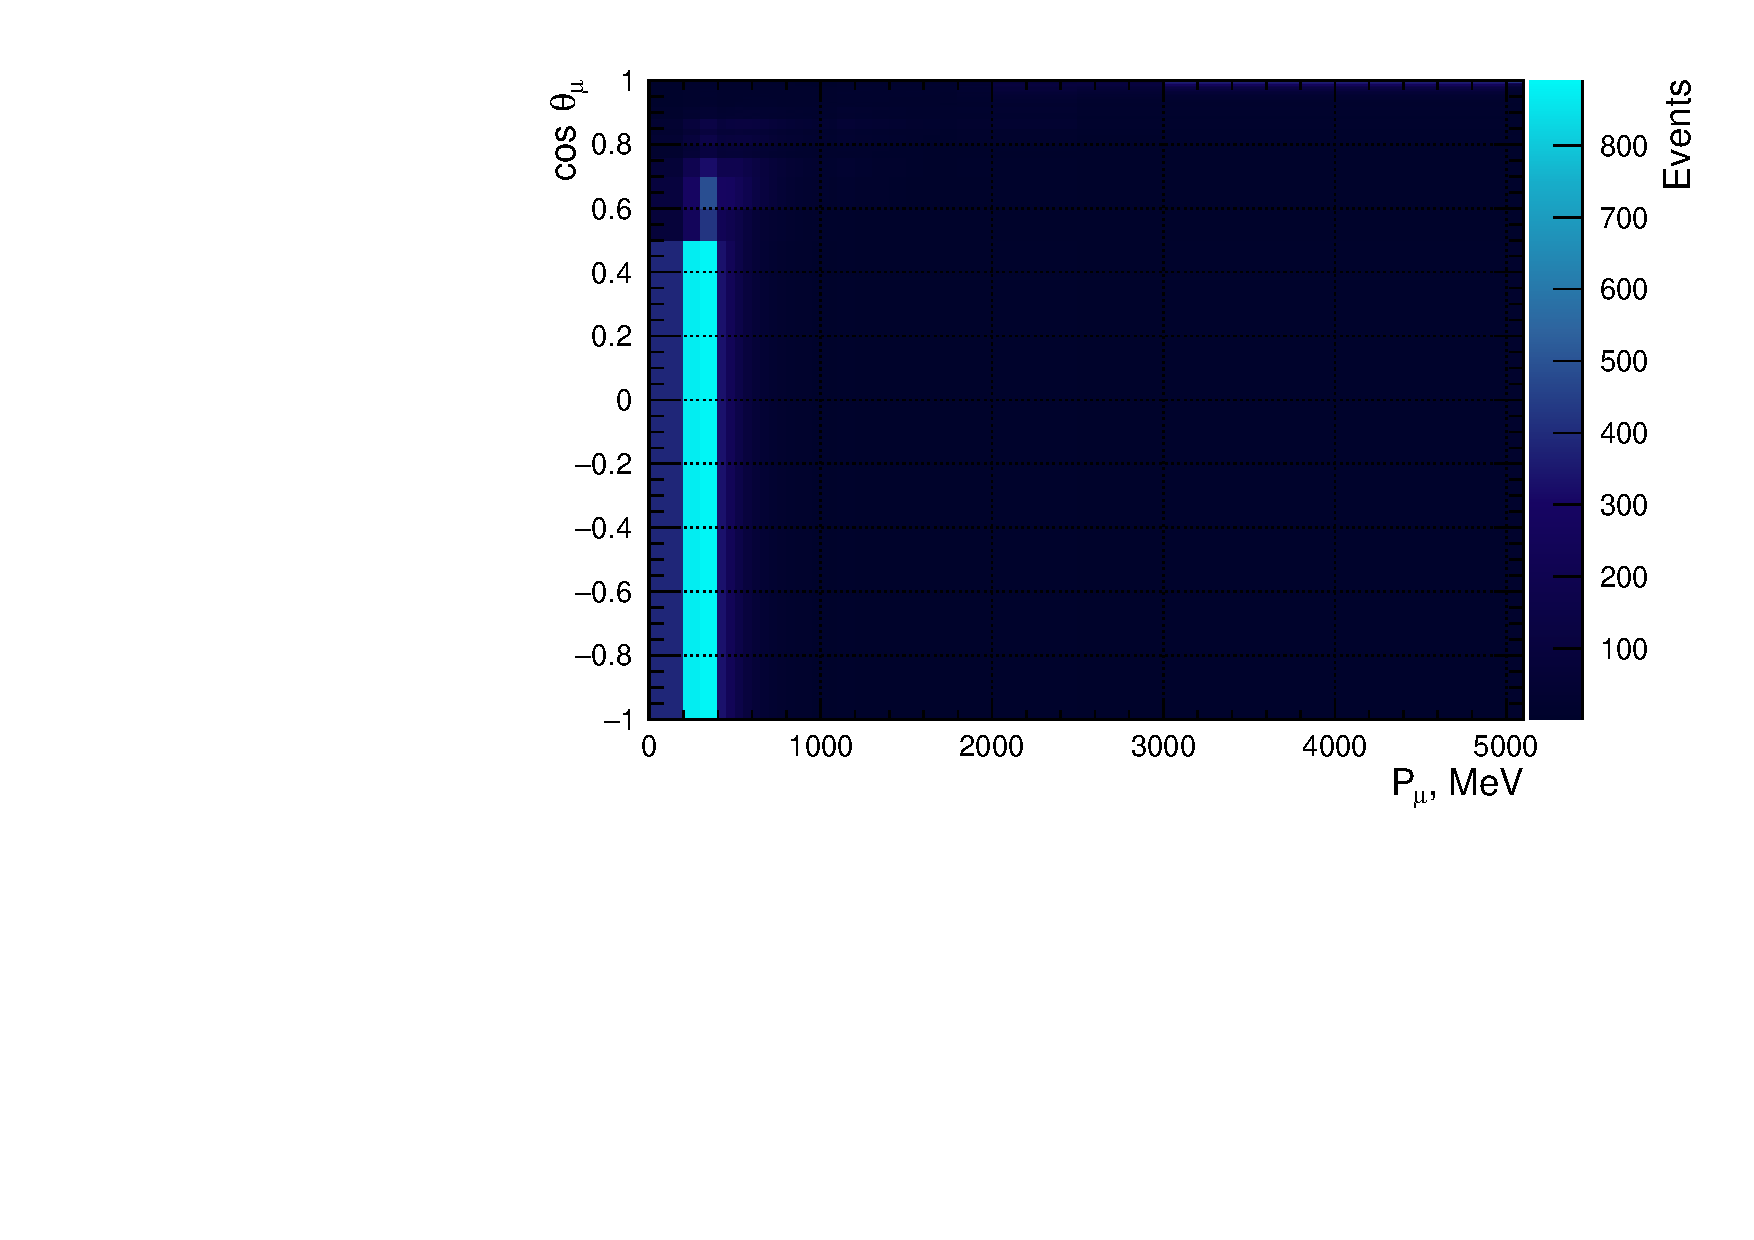
\includegraphics[width=0.95\linewidth]{figs/NomMC_MC_FGD2_numuCC_0pi}
  \caption{FGD2 FHC $\nu_{\mu}$ 0$\pi$}
  \label{fig:2d_FGD2_numuCC_0pi}
\end{subfigure}
\begin{subfigure}{.32\textwidth}
  \centering
  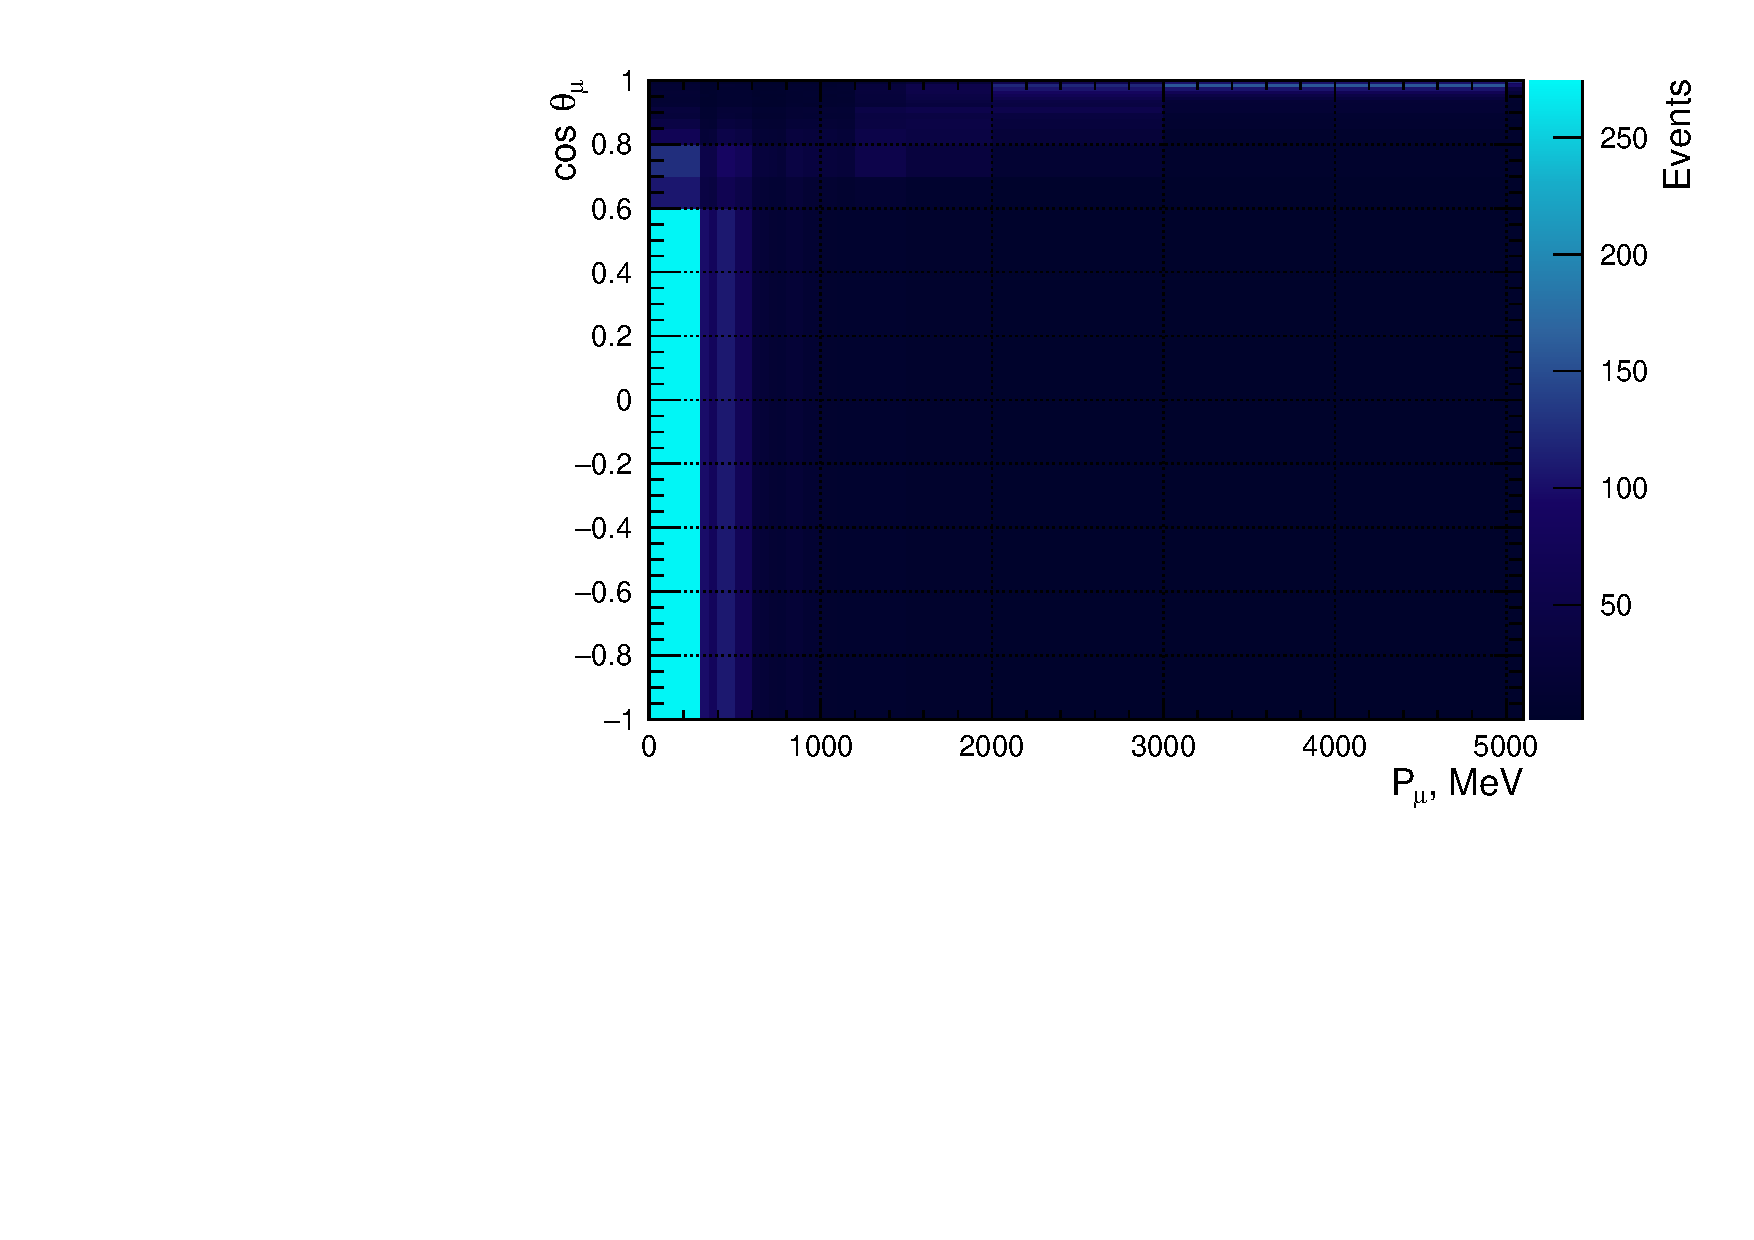
\includegraphics[width=0.95\linewidth]{figs/NomMC_MC_FGD2_numuCC_1pi}
  \caption{FGD2 FHC $\nu_{\mu}$ 1$\pi$}
  \label{fig:2d_FGD2_numuCC_1pi}
\end{subfigure}
\begin{subfigure}{.32\textwidth}
  \centering
  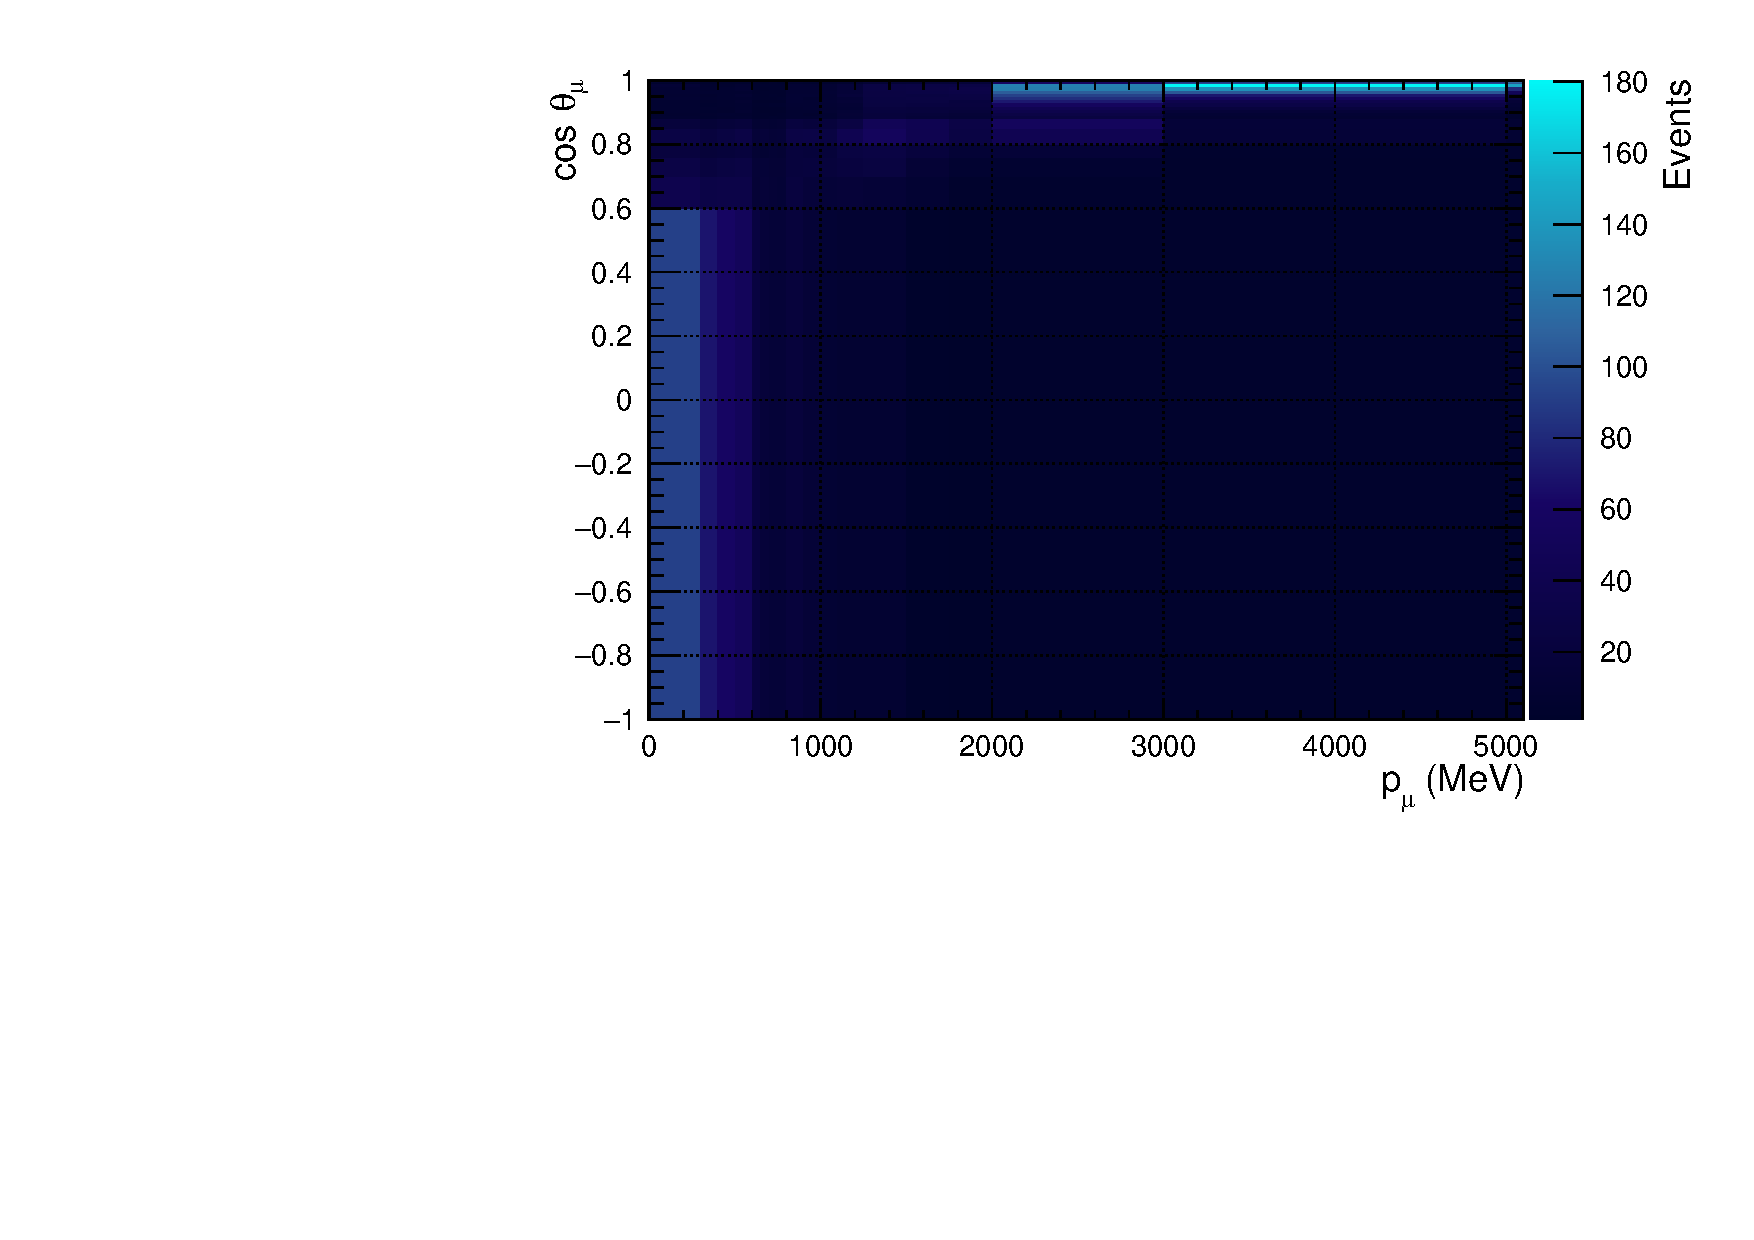
\includegraphics[width=0.95\linewidth]{figs/NomMC_MC_FGD2_numuCC_other}
  \caption{FGD2 $\nu_{\mu}$ Other}
  \label{fig:2d_FGD2_numuCC_other}
\end{subfigure}
\centering
\begin{subfigure}{.32\textwidth}
  \centering
  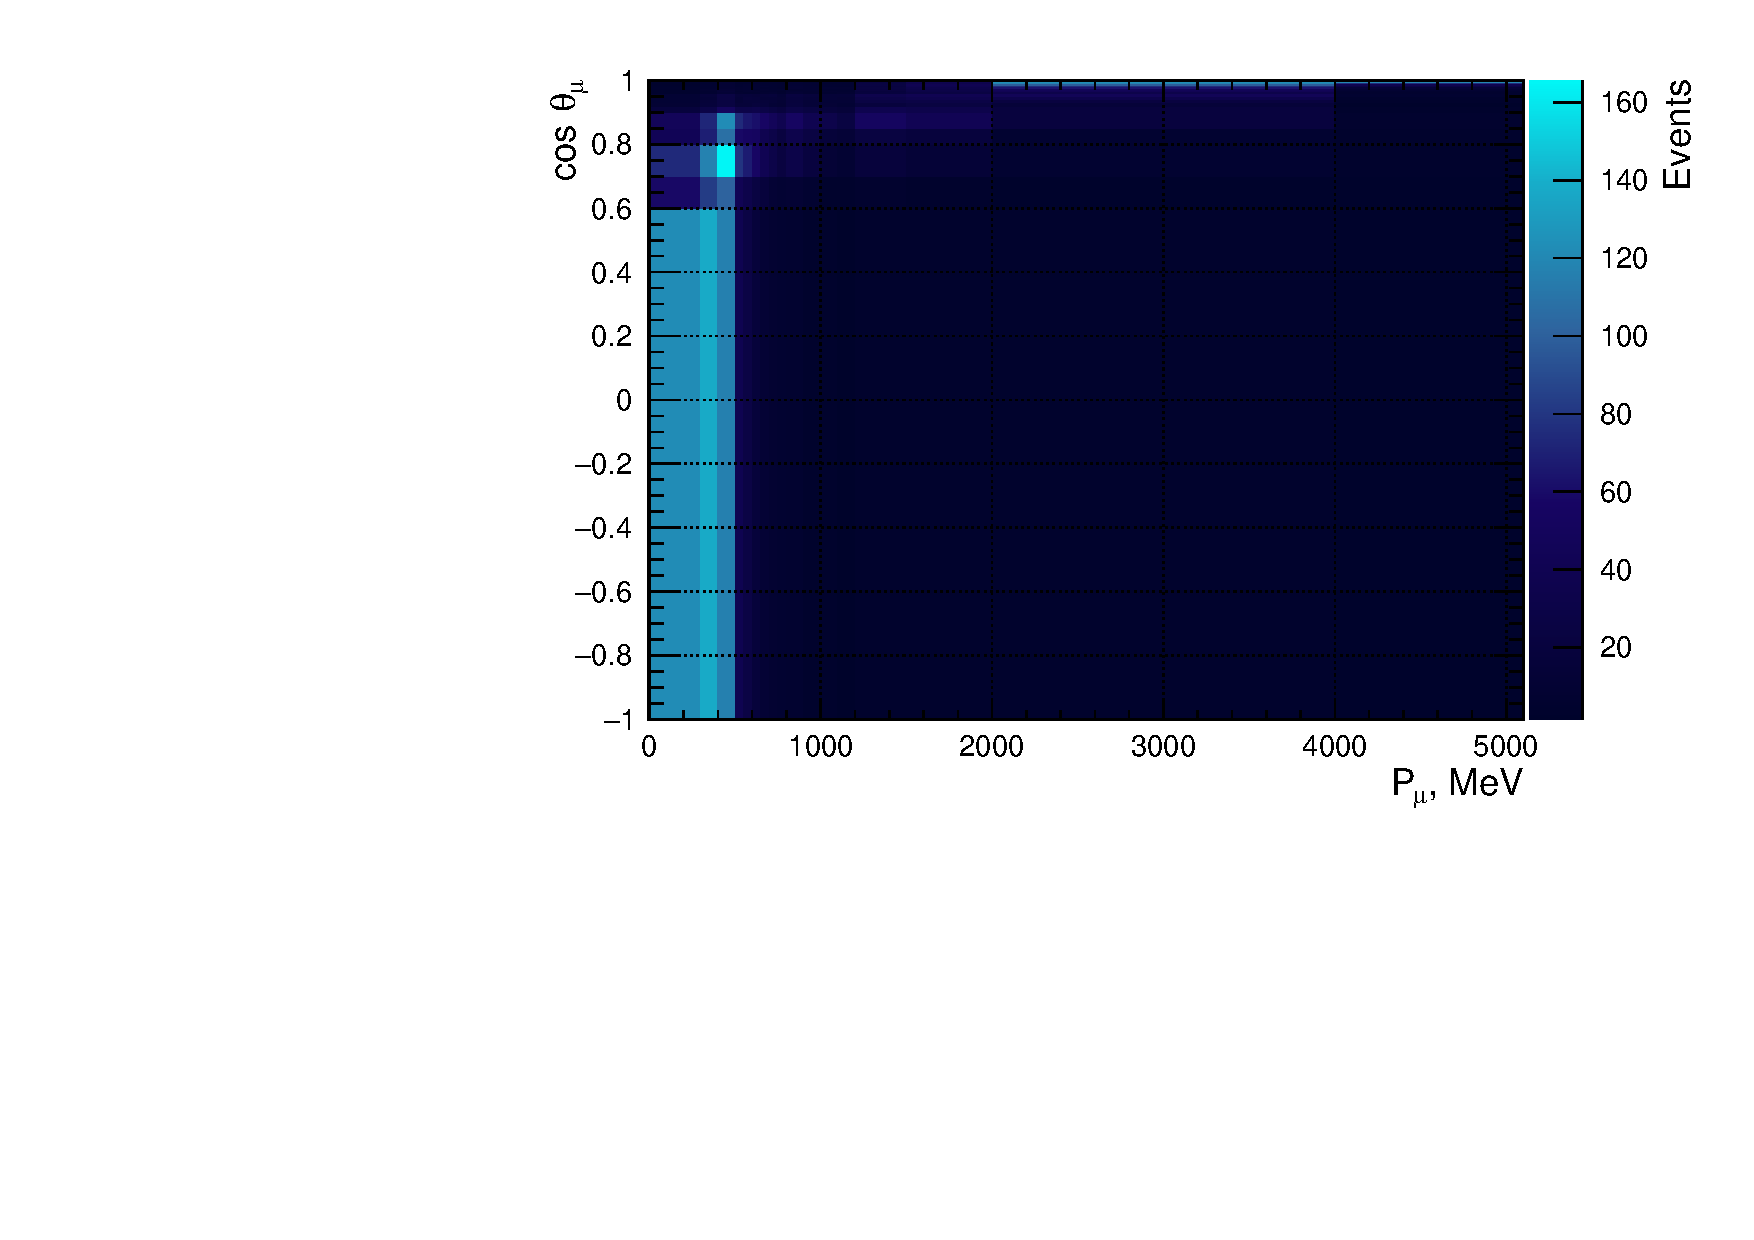
\includegraphics[width=0.95\linewidth]{figs/NomMC_MC_FGD1_anti-numuCC_0pi}
  \caption{FGD1 RHC $\bar{\nu_{\mu}}$ 0$\pi$}
  \label{fig:2d_FGD1_anti-numuCC_0pi}
\end{subfigure}
\begin{subfigure}{.32\textwidth}
  \centering
  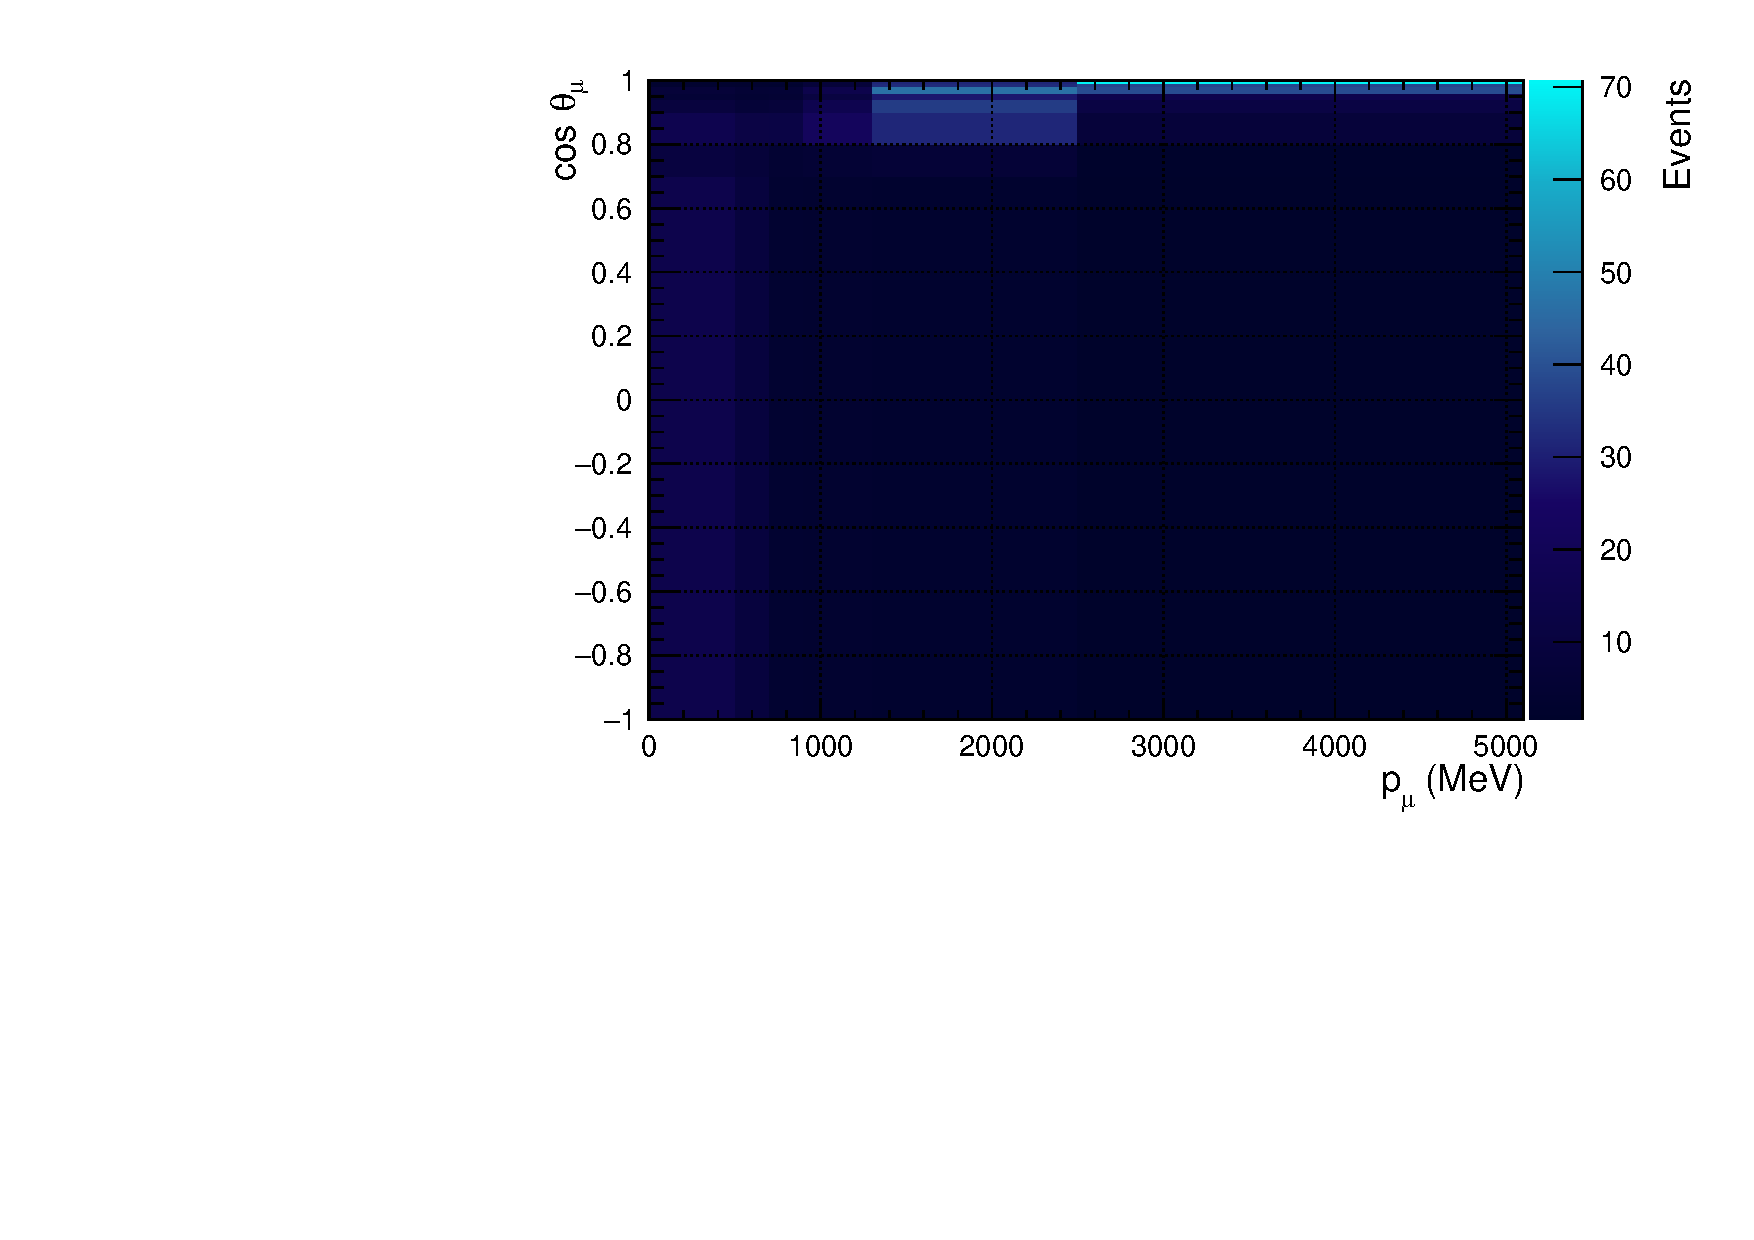
\includegraphics[width=0.95\linewidth]{figs/NomMC_MC_FGD1_anti-numuCC_1pi}
  \caption{FGD1 RHC $\bar{\nu_{\mu}}$ 1$\pi$}
  \label{fig:2d_FGD1_anti-numuCC_1pi}
\end{subfigure}
\begin{subfigure}{.32\textwidth}
  \centering
  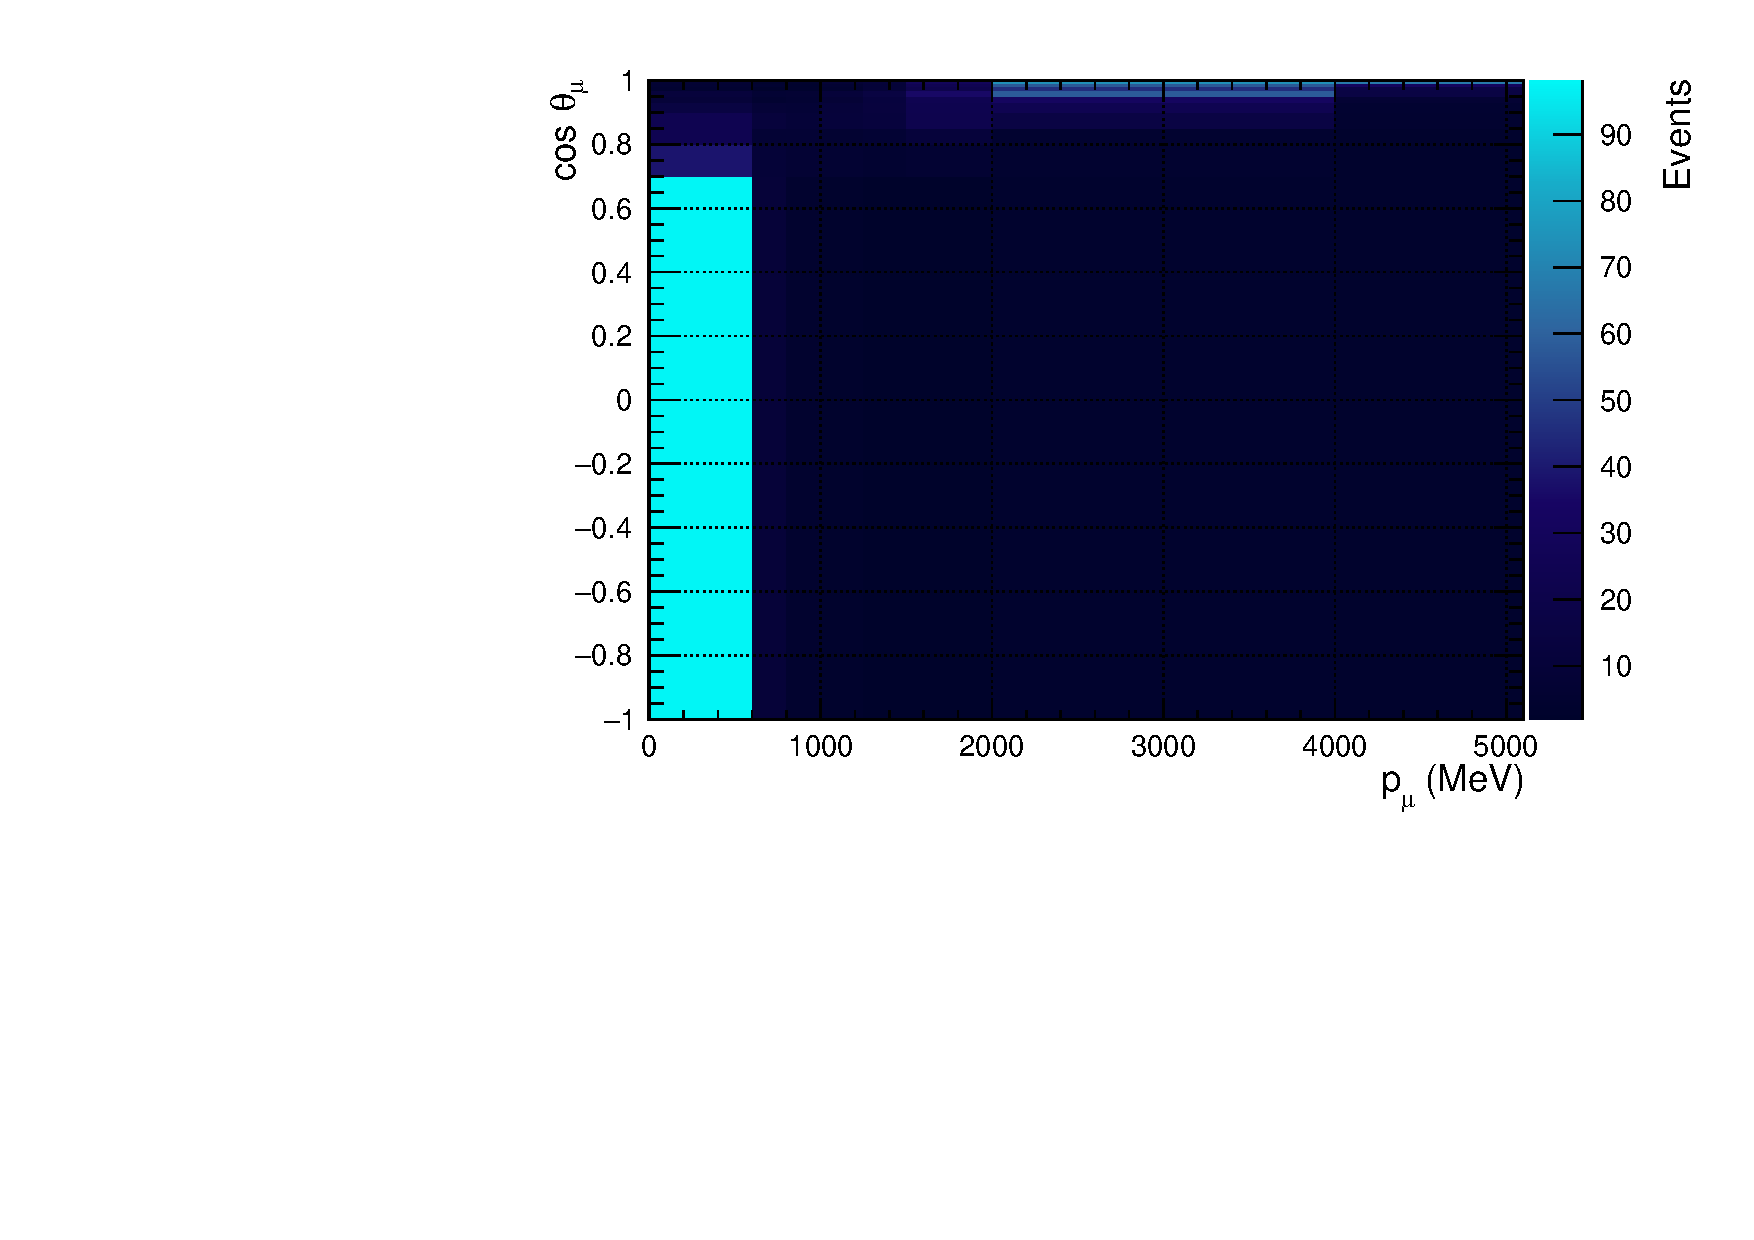
\includegraphics[width=0.95\linewidth]{figs/NomMC_MC_FGD1_anti-numuCC_other}
  \caption{FGD1 RHC $\bar{\nu_{\mu}}$ Other}
  \label{fig:2d_FGD1_anti-numuCC_other}
\end{subfigure}
\centering
\begin{subfigure}{.32\textwidth}
  \centering
  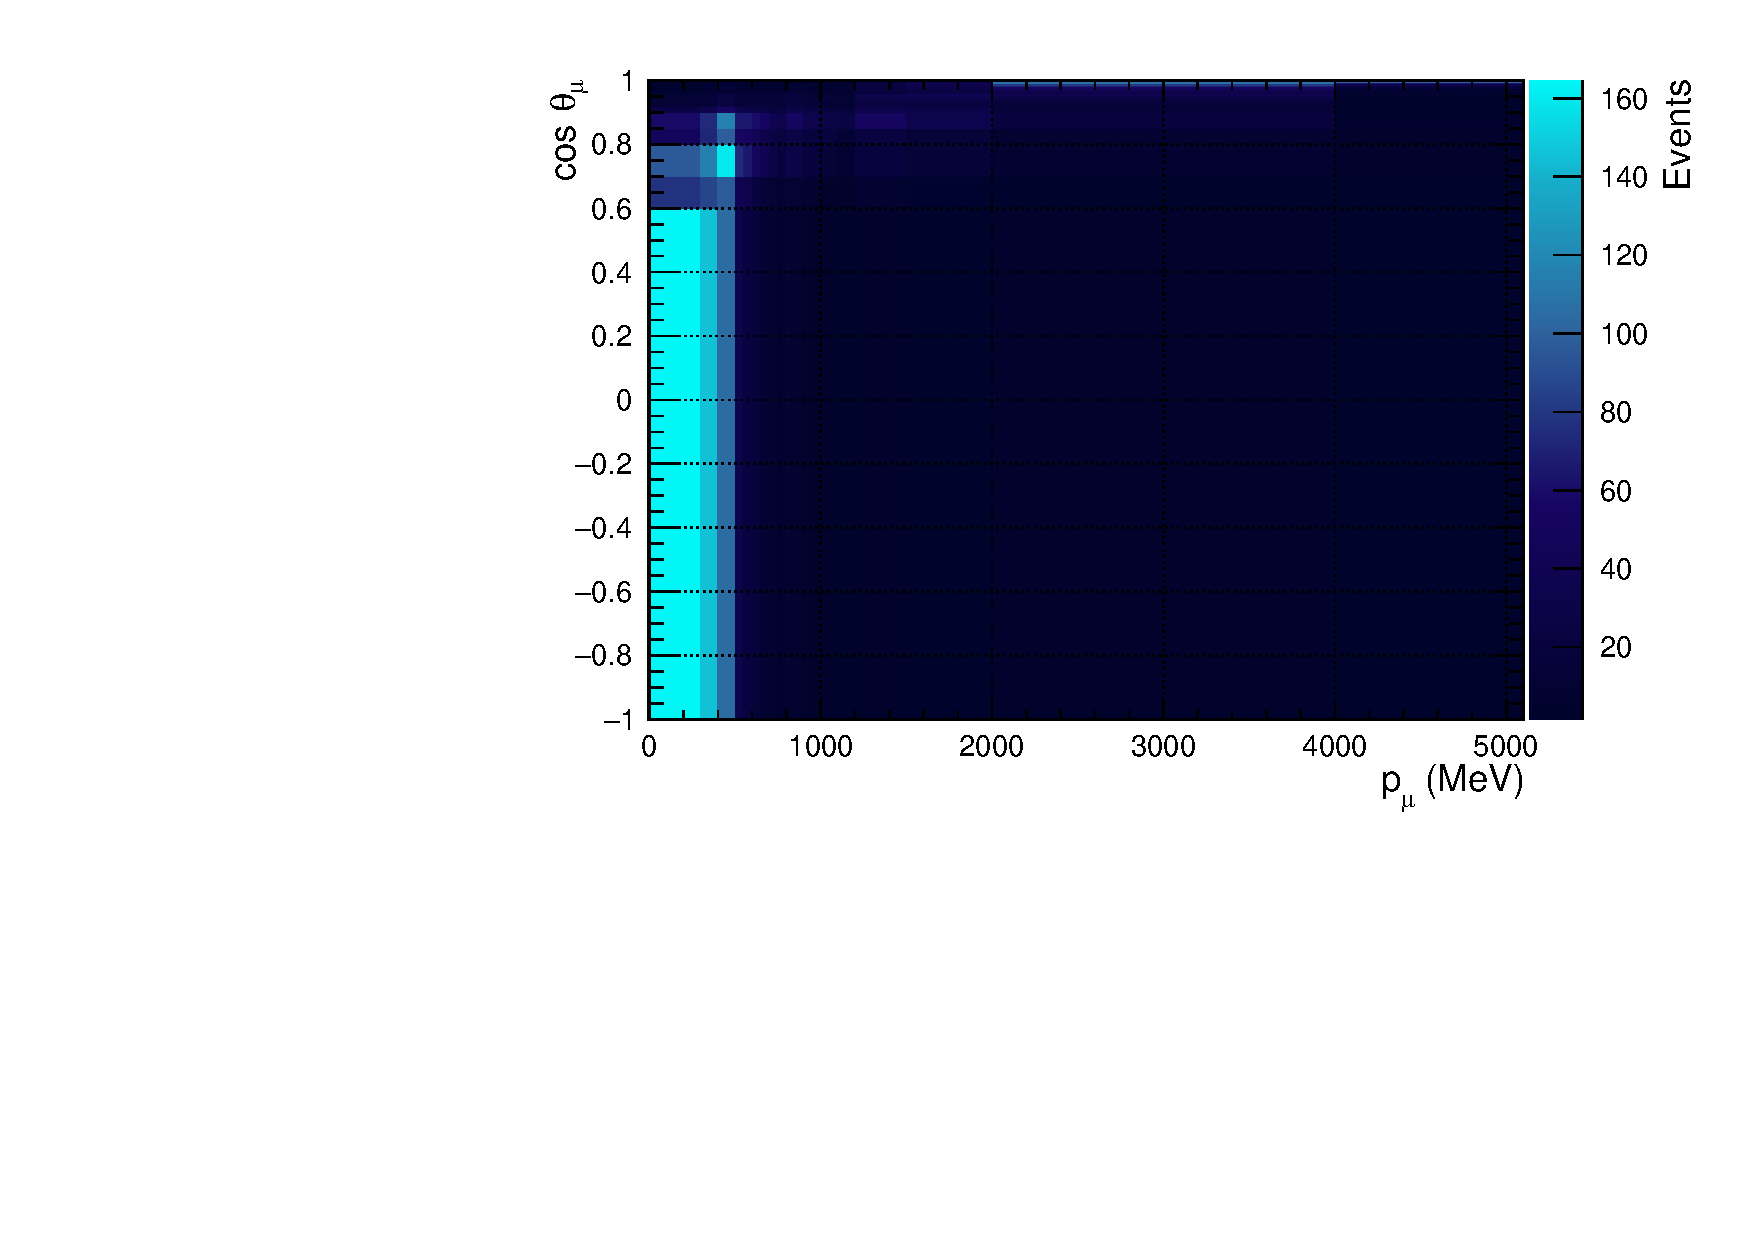
\includegraphics[width=0.95\linewidth]{figs/NomMC_MC_FGD2_anti-numuCC_0pi}
  \caption{FGD2 RHC $\bar{\nu_{\mu}}$ 0$\pi$}
  \label{fig:2d_FGD2_anti-numuCC_0pi}
\end{subfigure}
\begin{subfigure}{.32\textwidth}
  \centering
  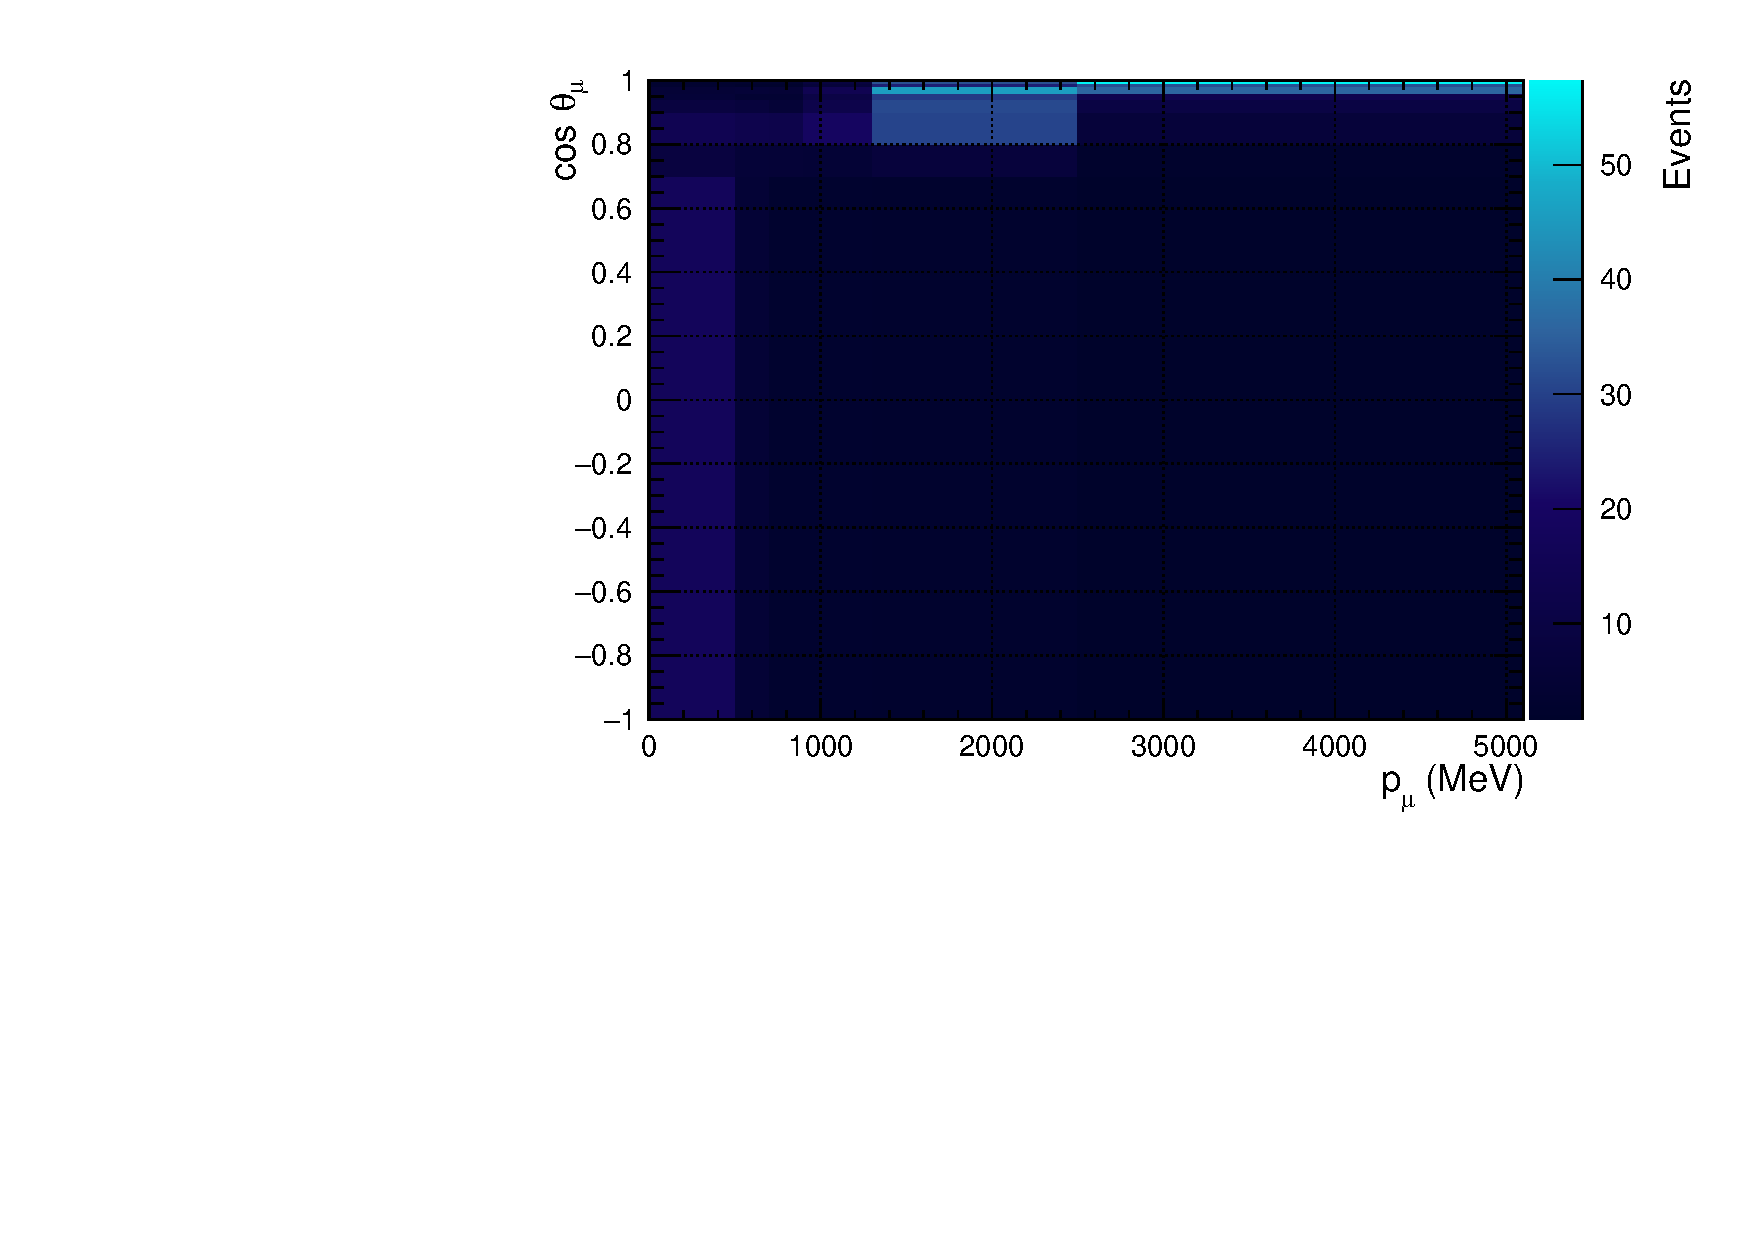
\includegraphics[width=0.95\linewidth]{figs/NomMC_MC_FGD2_anti-numuCC_1pi}
  \caption{FGD2 RHC $\bar{\nu_{\mu}}$ 1$\pi$}
  \label{fig:2d_FGD2_anti-numuCC_1pi}
\end{subfigure}
\begin{subfigure}{.32\textwidth}
  \centering
  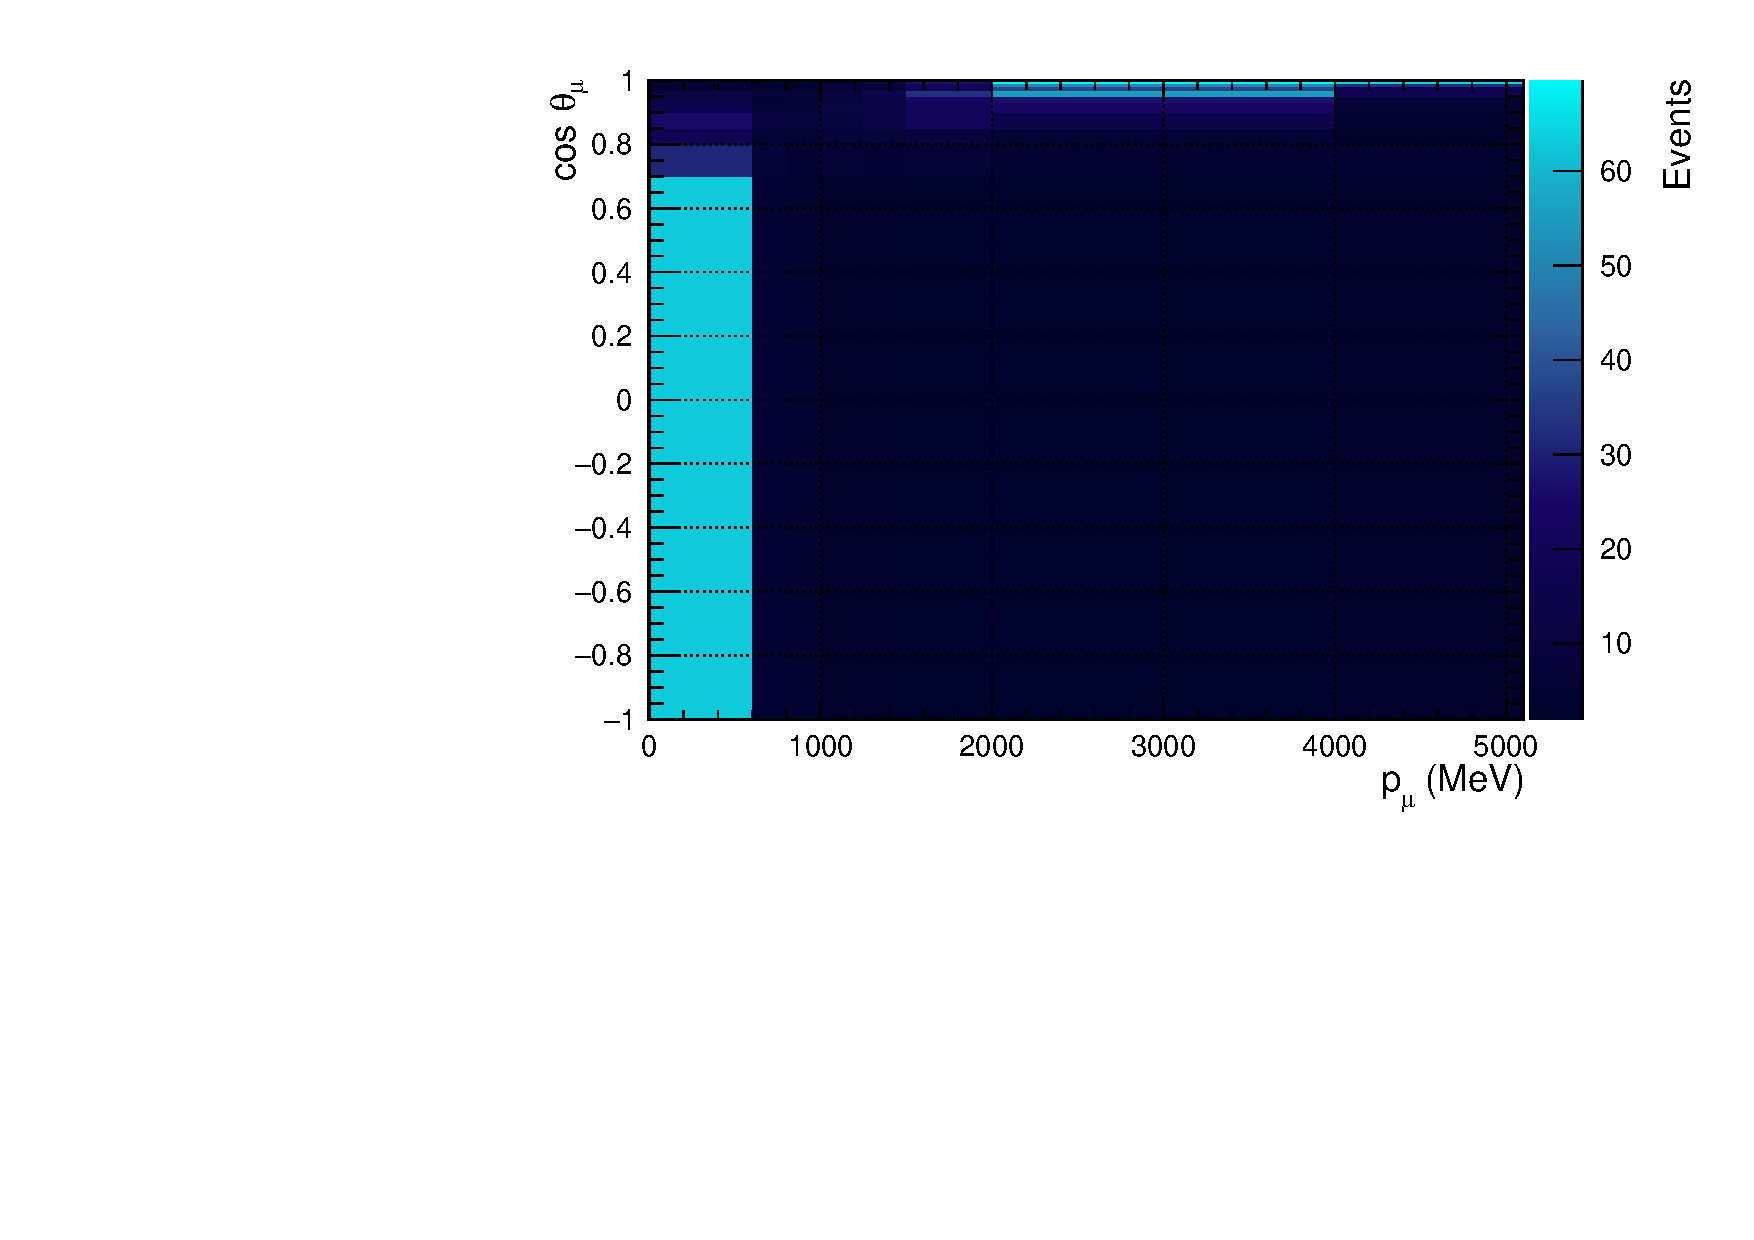
\includegraphics[width=0.95\linewidth]{figs/NomMC_MC_FGD2_anti-numuCC_other}
  \caption{FGD2 RHC $\bar{\nu_{\mu}}$ Other}
  \label{fig:2d_FGD2_anti-numuCC_other}
\end{subfigure}
\begin{subfigure}{.32\textwidth}
  \centering
  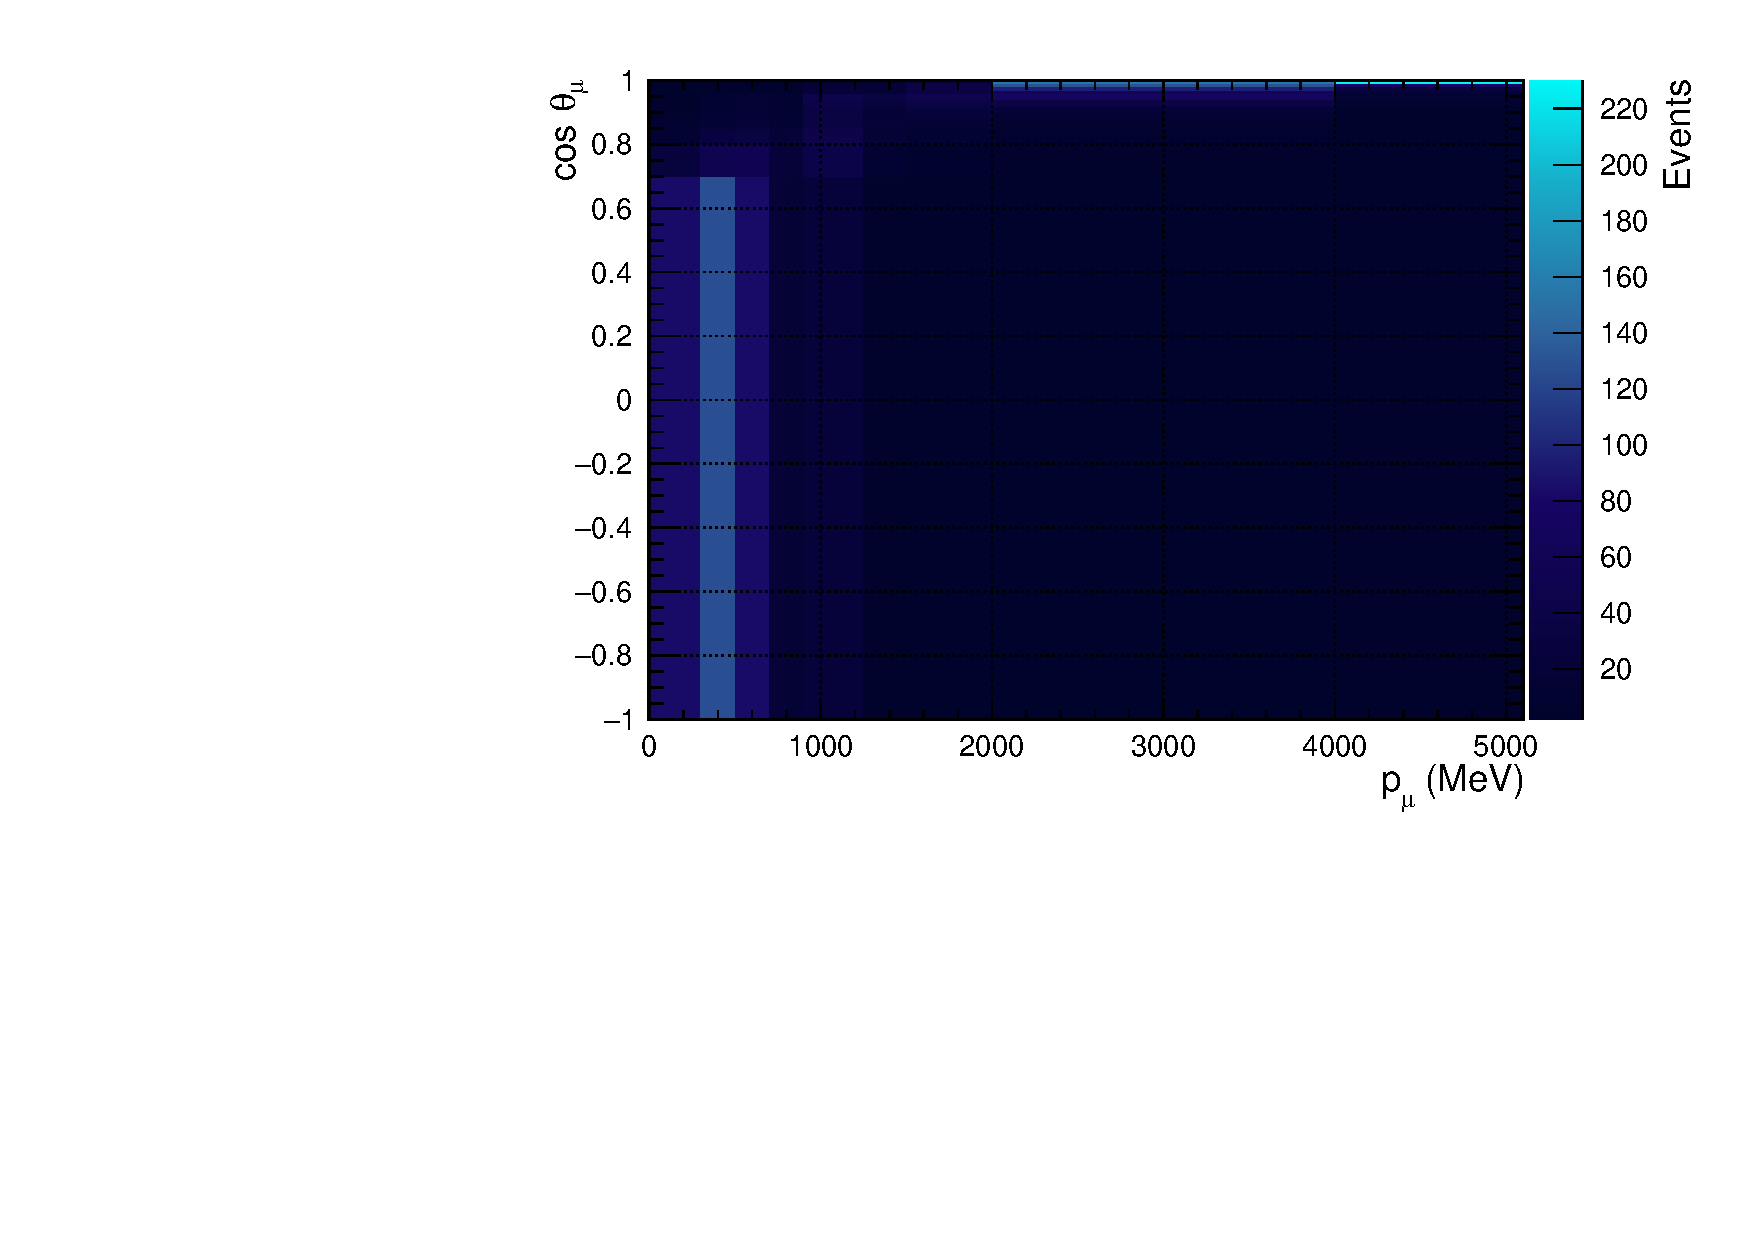
\includegraphics[width=0.95\linewidth]{figs/NomMC_MC_FGD1_NuMuBkg_CC0pi_in_AntiNu_Mode}
  \caption{FGD1 RHC $\nu_{\mu}$ 0$\pi$}
  \label{fig:2d_FGD1_NuMuBkg_CC0pi_in_AntiNu_Mode}
\end{subfigure}
\begin{subfigure}{.32\textwidth}
  \centering
  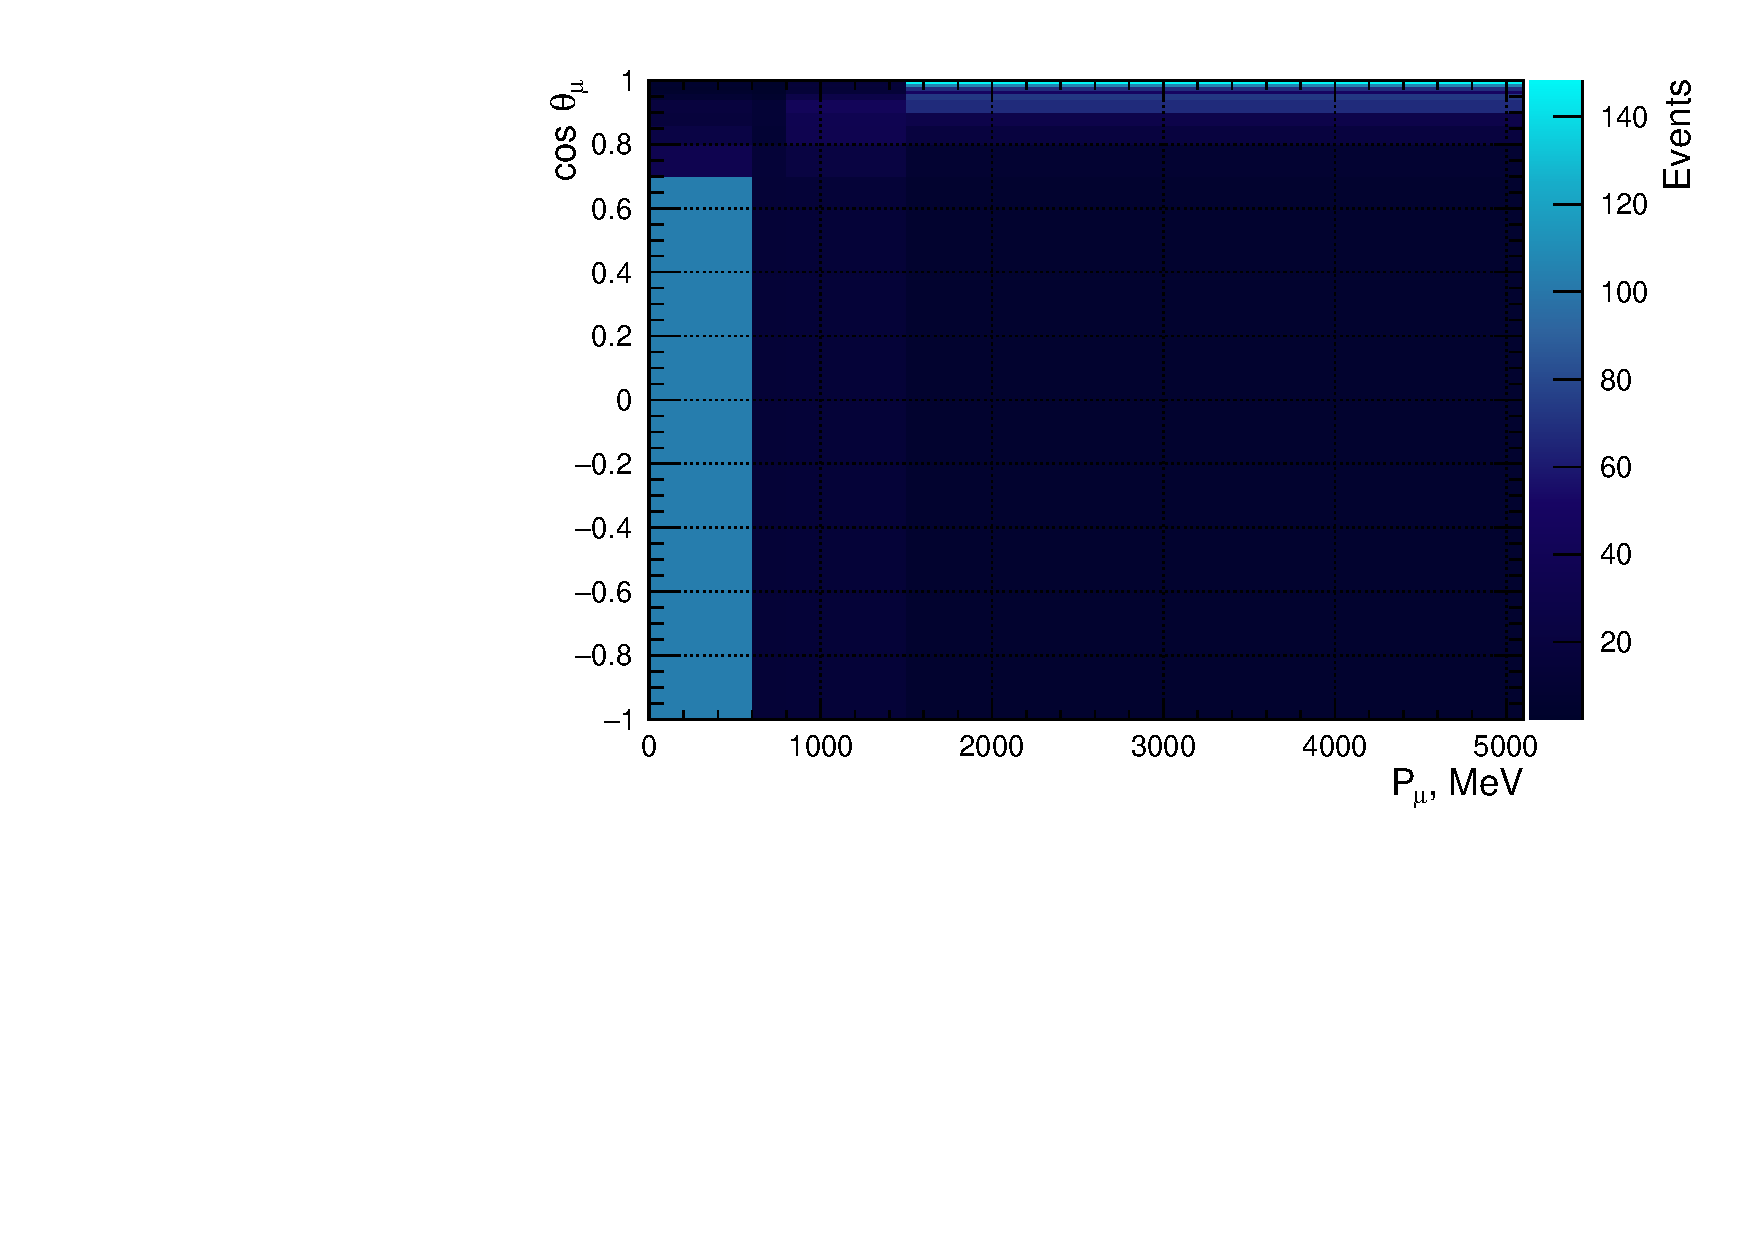
\includegraphics[width=0.95\linewidth]{figs/NomMC_MC_FGD1_NuMuBkg_CC1pi_in_AntiNu_Mode}
  \caption{FGD1 RHC $\nu_{\mu}$ 1$\pi$}
  \label{fig:2d_FGD1_NuMuBkg_CC1pi_in_AntiNu_Mode}
\end{subfigure}
\begin{subfigure}{.32\textwidth}
  \centering
  \includegraphics[width=0.95\linewidth]{figs/NomMC_MC_FGD1_NuMuBkg_CCOther_in_AntiNu_Mode}
  \caption{FGD1 RHC $\nu_{\mu}$ Other}
  \label{fig:2d_FGD1_NuMuBkg_CCOther_in_AntiNu_Mode}
\end{subfigure}
\begin{subfigure}{.32\textwidth}
  \centering
  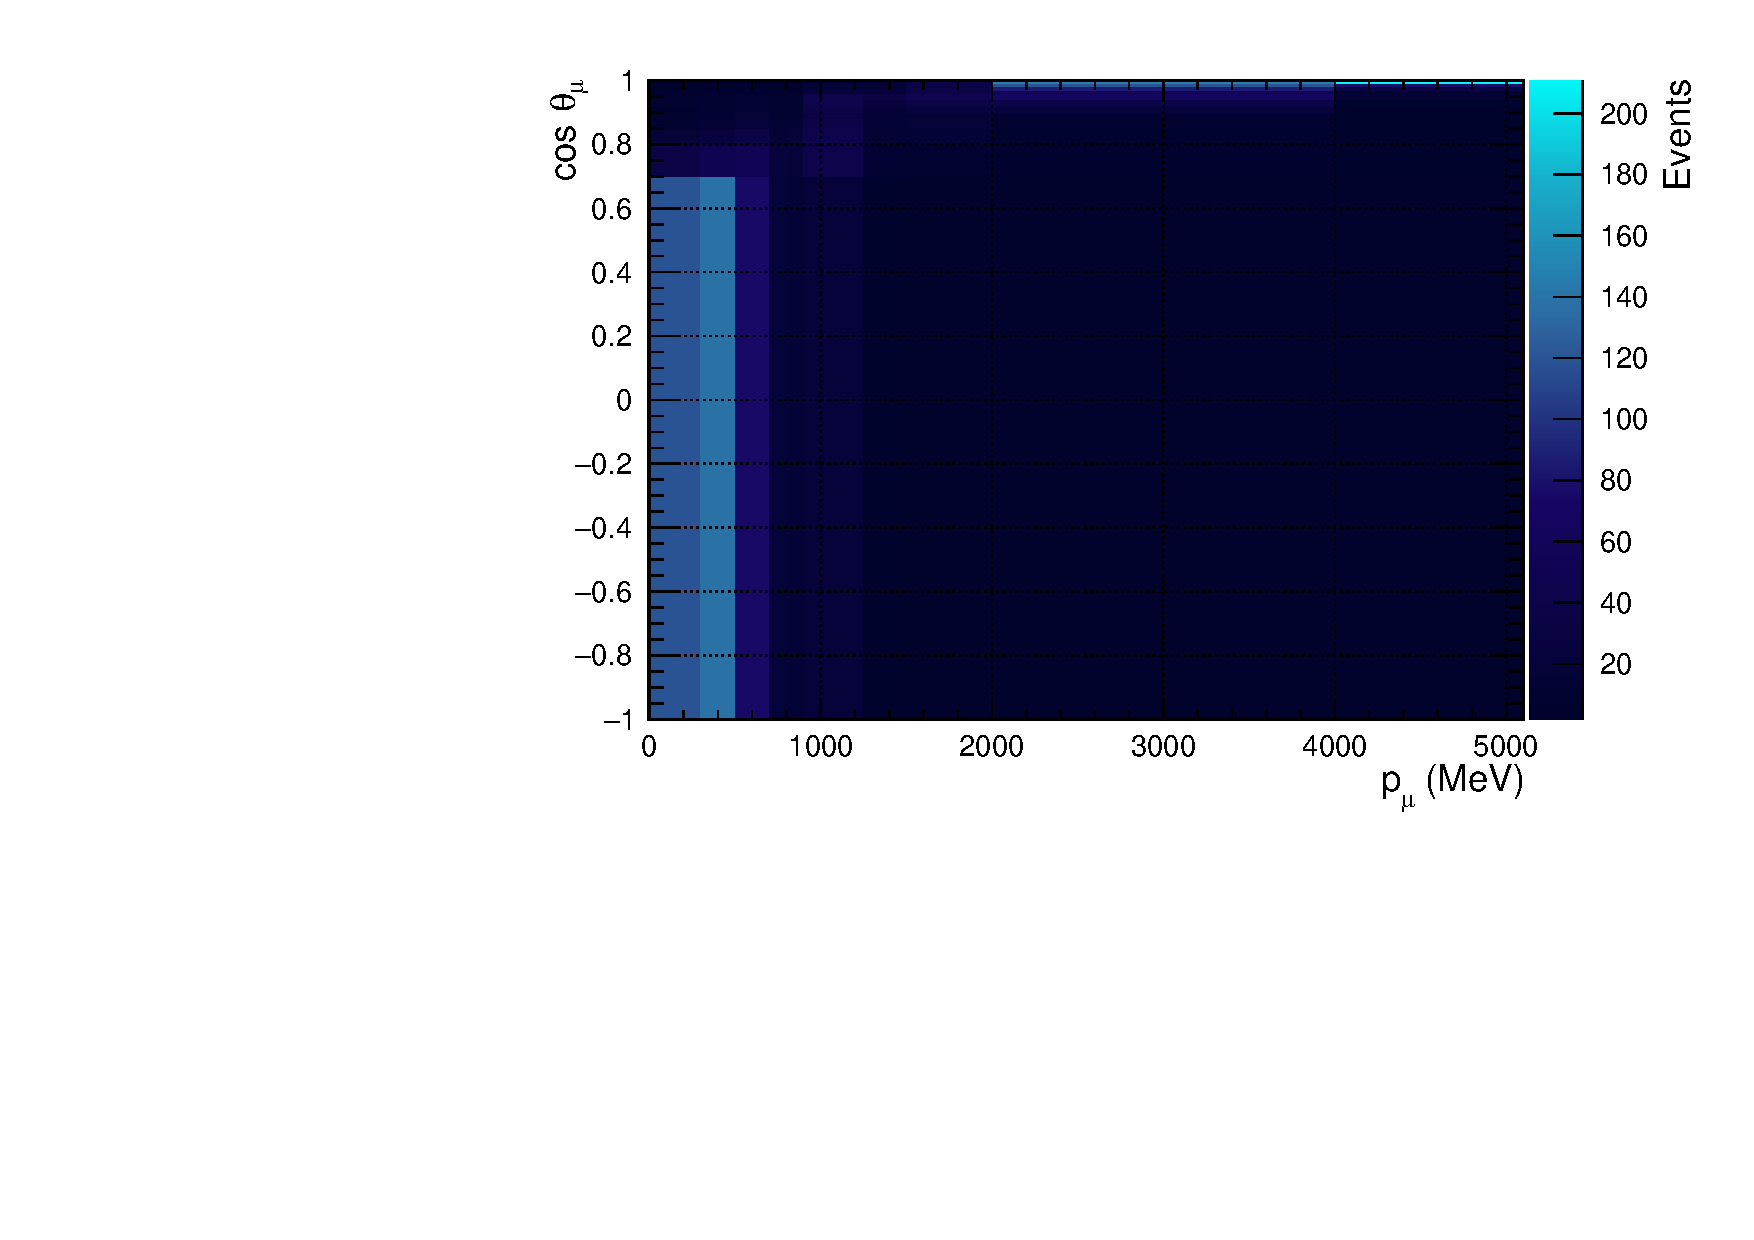
\includegraphics[width=0.95\linewidth]{figs/NomMC_MC_FGD2_NuMuBkg_CC0pi_in_AntiNu_Mode}
  \caption{FGD2 RHC $\nu_{\mu}$ 0$\pi$}
  \label{fig:2d_FGD2_NuMuBkg_CC0pi_in_AntiNu_Mode}
\end{subfigure}
\begin{subfigure}{.32\textwidth}
  \centering
  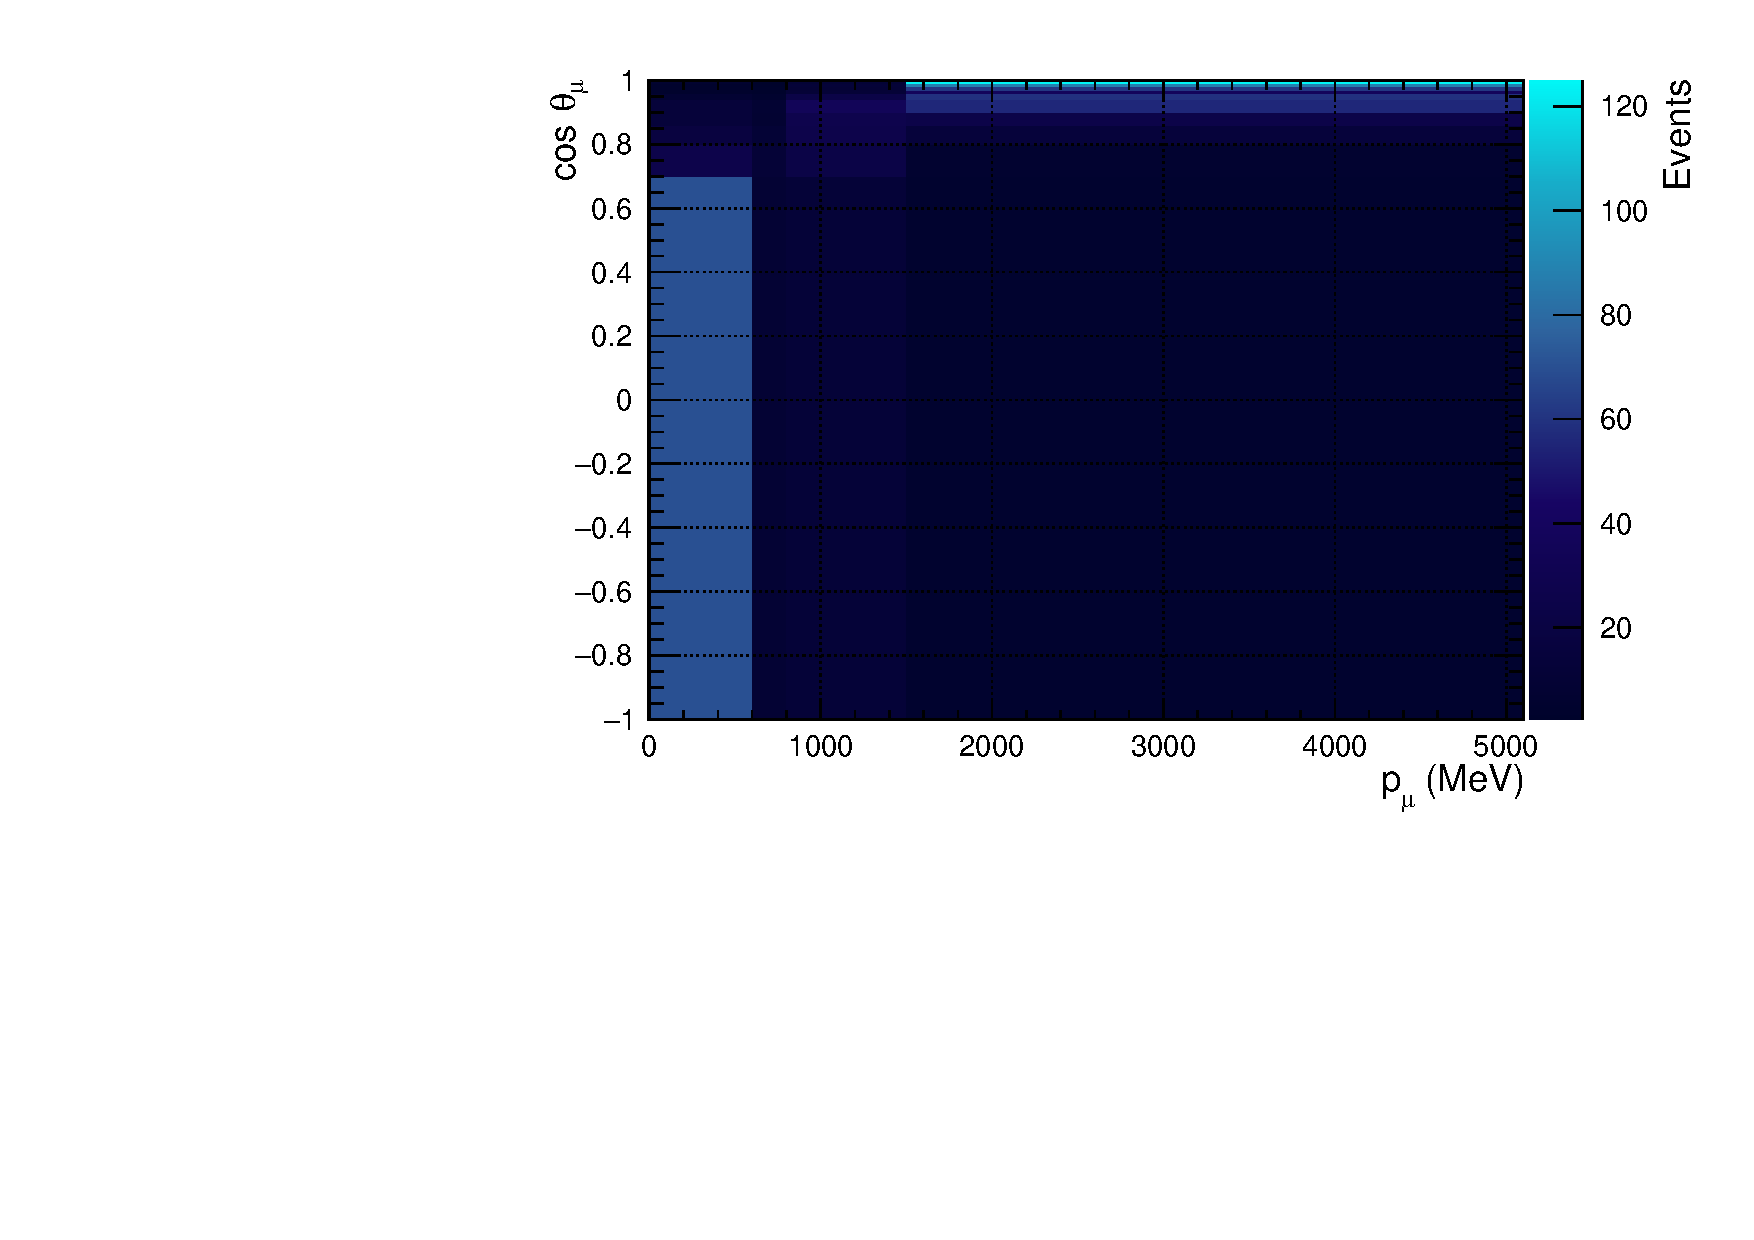
\includegraphics[width=0.95\linewidth]{figs/NomMC_MC_FGD2_NuMuBkg_CC1pi_in_AntiNu_Mode}
  \caption{FGD2 RHC $\nu_{\mu}$ 1$\pi$}
  \label{fig:2d_FGD2_NuMuBkg_CC1pi_in_AntiNu_Mode}
\end{subfigure}
\begin{subfigure}{.32\textwidth}
  \centering
  \includegraphics[width=0.95\linewidth]{figs/NomMC_MC_FGD2_NuMuBkg_CCOther_in_AntiNu_Mode}
  \caption{FGD2 RHC $\nu_{\mu}$ Other}
  \label{fig:2d_FGD2_NuMuBkg_CCOther_in_AntiNu_Mode}
\end{subfigure}
\caption{$p_{\mu}$-cos $\theta_{\mu}$ distributions for the nominal MC.}
\label{fig:2dnom}
\end{figure}

The projection of these distributions onto the $p_{\mu}$ axis are shown in Figure \ref{fig:pstack}, along with the data and interaction mode breakdown.

The CC 0$\pi$ and CC Other samples show oscillatory behaviour in the ratio of data to MC at low momentum. The ratio is consistently $>1$, but is slightly increased at the peak momentum for FHC and RHC $\nu$, and decreased at the peak for RHC $\bar{\nu}$. The ratio for the CC 1$\pi$ samples is more flat in momentum, but shows a small oscillation $<1$ at low momentum for FHC $\nu$, and $>1$ for RHC $\nu$ and $\bar{\nu}$. The behaviour is similar across the FGDs.

The FHC $\nu$ and RHC $\bar{\nu}$ CC 0$\pi$ samples are dominated by the target interaction modes CCQE and 2p2h. However, for RHC $\nu$, there is a large contamination of CC 1$\pi$ events. The FHC $\nu$ and RHC $\bar{\nu}$ CC 1$\pi$ samples are dominated by the target interaction modes CC 1$\pi$, CC coherent, and CC mult-$\pi$. For RHC $\nu$ the 1$\pi$ sample has a significant number of CC DIS events. The CC Other samples are populated by mainly the target interaction modes CC DIS, CC mult-$\pi$, and CC miscellaneous, but with a significant number CC $1\pi$ and CC coherent events for FHC $\nu$ and RHC $\bar{\nu}$.

\begin{figure}
\centering
\begin{subfigure}{.35\textwidth}
  \centering
  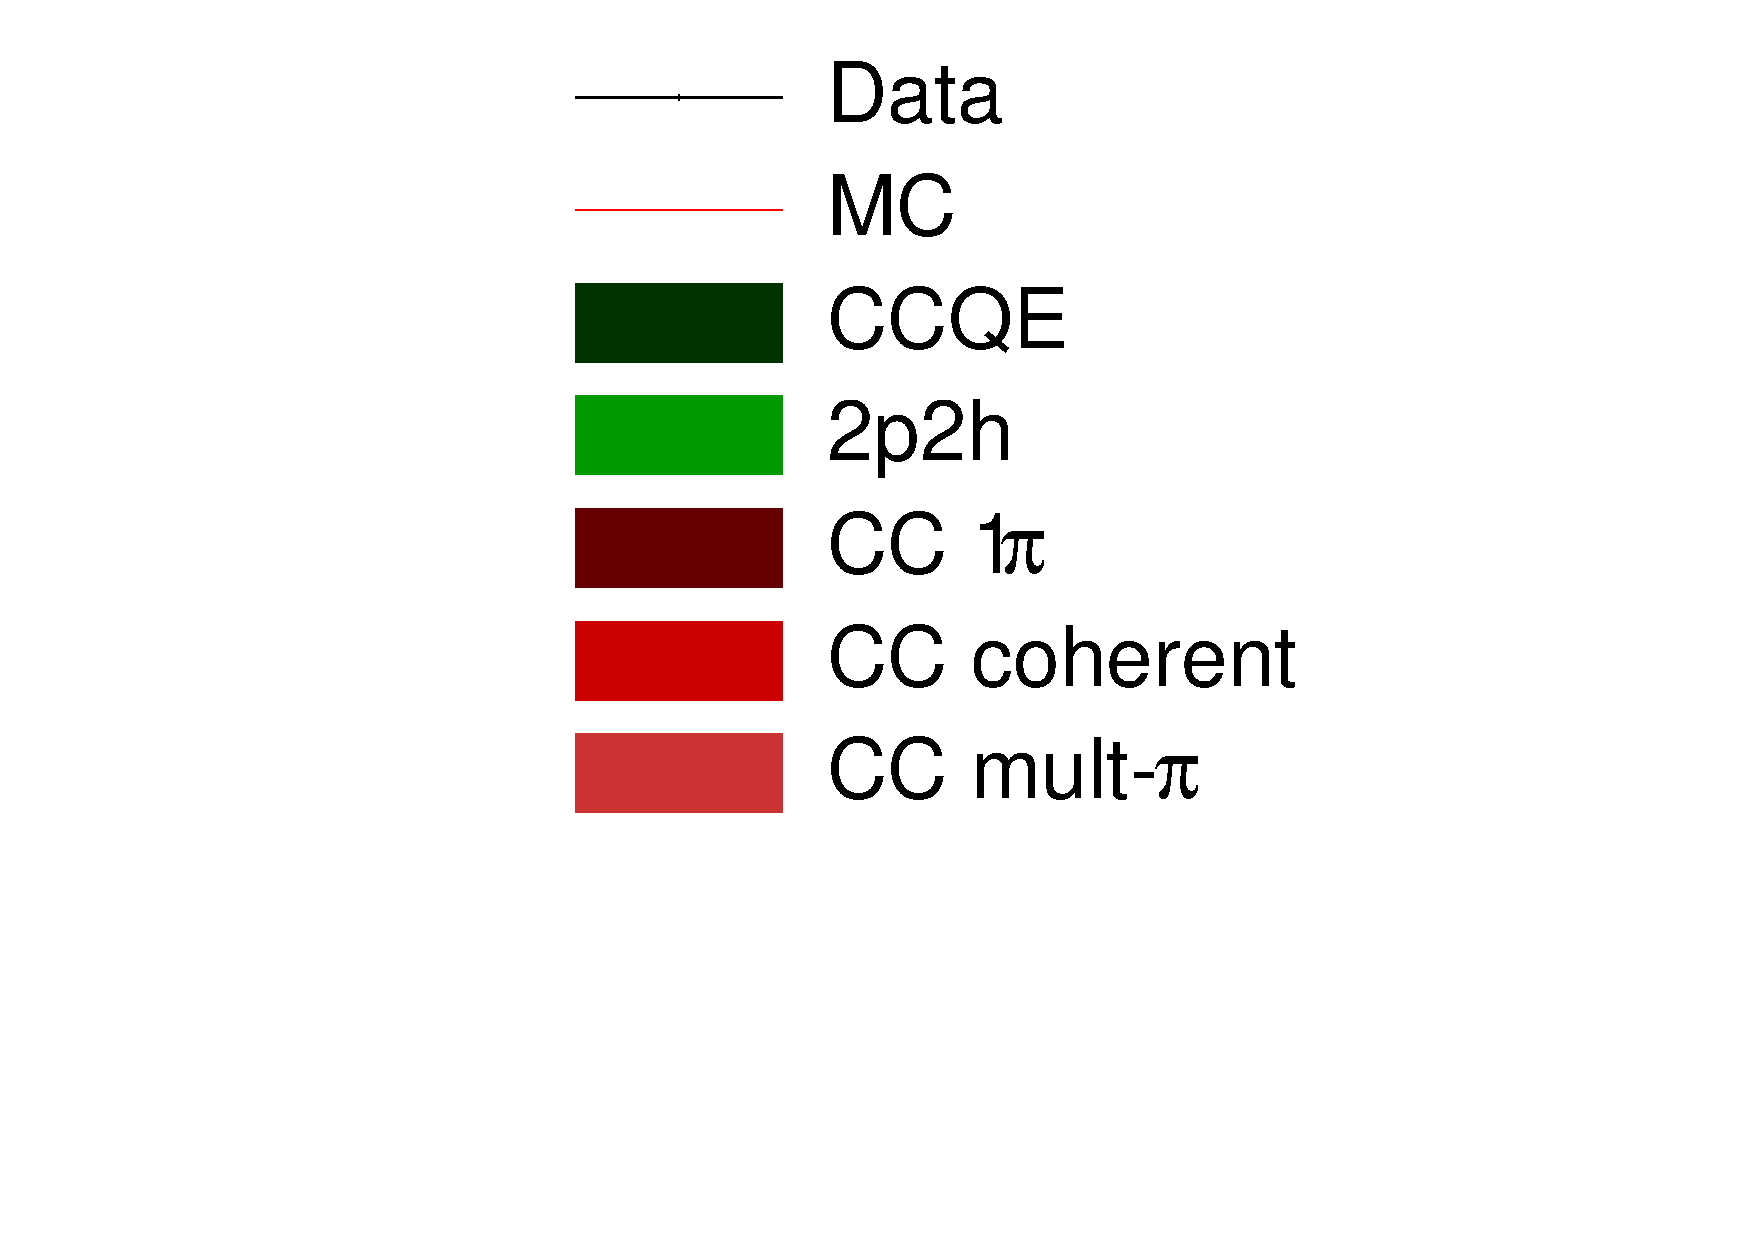
\includegraphics[width=0.7\linewidth]{figs/legend}
\end{subfigure}
\begin{subfigure}{.35\textwidth}
  \centering
  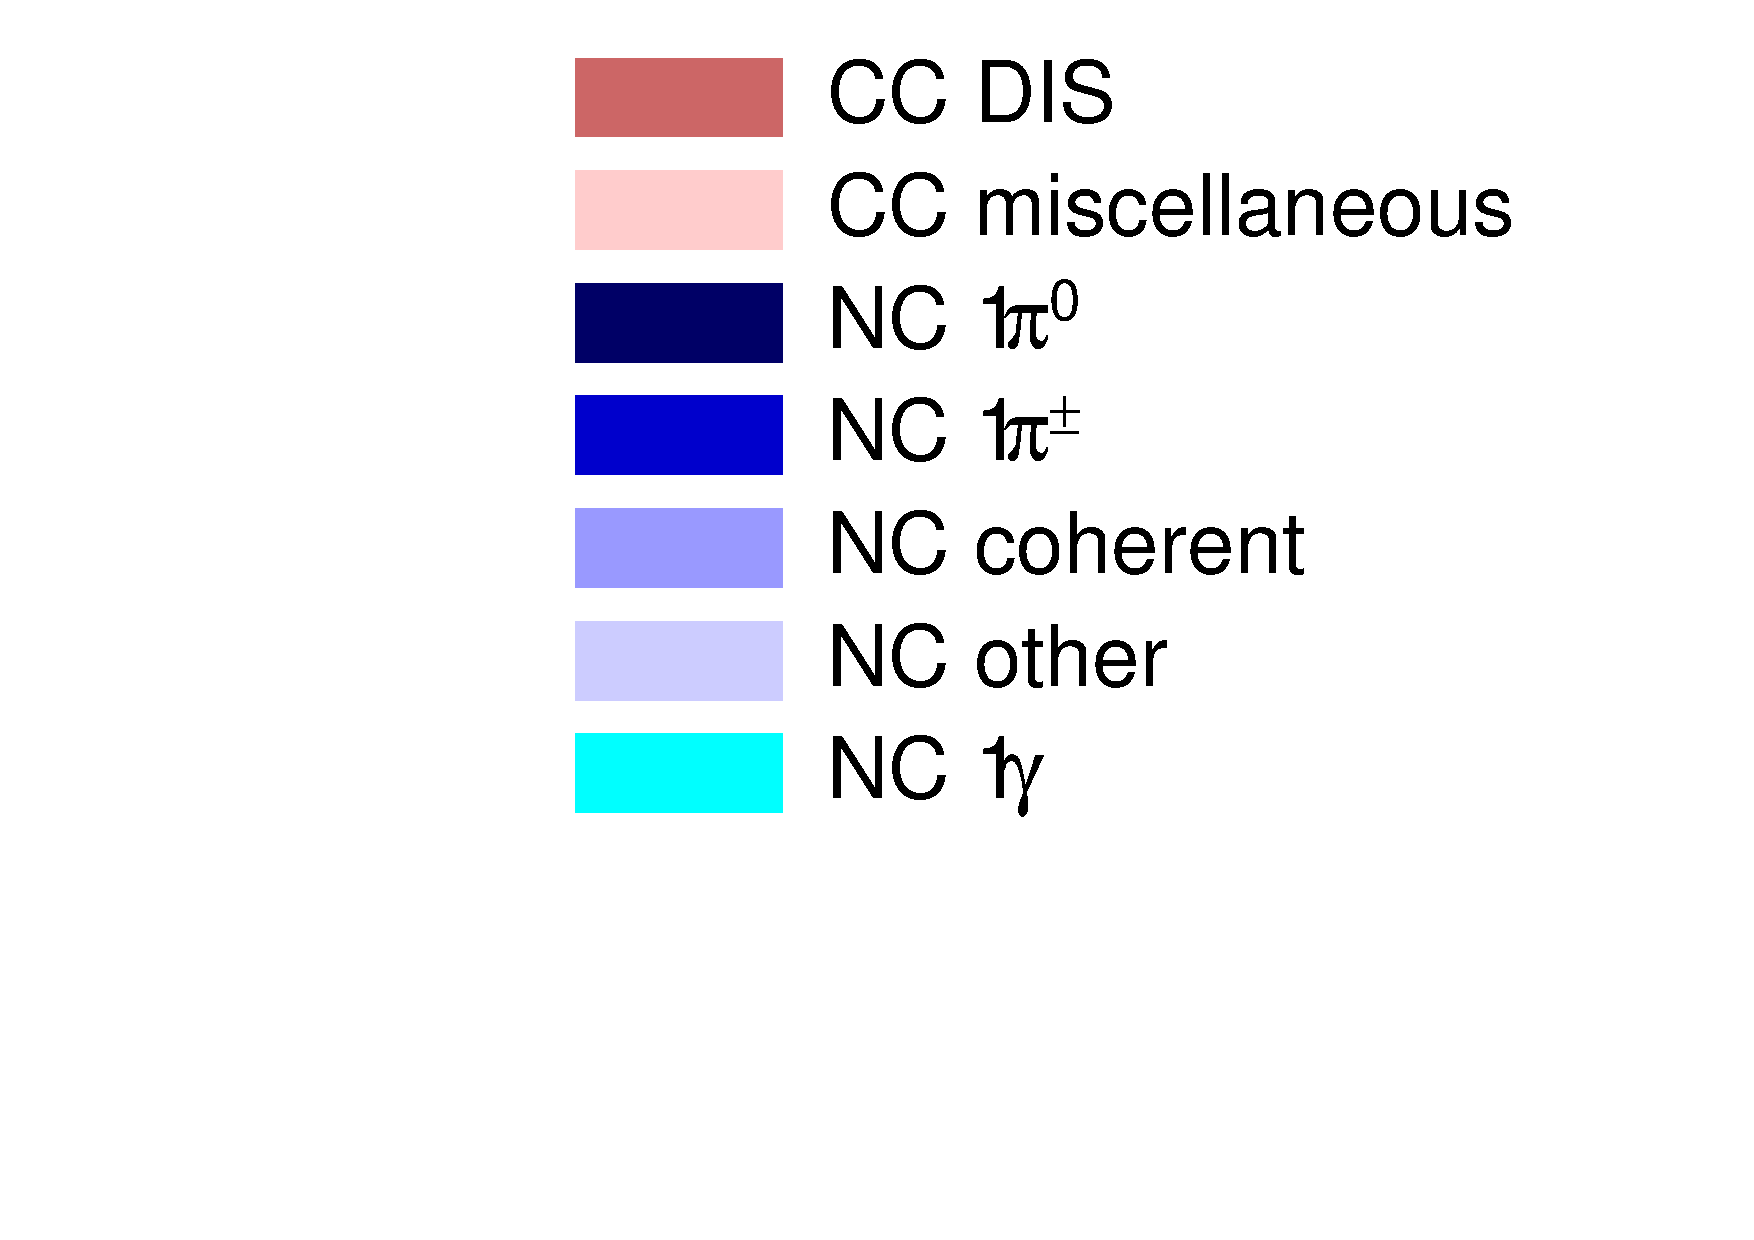
\includegraphics[width=0.7\linewidth]{figs/legend2}
\end{subfigure}
\begin{subfigure}{.32\textwidth}
  \centering
  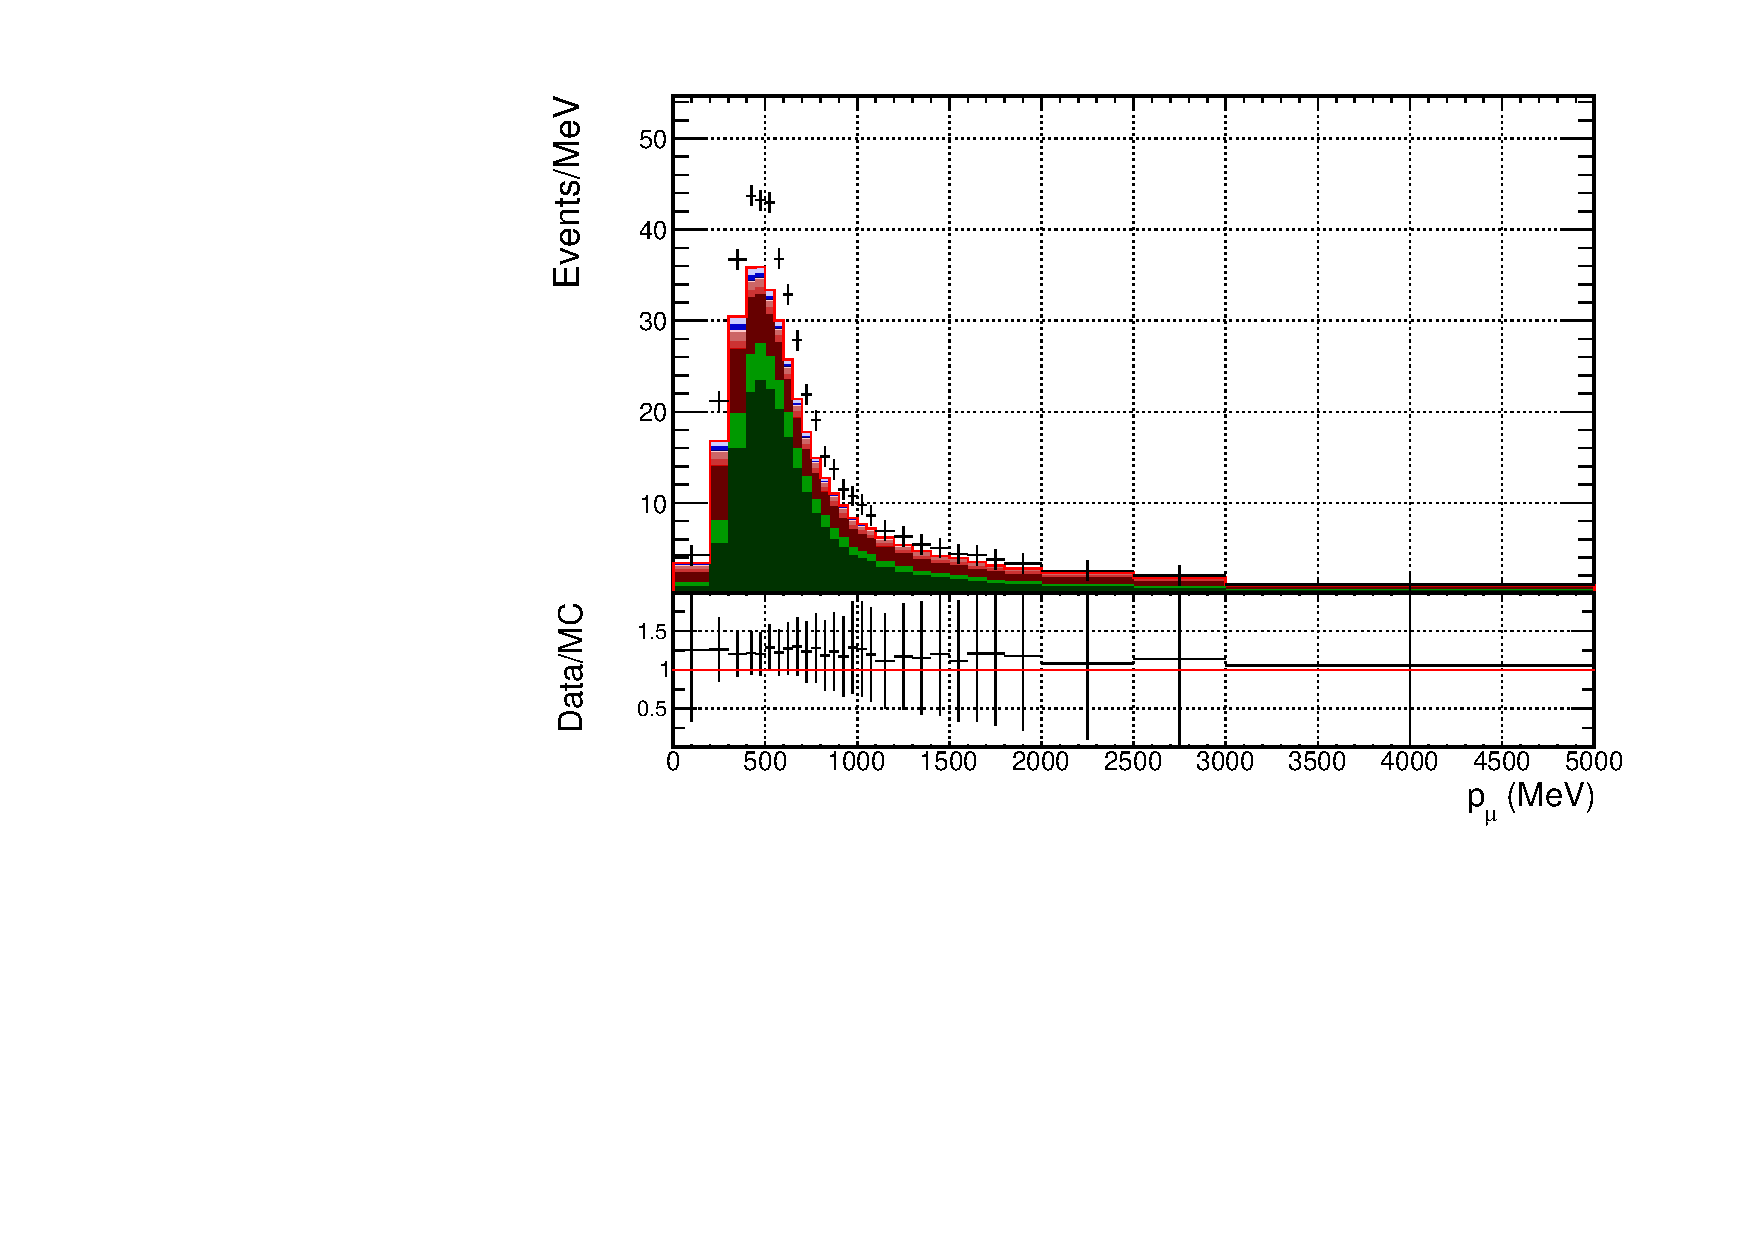
\includegraphics[width=0.95\linewidth]{figs/FGD1_numuCC_0pi_p}
  \caption{FGD1 FHC $\nu_{\mu}$ 0$\pi$}
  \label{fig:pstack_FGD1_numuCC_0pi}
\end{subfigure}
\begin{subfigure}{.32\textwidth}
  \centering
  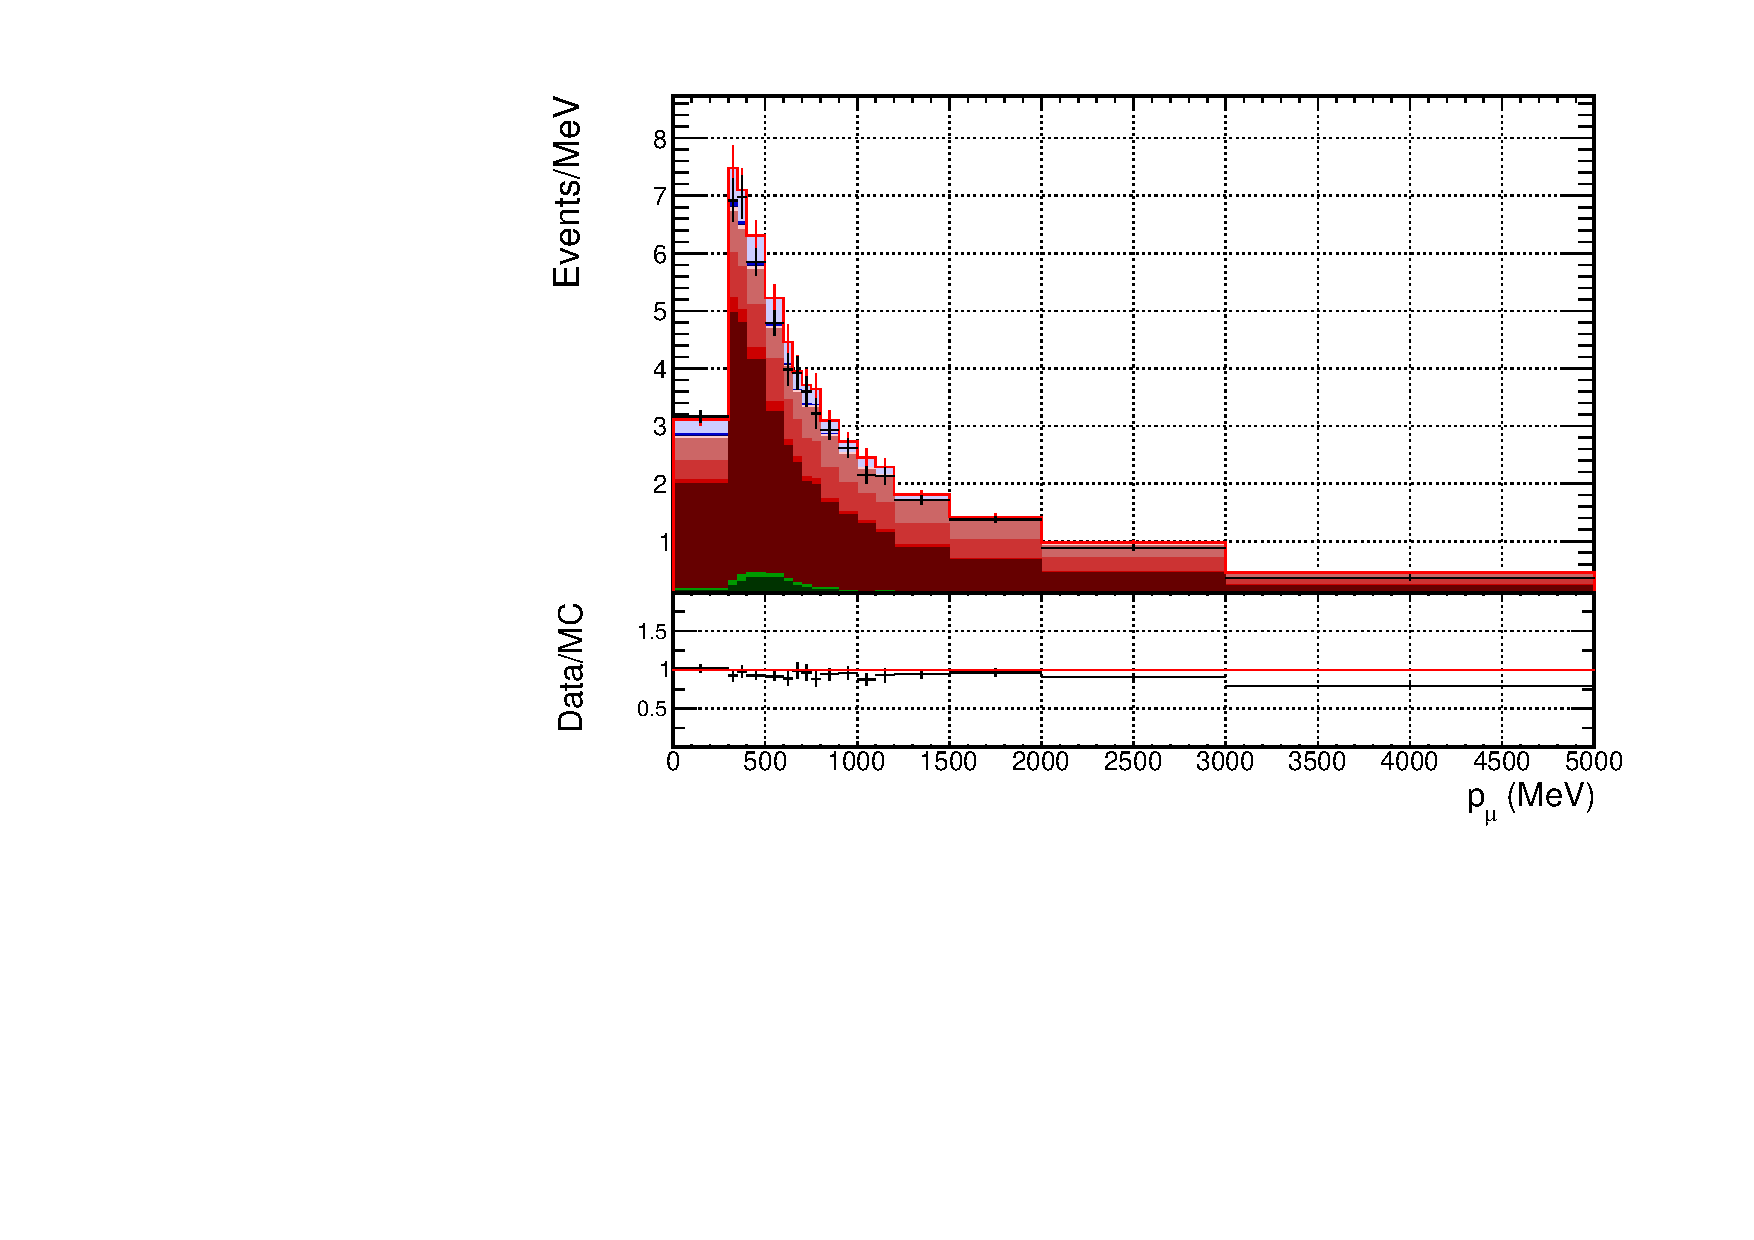
\includegraphics[width=0.95\linewidth]{figs/FGD1_numuCC_1pi_p}
  \caption{FGD1 FHC $\nu_{\mu}$ 1$\pi$}
  \label{fig:pstack_FGD1_numuCC_1pi}
\end{subfigure}
\begin{subfigure}{.32\textwidth}
  \centering
  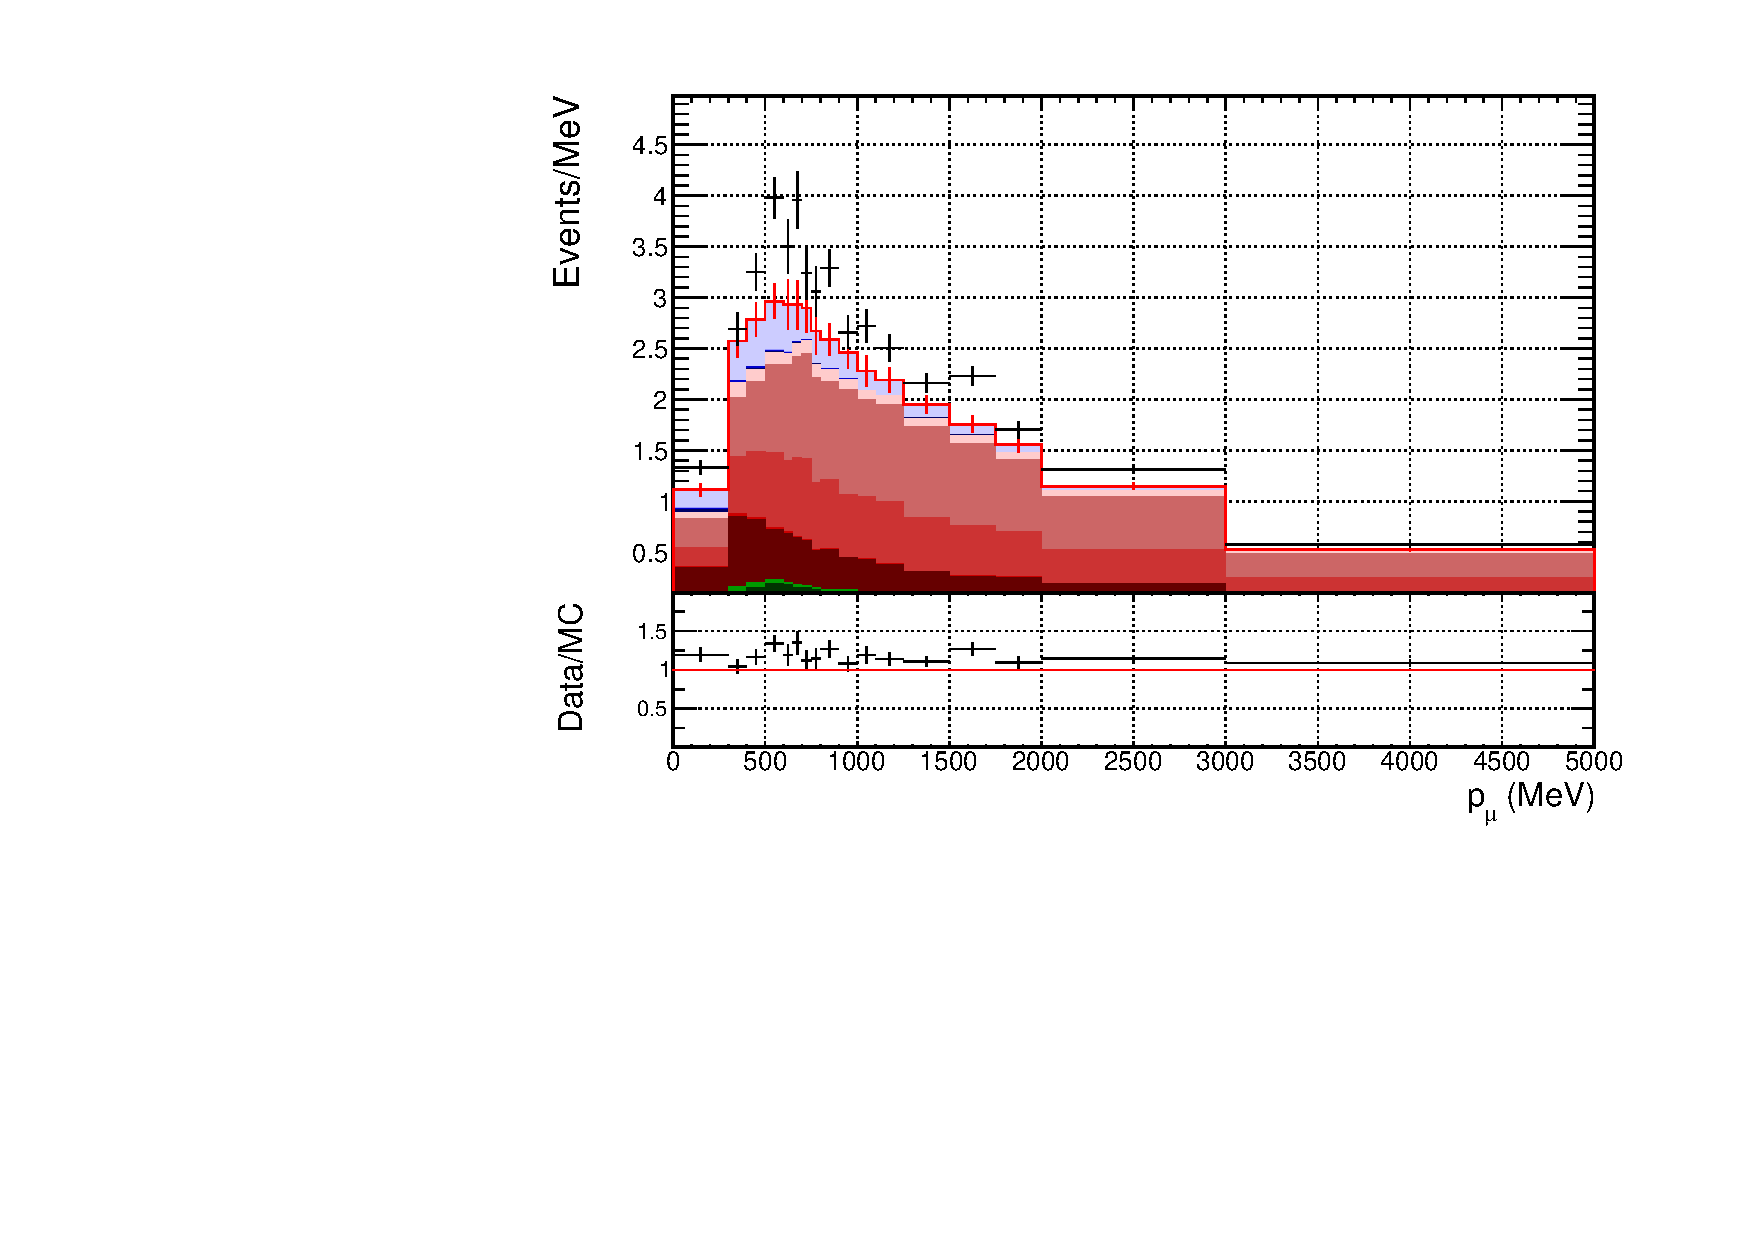
\includegraphics[width=0.95\linewidth]{figs/FGD1_numuCC_other_p}
  \caption{FGD1 FHC $\nu_{\mu}$ Other}
  \label{fig:pstack_FGD1_numuCC_other}
\end{subfigure}
\centering
\begin{subfigure}{.32\textwidth}
  \centering
  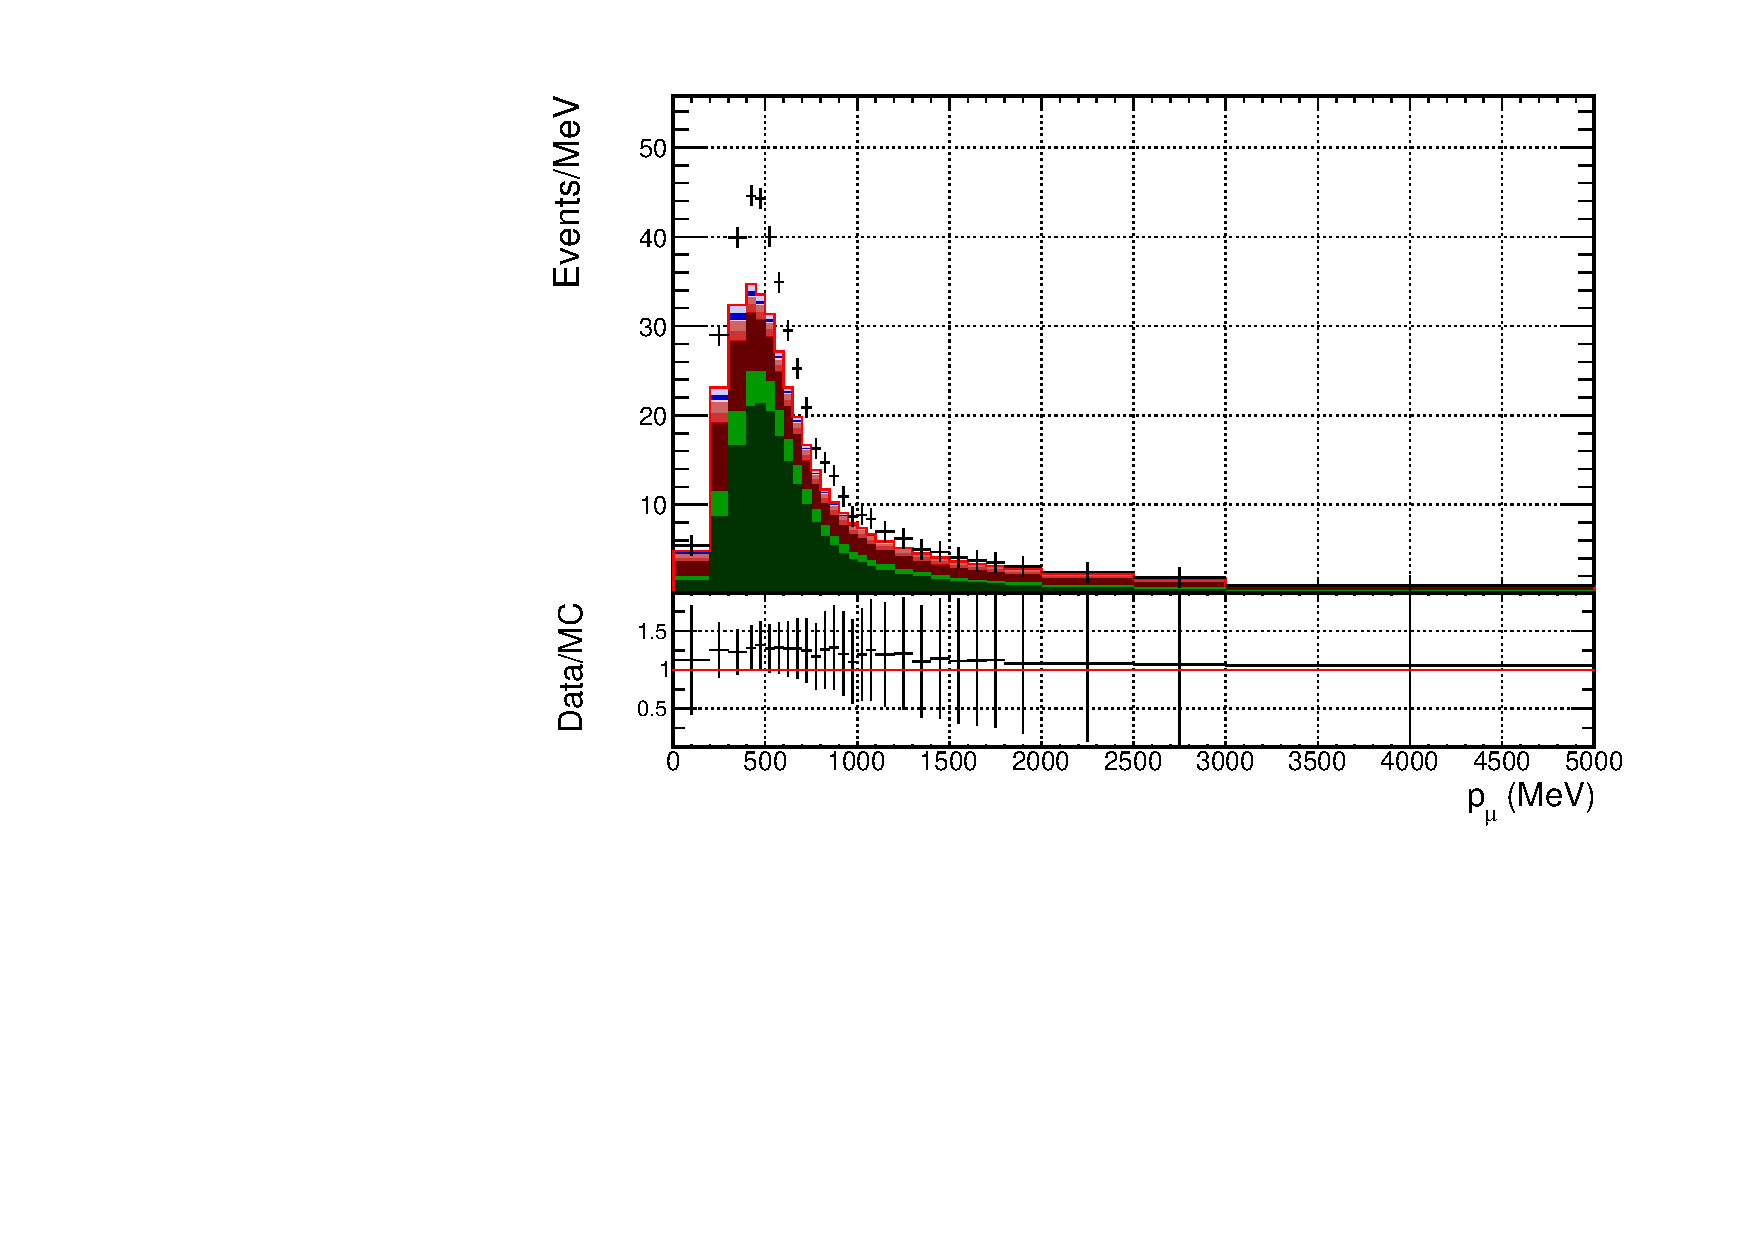
\includegraphics[width=0.95\linewidth]{figs/FGD2_numuCC_0pi_p}
  \caption{FGD2 FHC $\nu_{\mu}$ 0$\pi$}
  \label{fig:pstack_FGD2_numuCC_0pi}
\end{subfigure}
\begin{subfigure}{.32\textwidth}
  \centering
  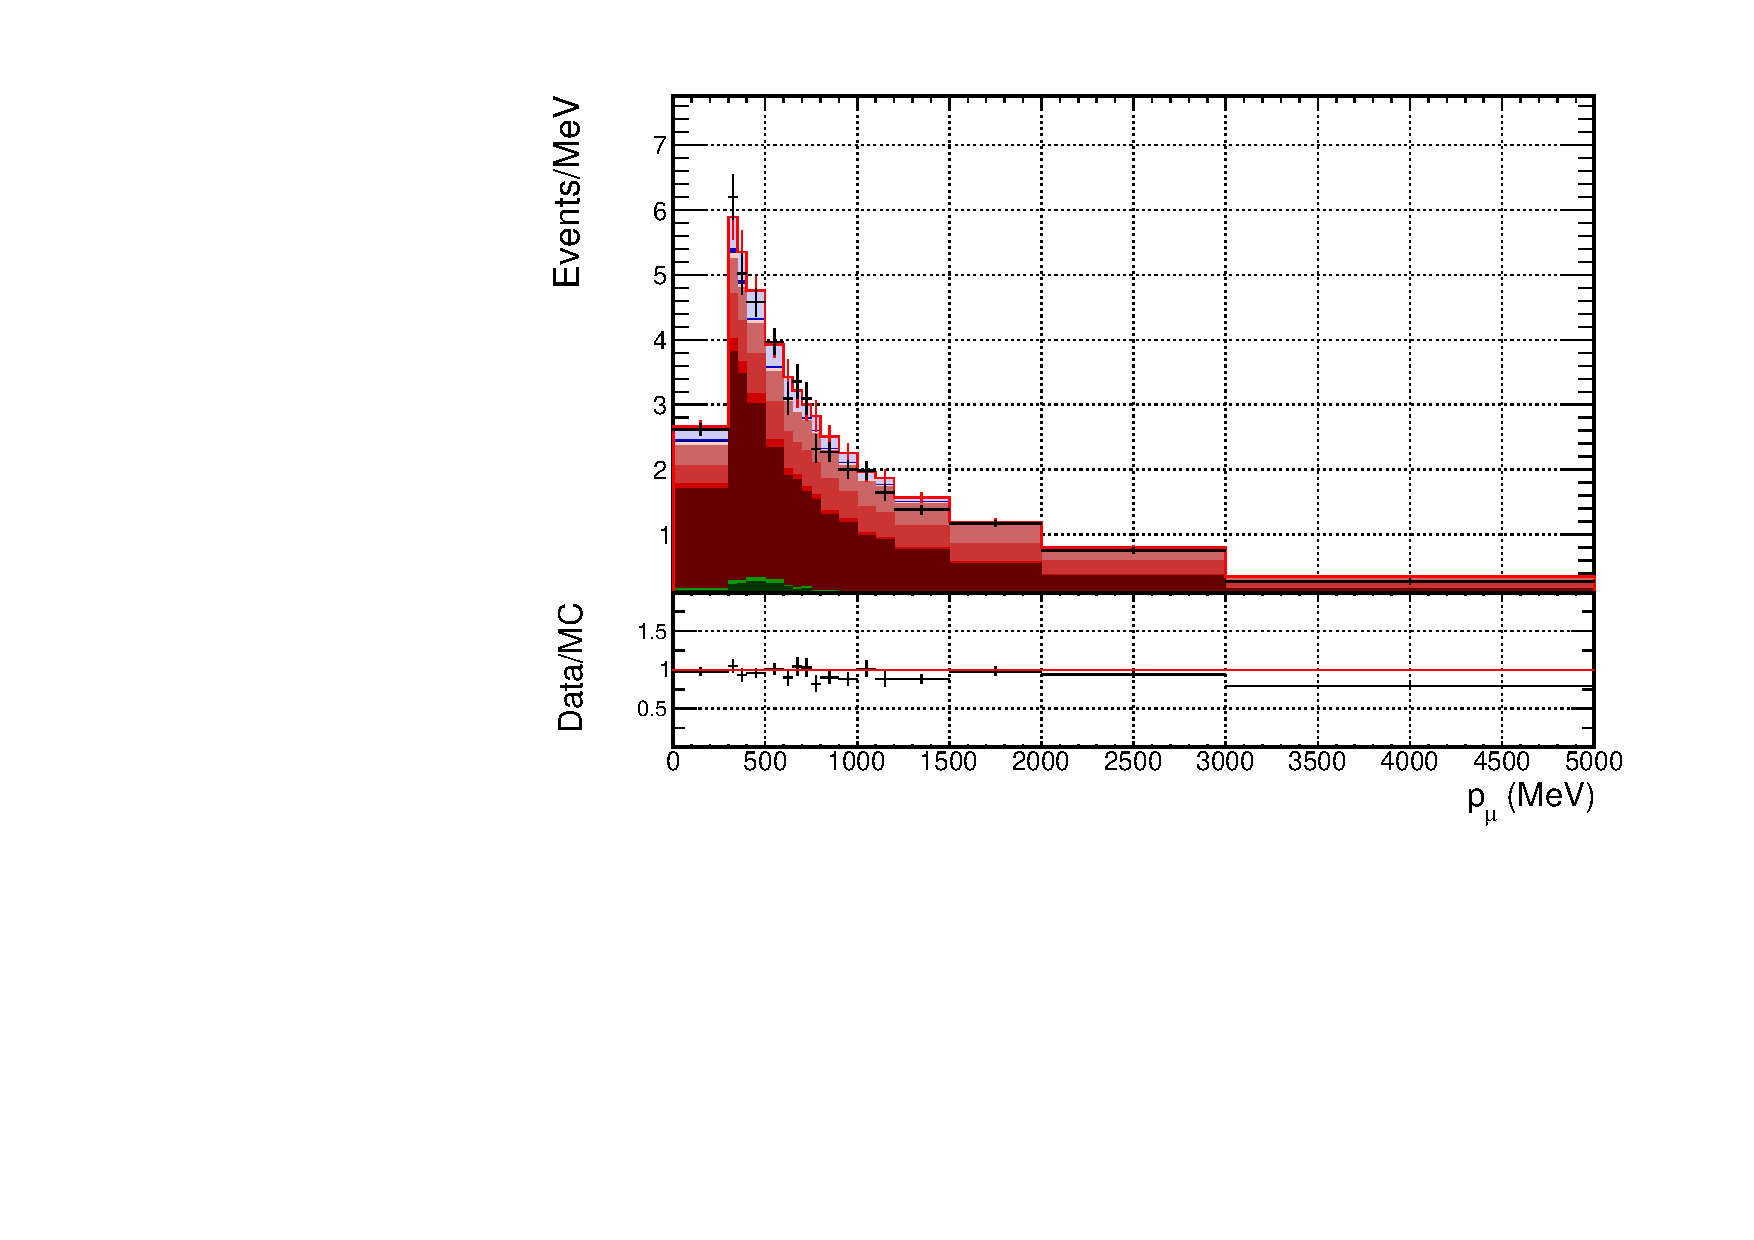
\includegraphics[width=0.95\linewidth]{figs/FGD2_numuCC_1pi_p}
  \caption{FGD2 FHC $\nu_{\mu}$ 1$\pi$}
  \label{fig:pstack_FGD2_numuCC_1pi}
\end{subfigure}
\begin{subfigure}{.32\textwidth}
  \centering
  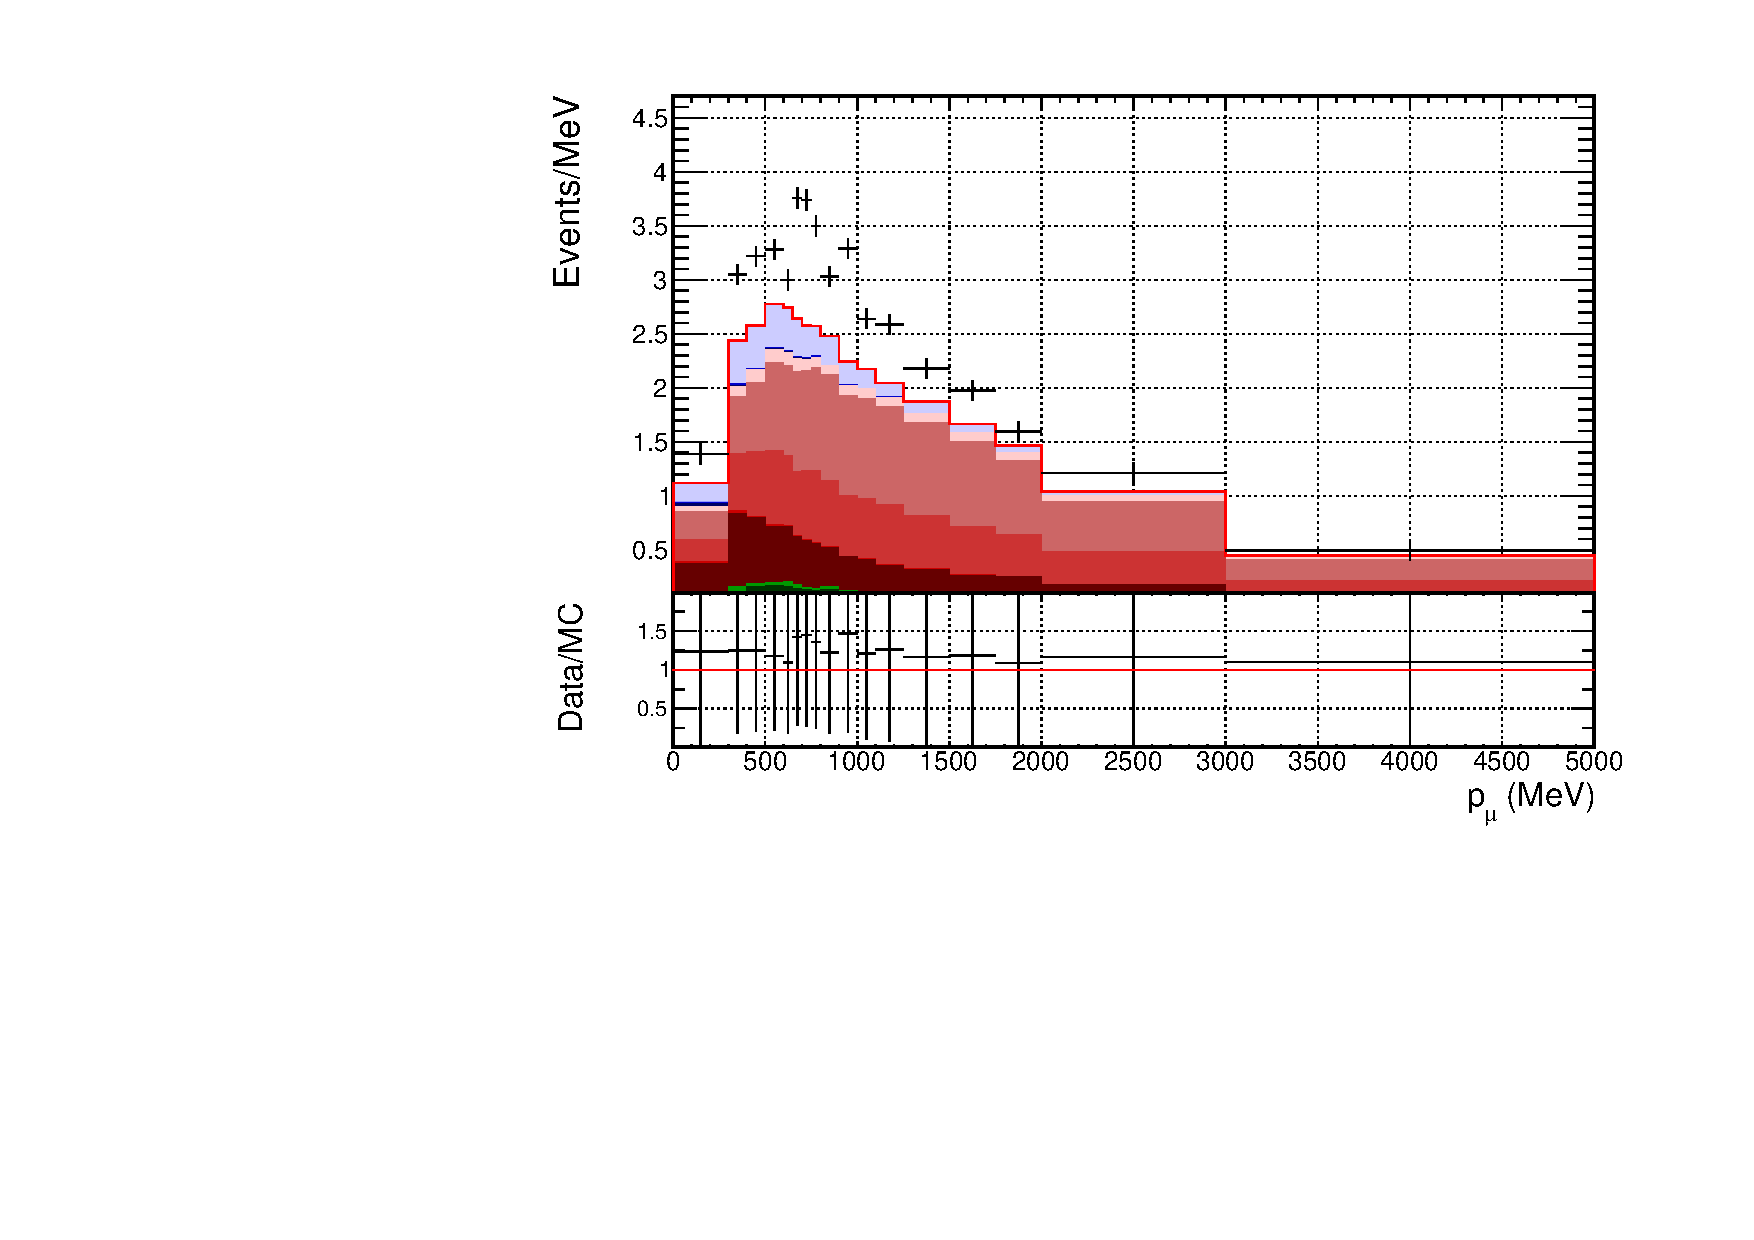
\includegraphics[width=0.95\linewidth]{figs/FGD2_numuCC_other_p}
  \caption{FGD2 $\nu_{\mu}$ Other}
  \label{fig:pstack_FGD2_numuCC_other}
\end{subfigure}
\centering
\begin{subfigure}{.32\textwidth}
  \centering
  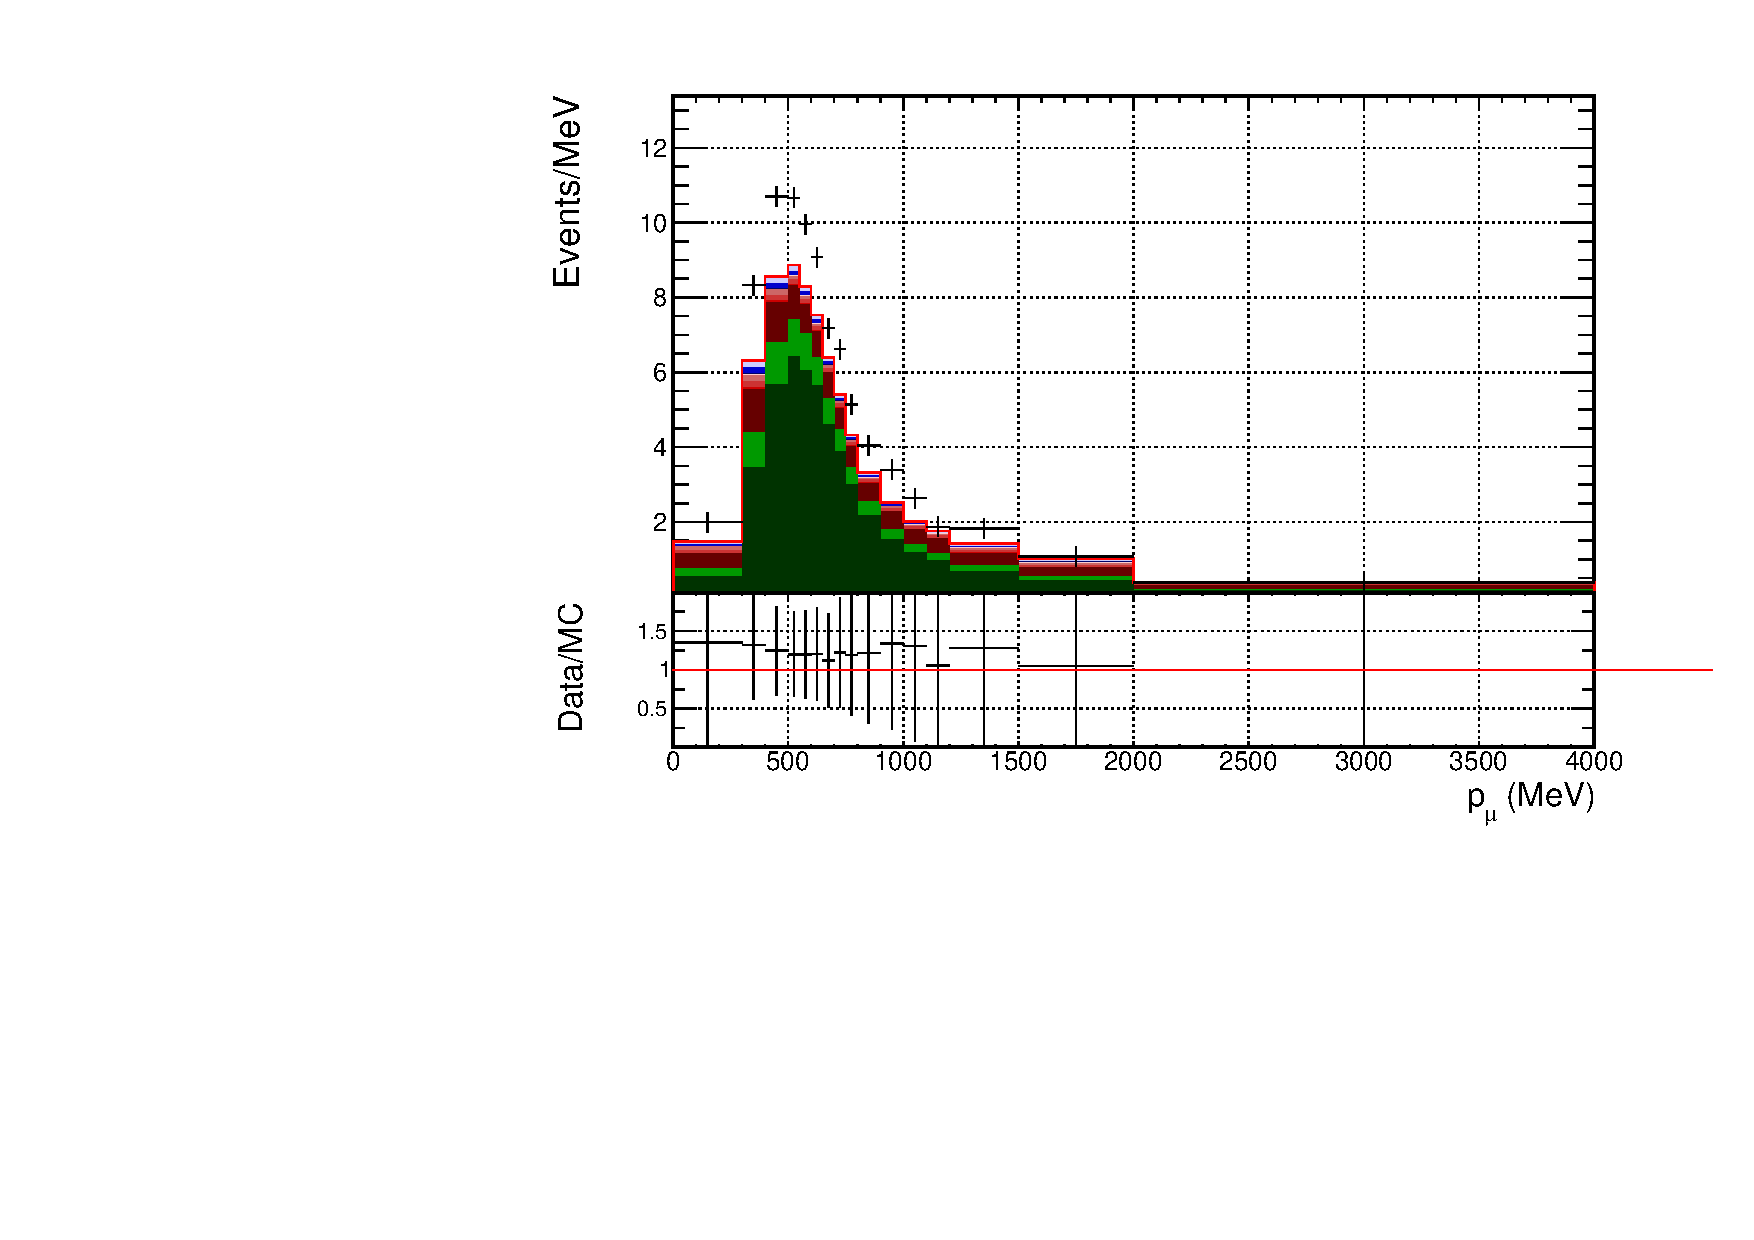
\includegraphics[width=0.95\linewidth]{figs/FGD1_anti-numuCC_0pi_p}
  \caption{FGD1 RHC $\bar{\nu_{\mu}}$ 0$\pi$}
  \label{fig:pstack_FGD1_anti-numuCC_0pi}
\end{subfigure}
\begin{subfigure}{.32\textwidth}
  \centering
  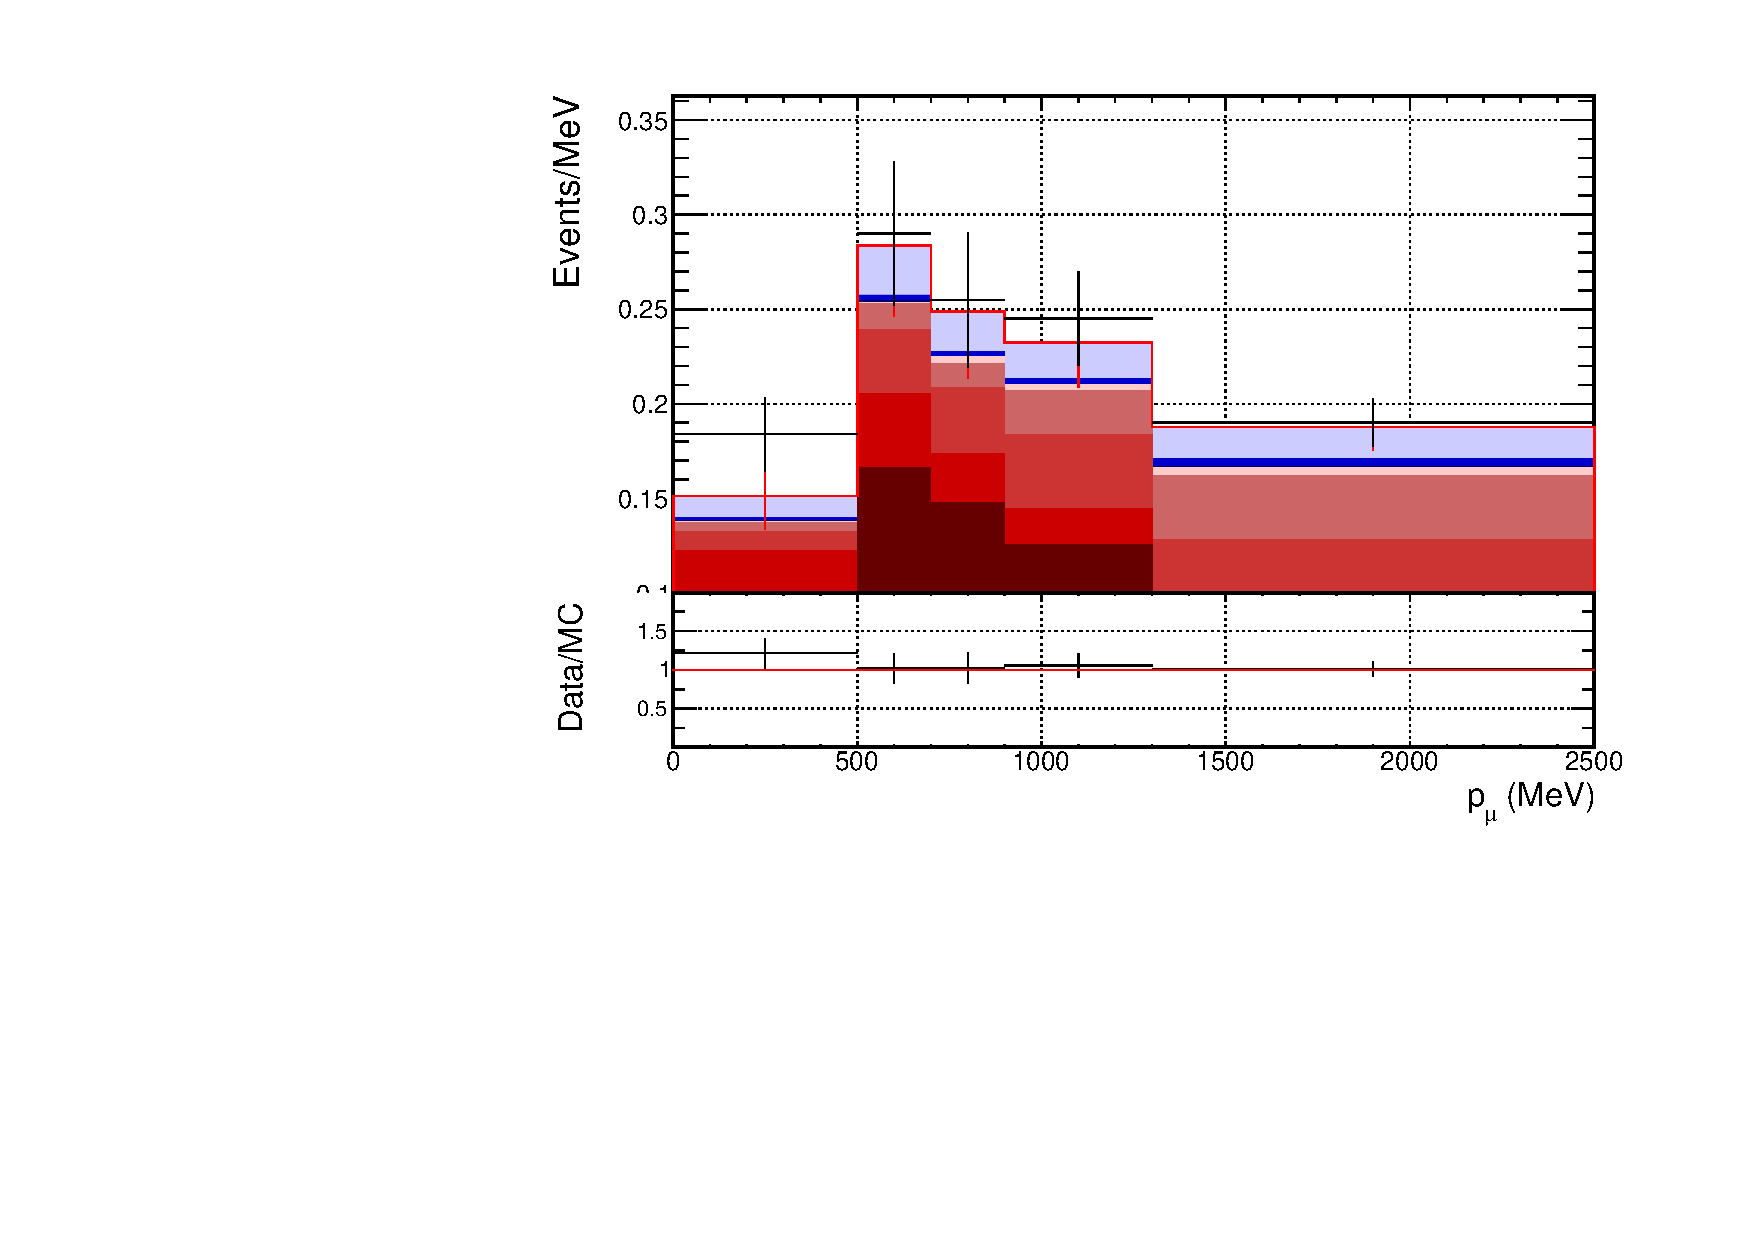
\includegraphics[width=0.95\linewidth]{figs/FGD1_anti-numuCC_1pi_p}
  \caption{FGD1 RHC $\bar{\nu_{\mu}}$ 1$\pi$}
  \label{fig:pstack_pstack_FGD1_anti-numuCC_1pi}
\end{subfigure}
\begin{subfigure}{.32\textwidth}
  \centering
  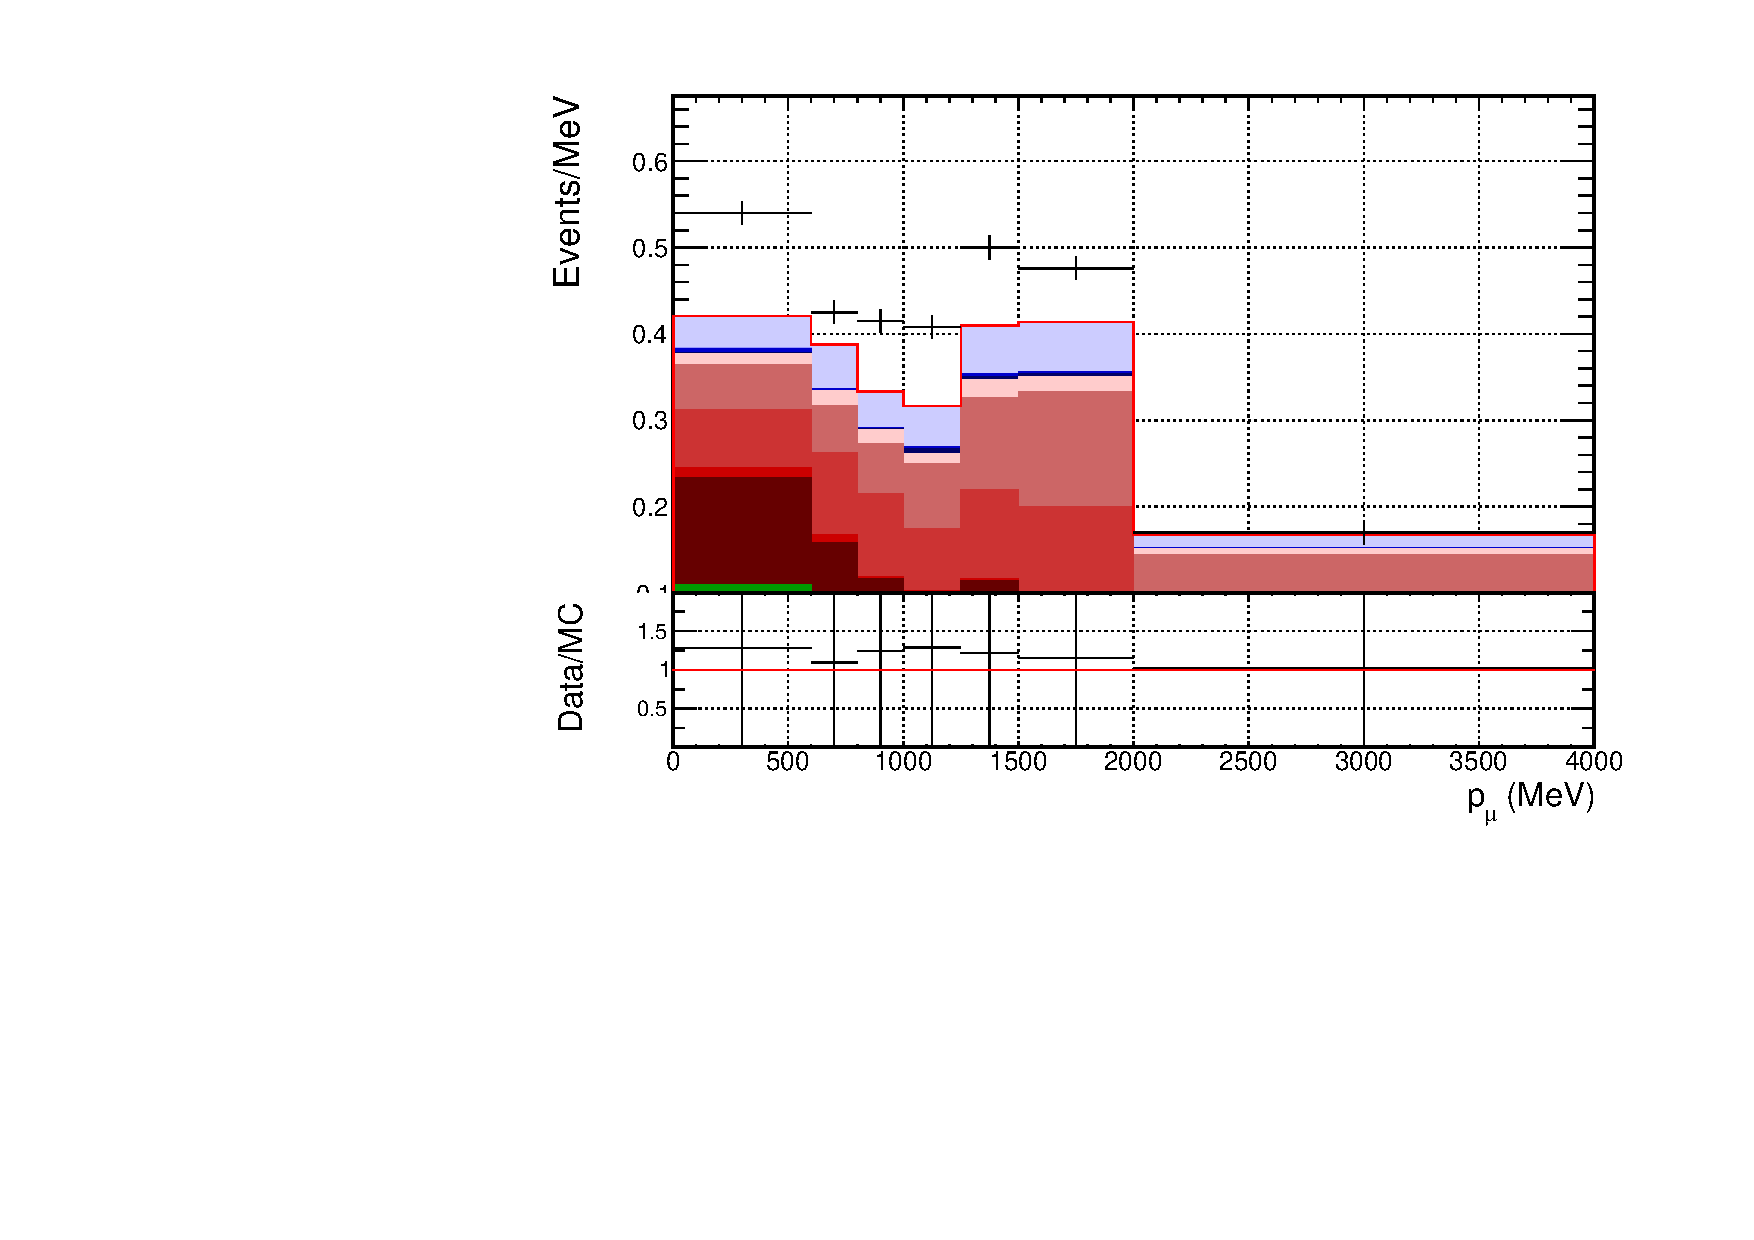
\includegraphics[width=0.95\linewidth]{figs/FGD1_anti-numuCC_other_p}
  \caption{FGD1 RHC $\bar{\nu_{\mu}}$ Other}
  \label{fig:pstack_FGD1_anti-numuCC_other}
\end{subfigure}
\centering
\begin{subfigure}{.32\textwidth}
  \centering
  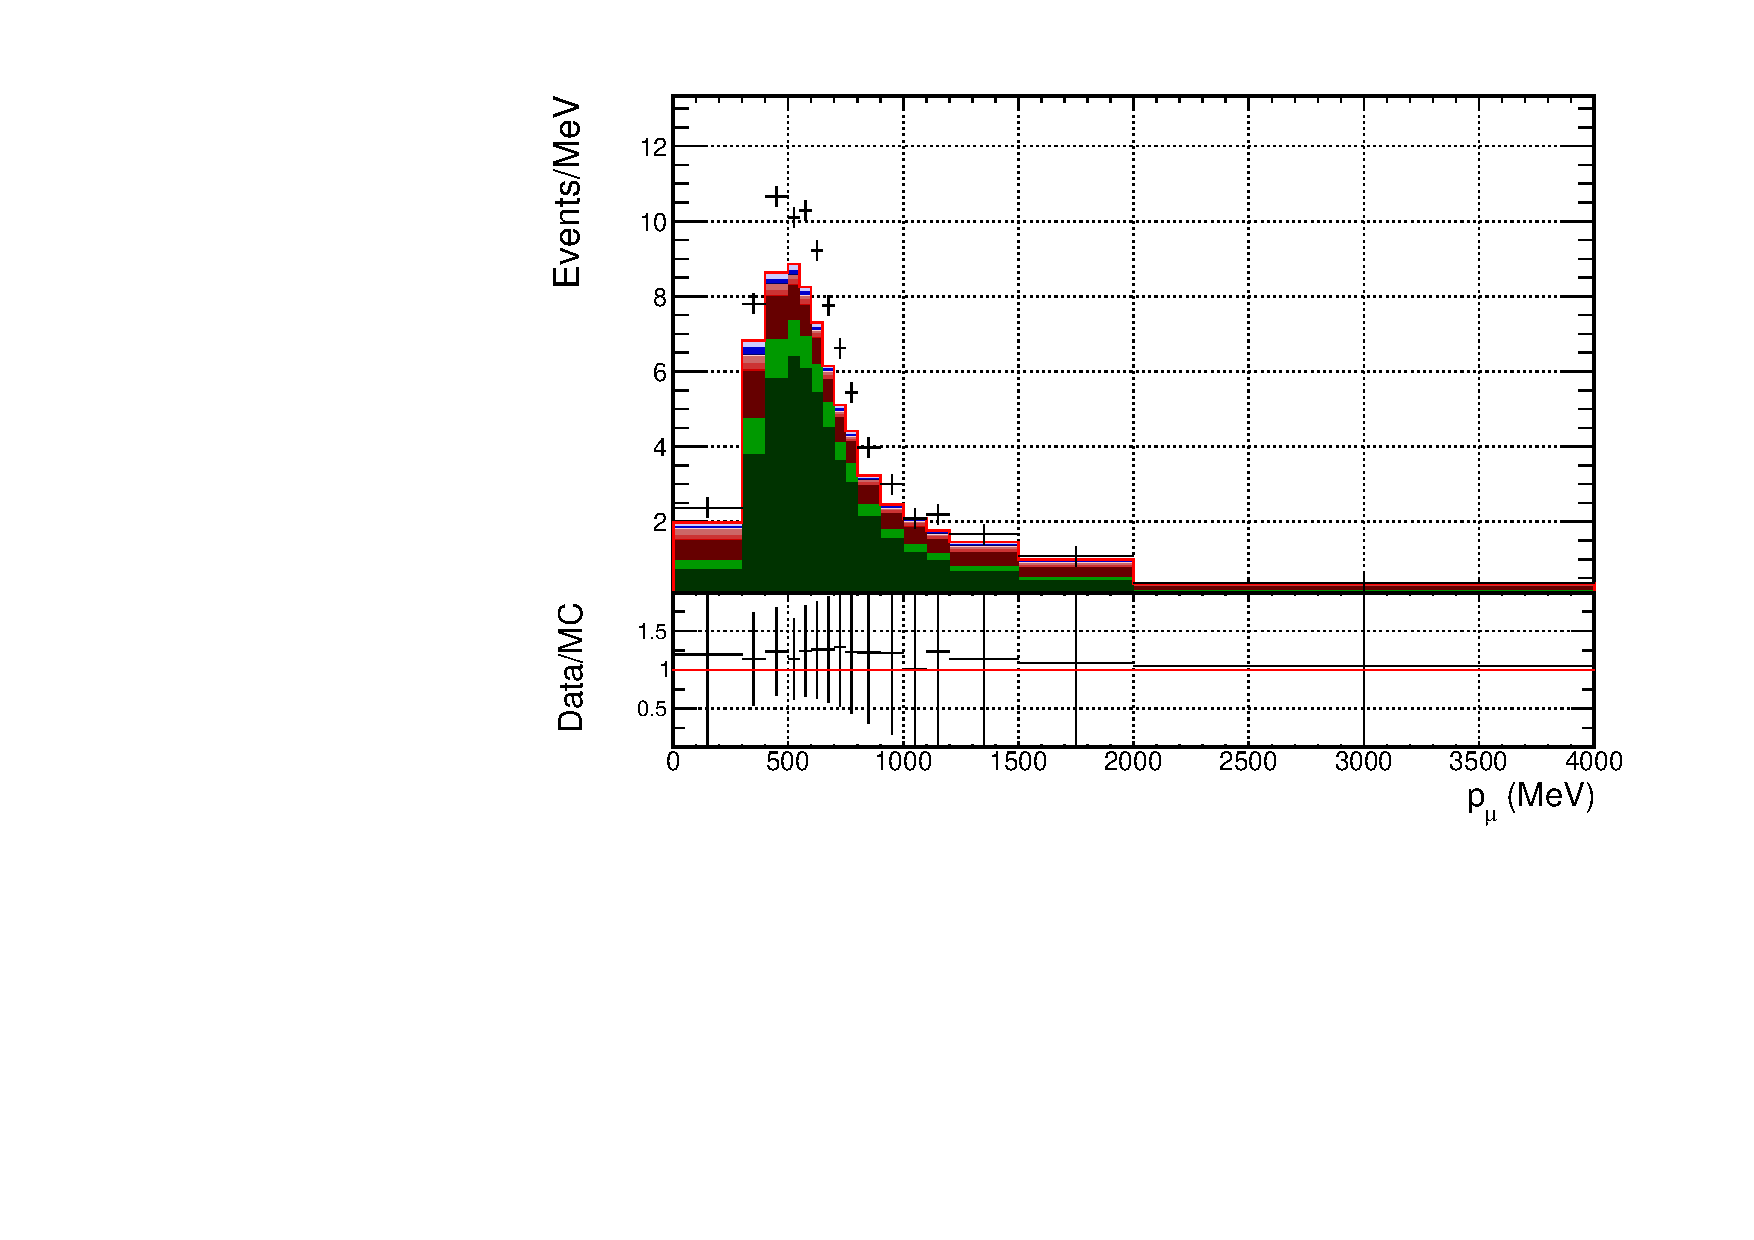
\includegraphics[width=0.95\linewidth]{figs/FGD2_anti-numuCC_0pi_p}
  \caption{FGD2 RHC $\bar{\nu_{\mu}}$ 0$\pi$}
  \label{fig:pstack_FGD2_anti-numuCC_0pi}
\end{subfigure}
\begin{subfigure}{.32\textwidth}
  \centering
  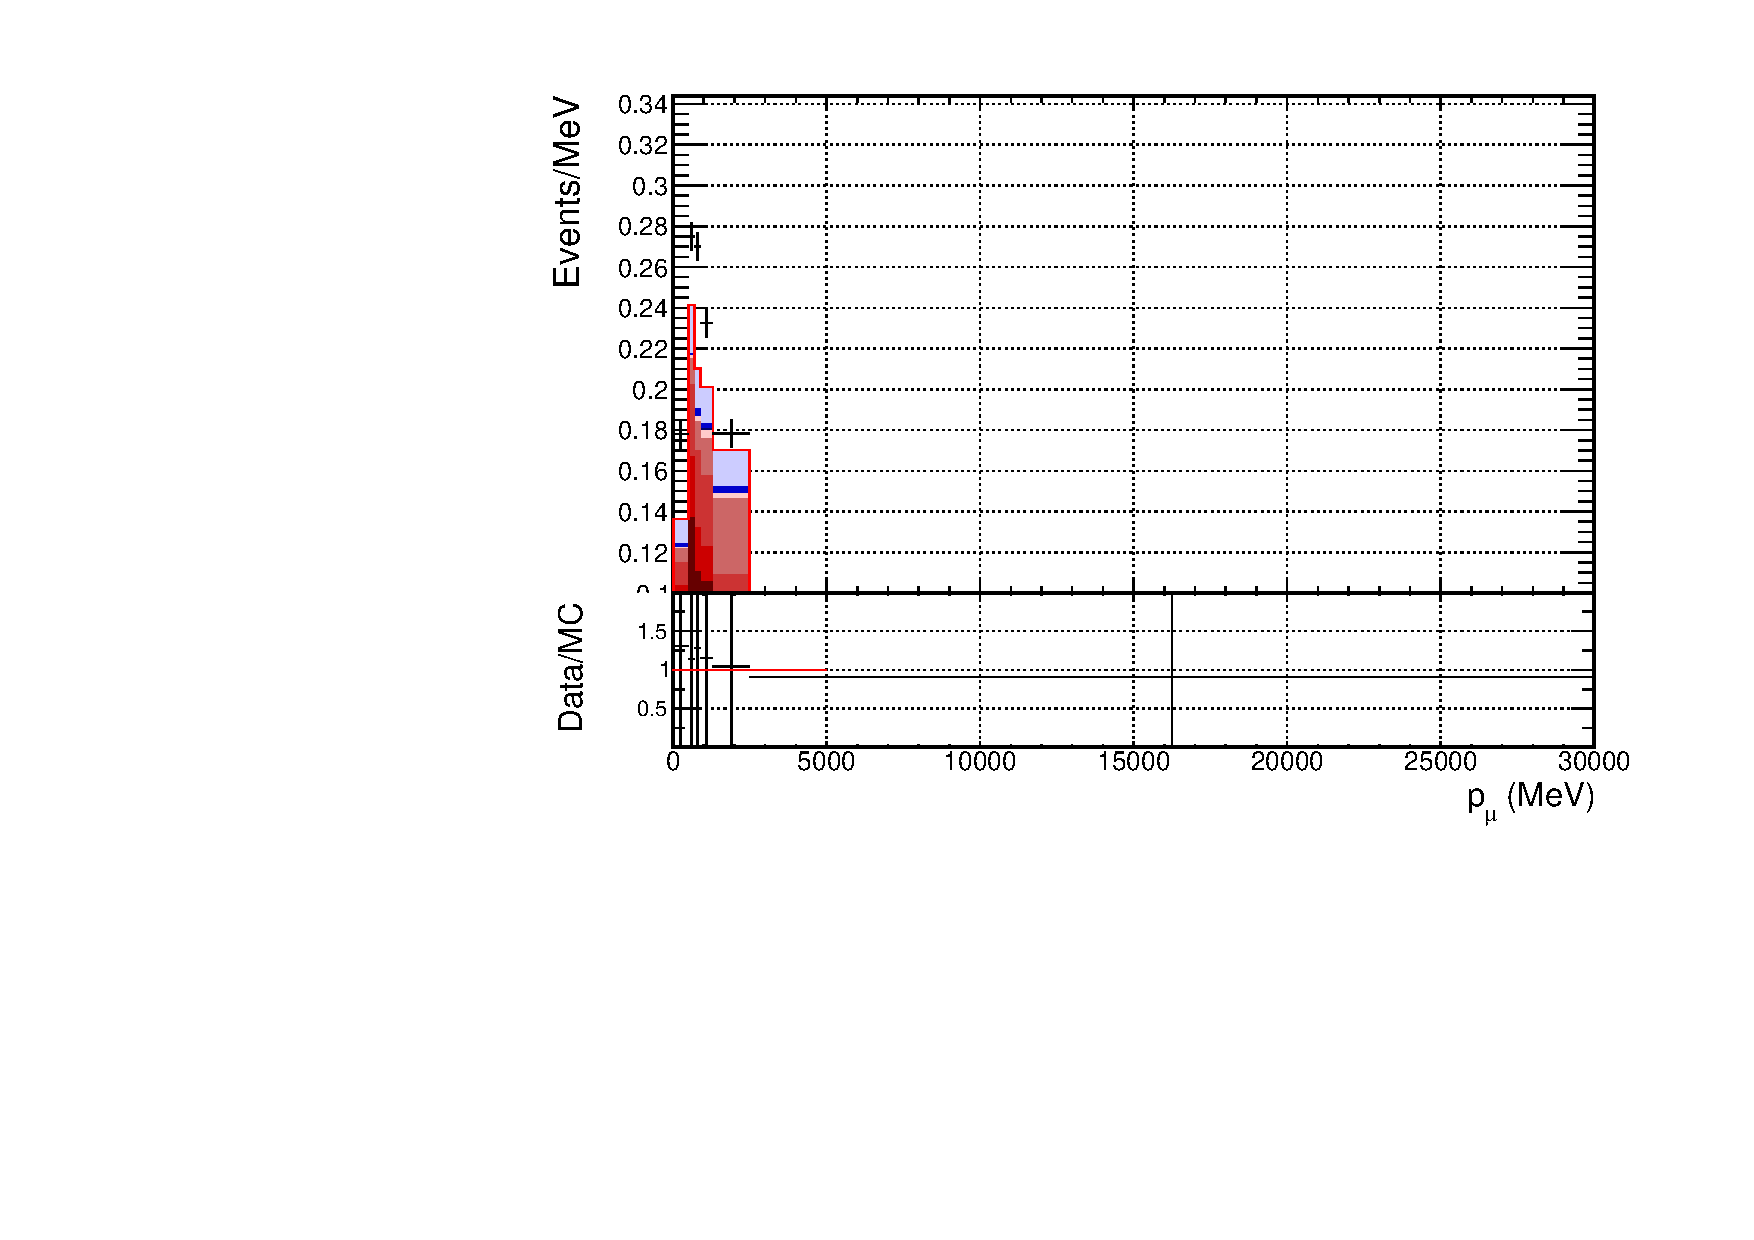
\includegraphics[width=0.95\linewidth]{figs/FGD2_anti-numuCC_1pi_p}
  \caption{FGD2 RHC $\bar{\nu_{\mu}}$ 1$\pi$}
  \label{fig:pstack_pstack_FGD2_anti-numuCC_1pi}
\end{subfigure}
\begin{subfigure}{.32\textwidth}
  \centering
  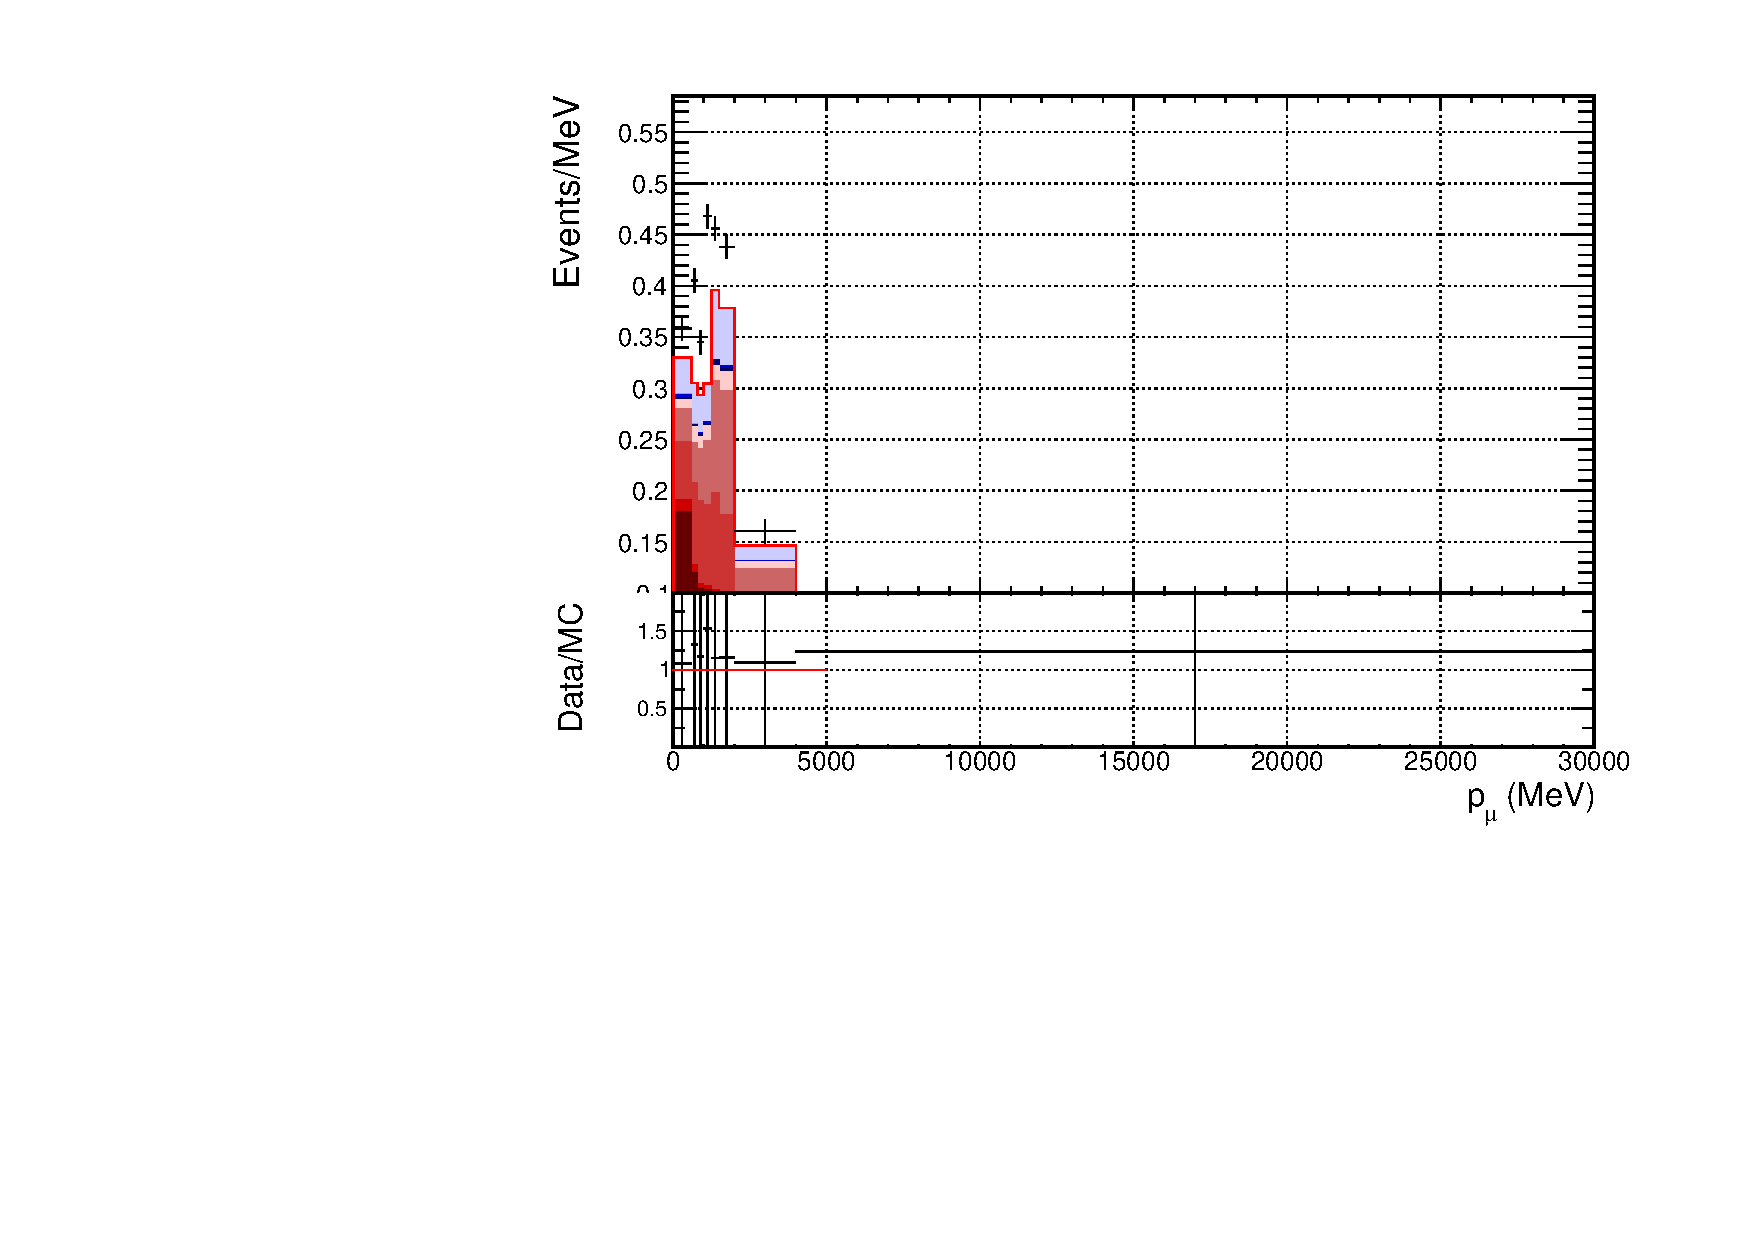
\includegraphics[width=0.95\linewidth]{figs/FGD2_anti-numuCC_other_p}
  \caption{FGD2 RHC $\bar{\nu_{\mu}}$ Other}
  \label{fig:pstack_FGD2_anti-numuCC_other}
\end{subfigure}
\begin{subfigure}{.32\textwidth}
  \centering
  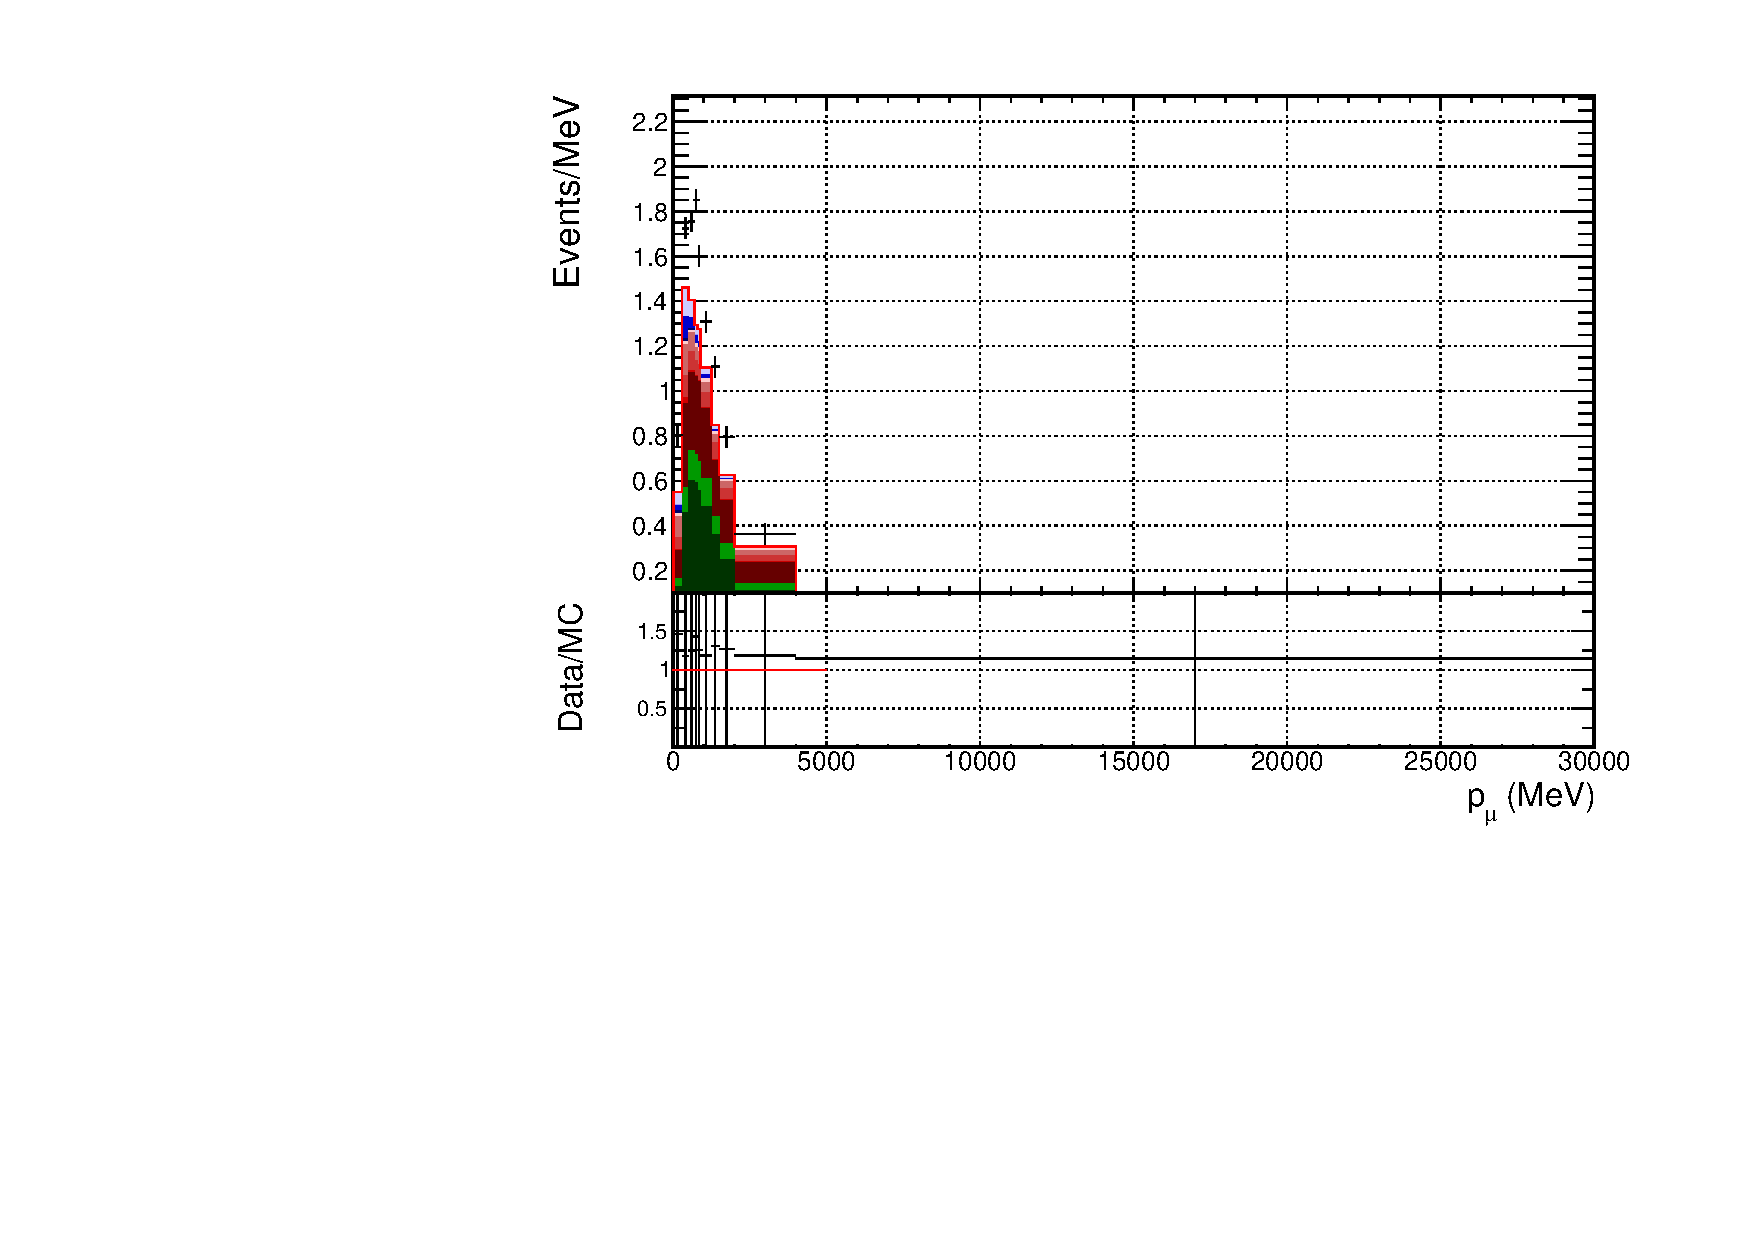
\includegraphics[width=0.95\linewidth]{figs/FGD1_NuMuBkg_CC0pi_in_AntiNu_Mode_p}
  \caption{FGD1 RHC $\nu_{\mu}$ 0$\pi$}
  \label{fig:pstack_FGD1_NuMuBkg_CC0pi_in_AntiNu_Mode}
\end{subfigure}
\begin{subfigure}{.32\textwidth}
  \centering
  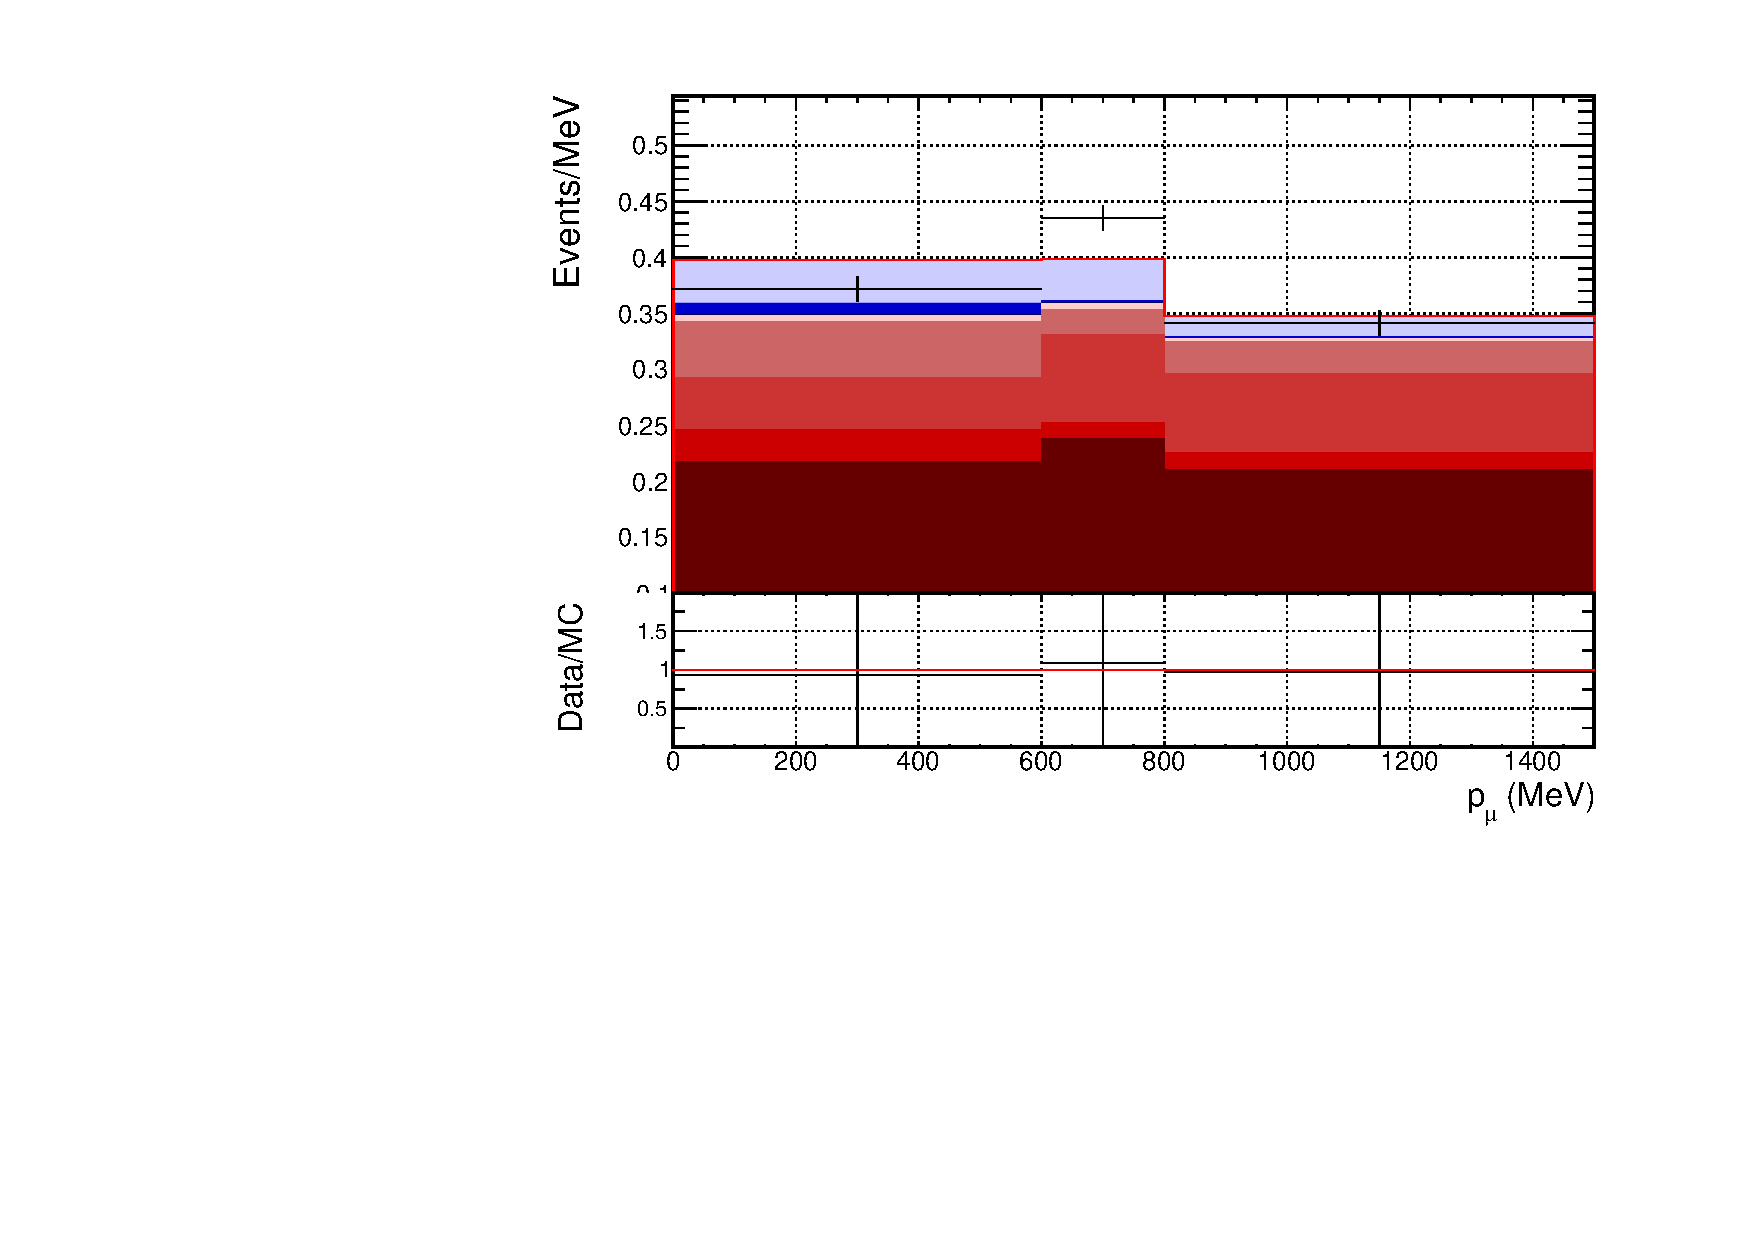
\includegraphics[width=0.95\linewidth]{figs/FGD1_NuMuBkg_CC1pi_in_AntiNu_Mode_p}
  \caption{FGD1 RHC $\nu_{\mu}$ 1$\pi$}
  \label{fig:pstack_FGD1_NuMuBkg_CC1pi_in_AntiNu_Mode}
\end{subfigure}
\begin{subfigure}{.32\textwidth}
  \centering
  \includegraphics[width=0.95\linewidth]{figs/FGD1_NuMuBkg_CCOther_in_AntiNu_Mode_p}
  \caption{FGD1 RHC $\nu_{\mu}$ Other}
  \label{fig:pstack_FGD1_NuMuBkg_CCOther_in_AntiNu_Mode}
\end{subfigure}
\begin{subfigure}{.32\textwidth}
  \centering
  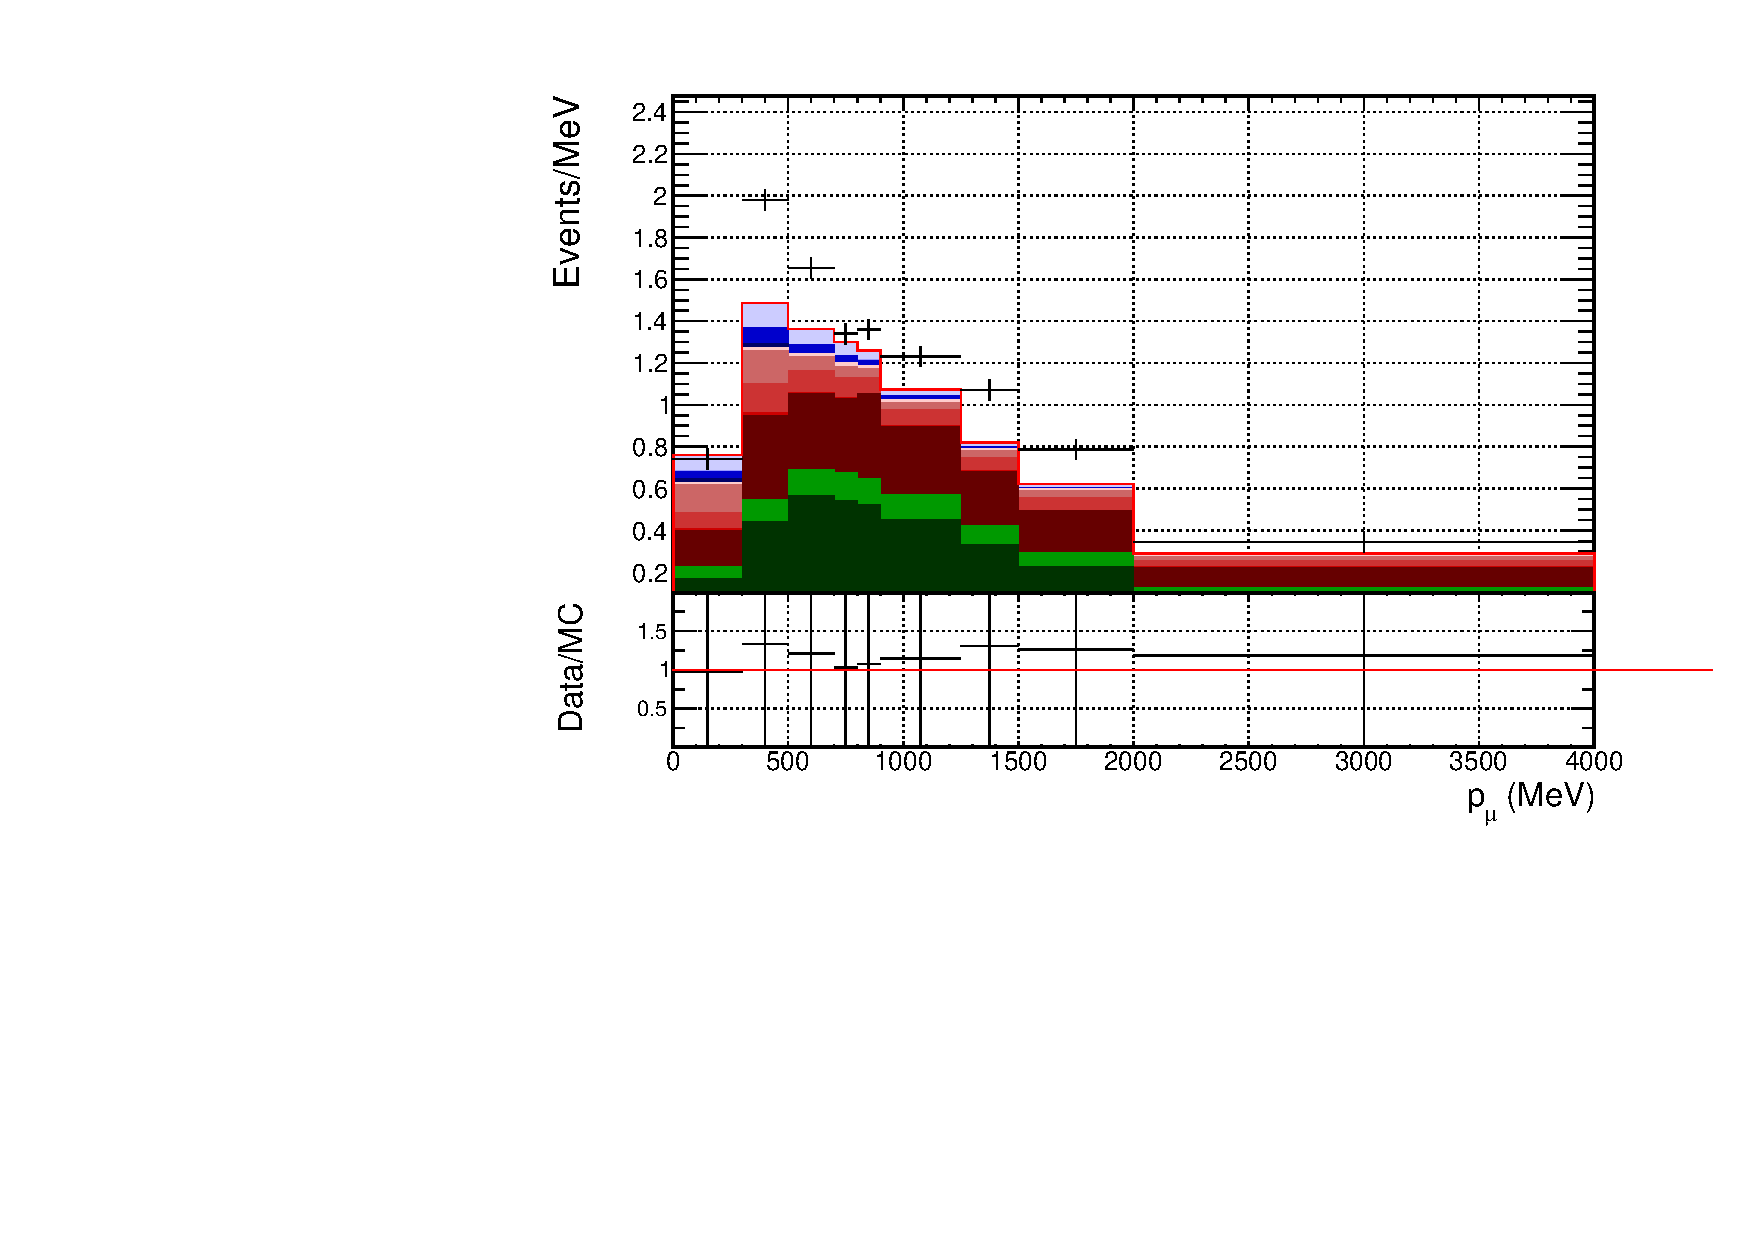
\includegraphics[width=0.95\linewidth]{figs/FGD2_NuMuBkg_CC0pi_in_AntiNu_Mode_p}
  \caption{FGD2 RHC $\nu_{\mu}$ 0$\pi$}
  \label{fig:pstack_FGD2_NuMuBkg_CC0pi_in_AntiNu_Mode}
\end{subfigure}
\begin{subfigure}{.32\textwidth}
  \centering
  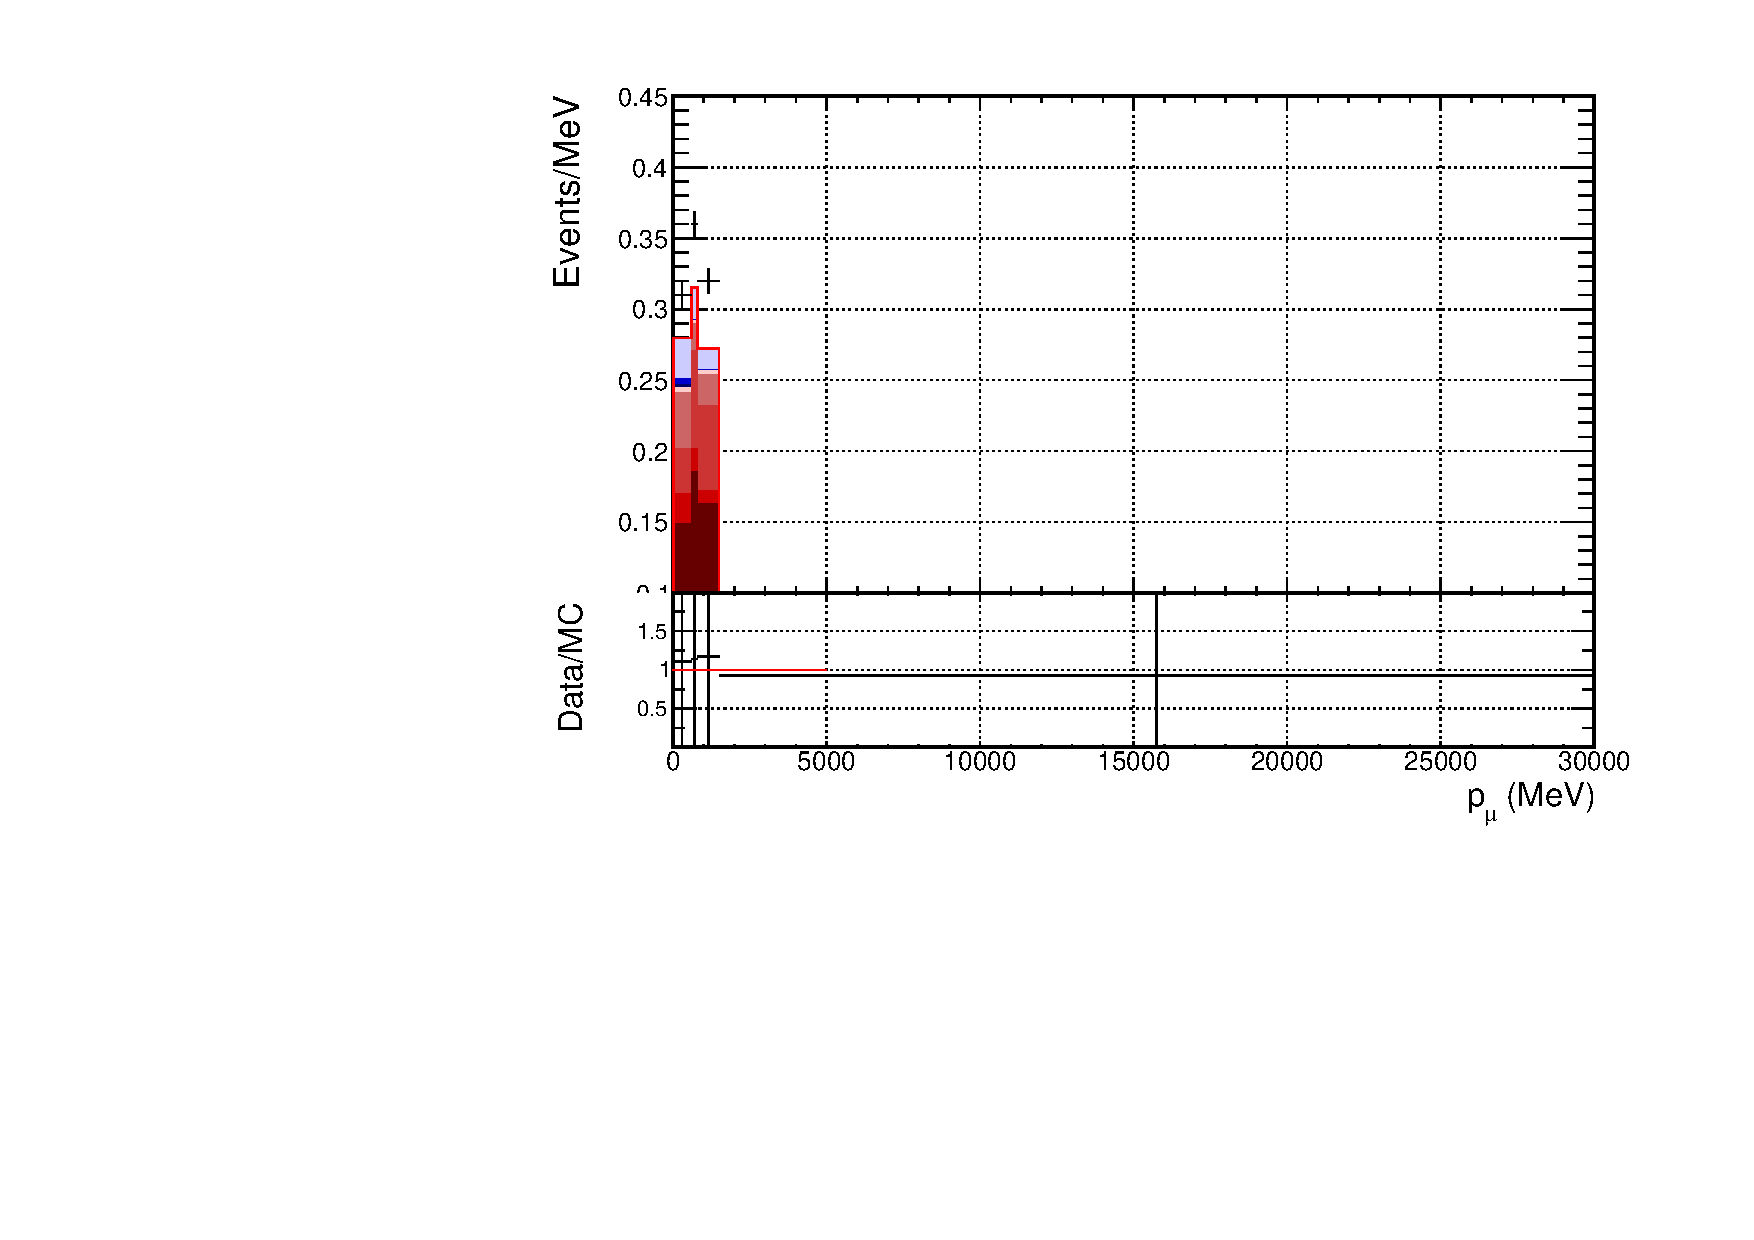
\includegraphics[width=0.95\linewidth]{figs/FGD2_NuMuBkg_CC1pi_in_AntiNu_Mode_p}
  \caption{FGD2 RHC $\nu_{\mu}$ 1$\pi$}
  \label{fig:pstack_FGD2_NuMuBkg_CC1pi_in_AntiNu_Mode}
\end{subfigure}
\begin{subfigure}{.32\textwidth}
  \centering
  \includegraphics[width=0.95\linewidth]{figs/FGD2_NuMuBkg_CCOther_in_AntiNu_Mode_p}
  \caption{FGD2 RHC $\nu_{\mu}$ Other}
  \label{fig:pstack_FGD2_NuMuBkg_CCOther_in_AntiNu_Mode}
\end{subfigure}
\caption{p$_{\mu}$ projections of data and nominal MC broken down by interaction mode.}
\label{fig:pstack}
\end{figure}

The projections onto the cos $\theta_{\mu}$ axis are shown in Figure \ref{fig:tstack}, along with the data and interaction mode breakdown.

The CC 0$\pi$ and CC Other samples again show oscillatory behaviour in the ratio of data to MC. At high angle, the ratio increases and decreases, but always remains $>1$. For the CC 1$\pi$ samples,  the ratio is again more flat, but at high angle oscillates between the MC over and underestimating the data. This is again consistent across the FGDs.

\begin{figure}
\centering
\begin{subfigure}{.35\textwidth}
  \centering
  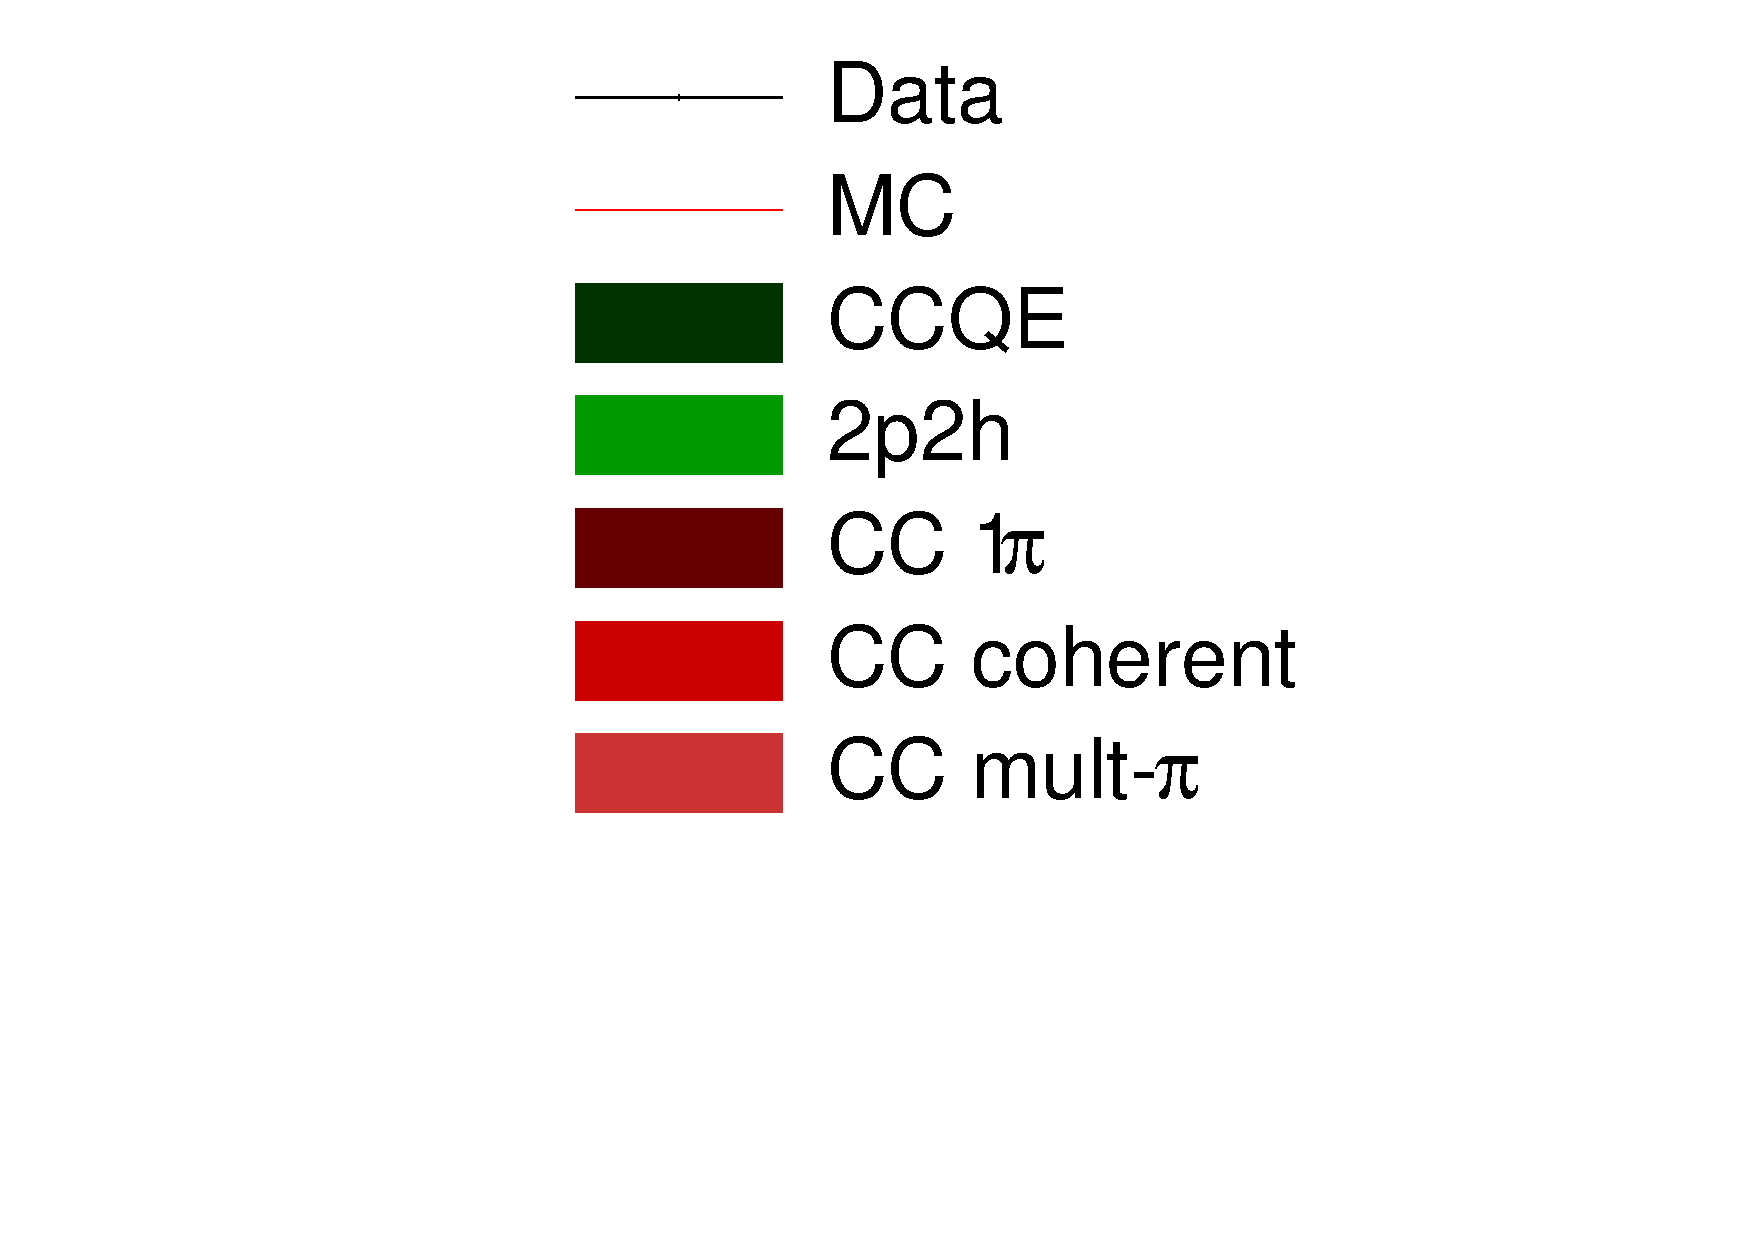
\includegraphics[width=0.7\linewidth]{figs/legend}
\end{subfigure}
\begin{subfigure}{.35\textwidth}
  \centering
  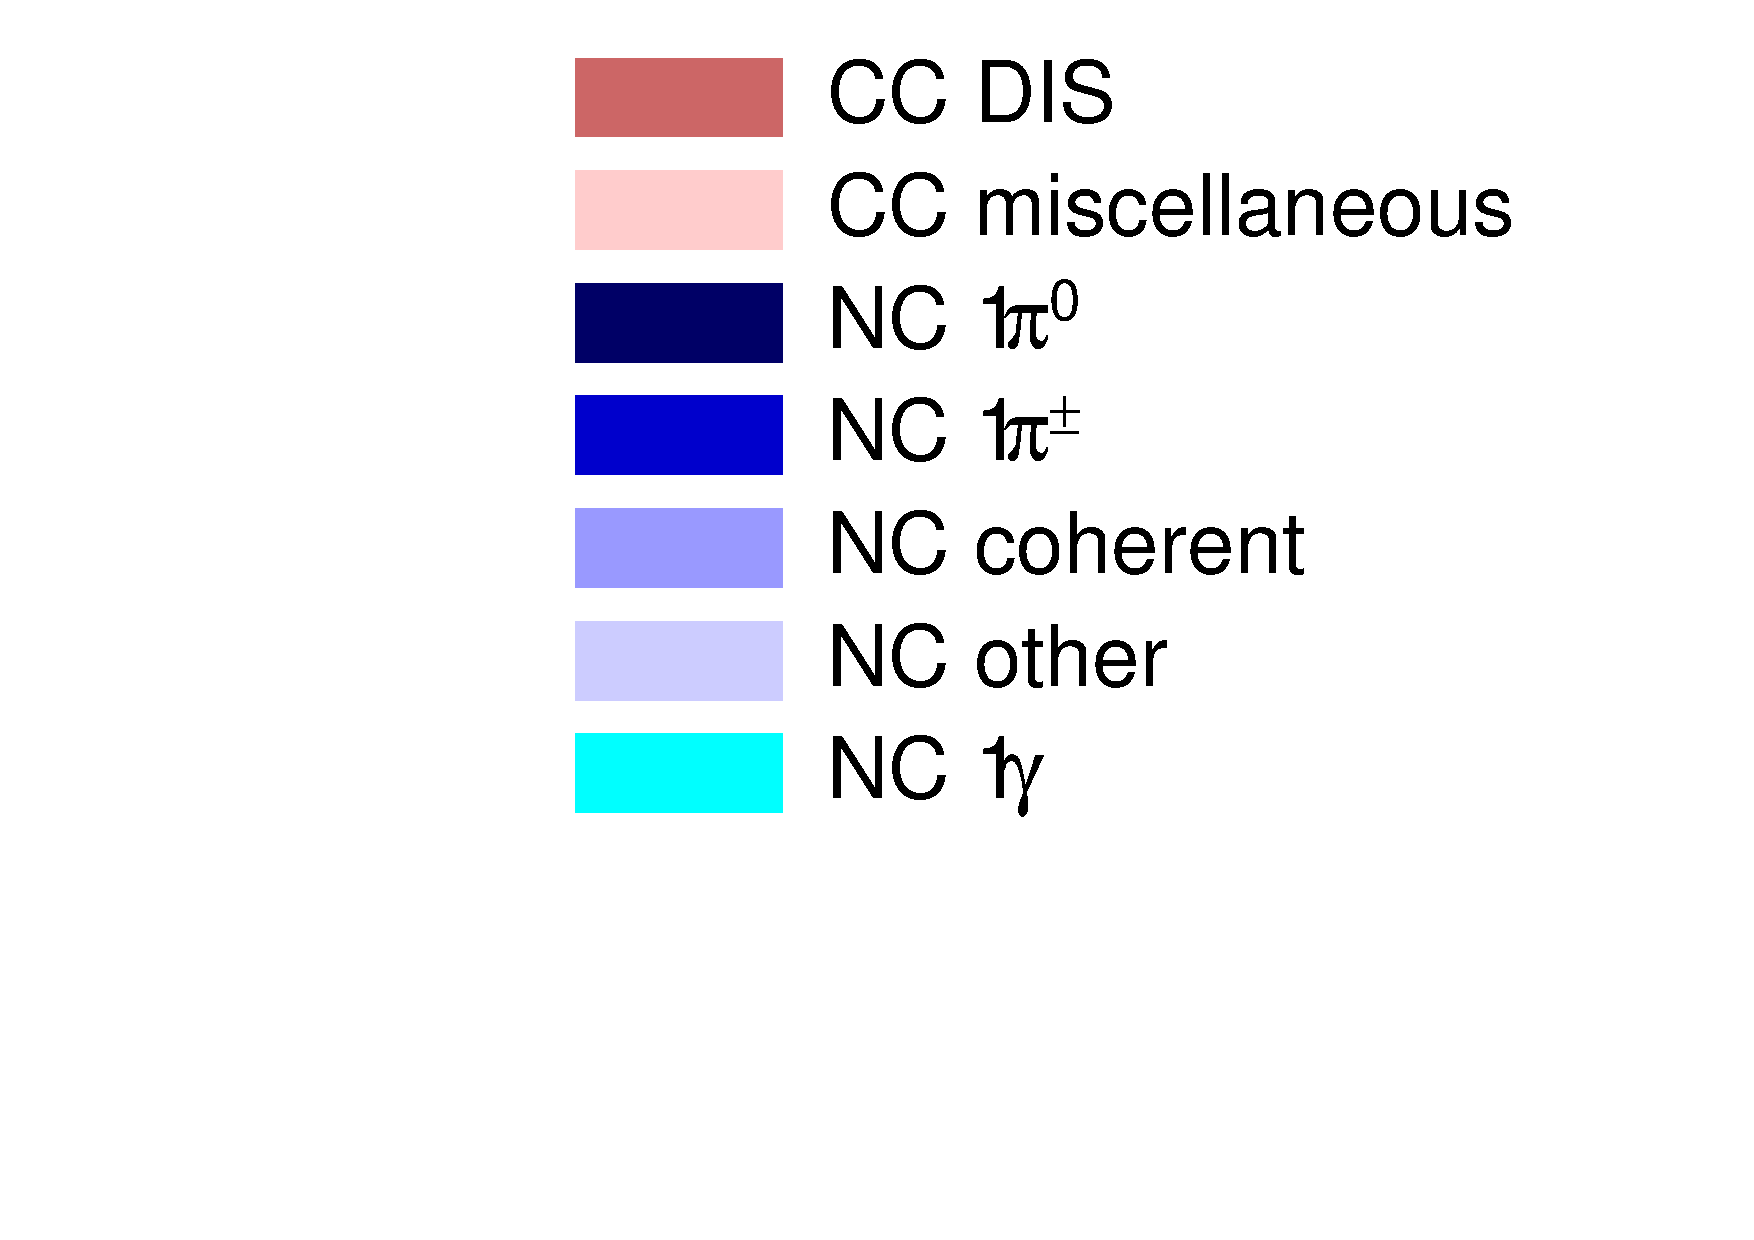
\includegraphics[width=0.7\linewidth]{figs/legend2}
\end{subfigure}
\begin{subfigure}{.32\textwidth}
  \centering
  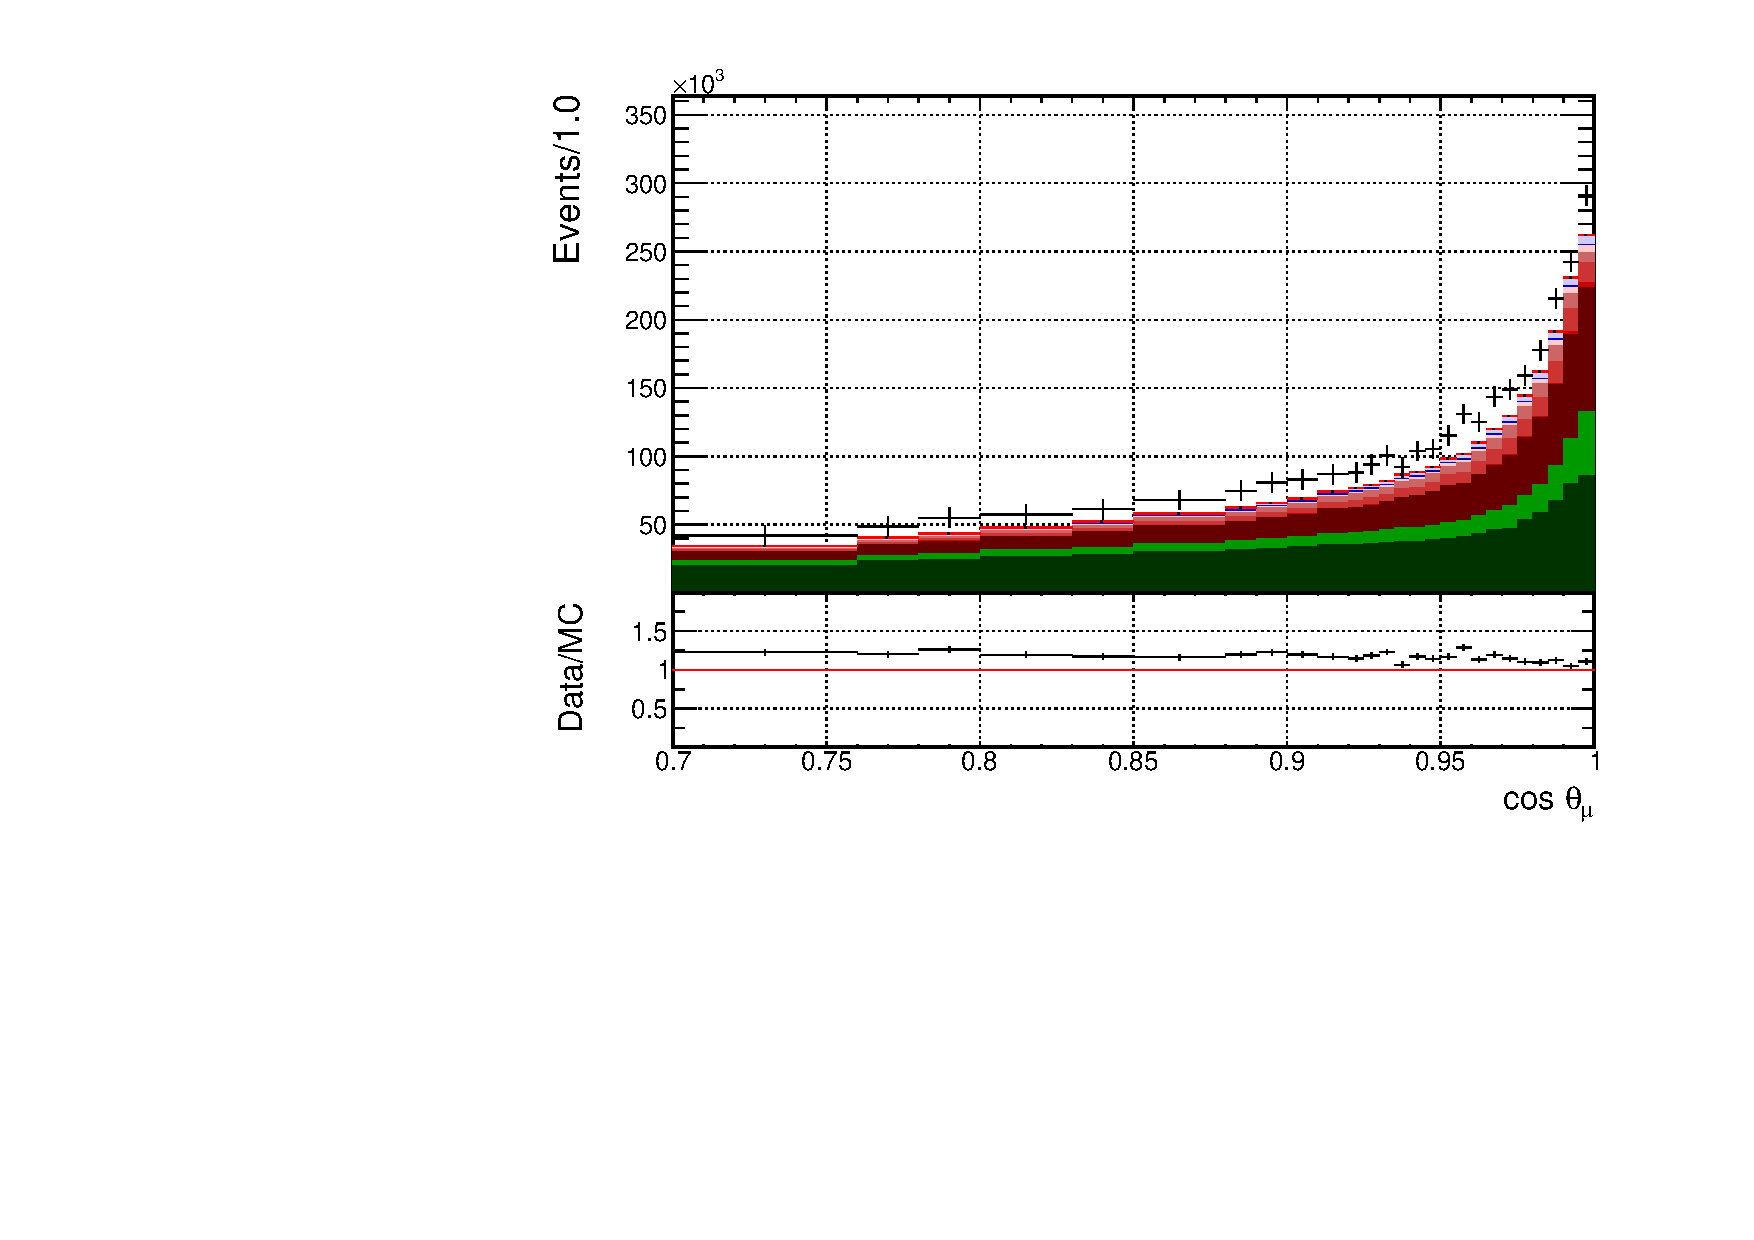
\includegraphics[width=0.95\linewidth]{figs/FGD1_numuCC_0pi_t}
  \caption{FGD1 FHC $\nu_{\mu}$ 0$\pi$}
  \label{fig:tstack_FGD1_numuCC_0pi}
\end{subfigure}
\begin{subfigure}{.32\textwidth}
  \centering
  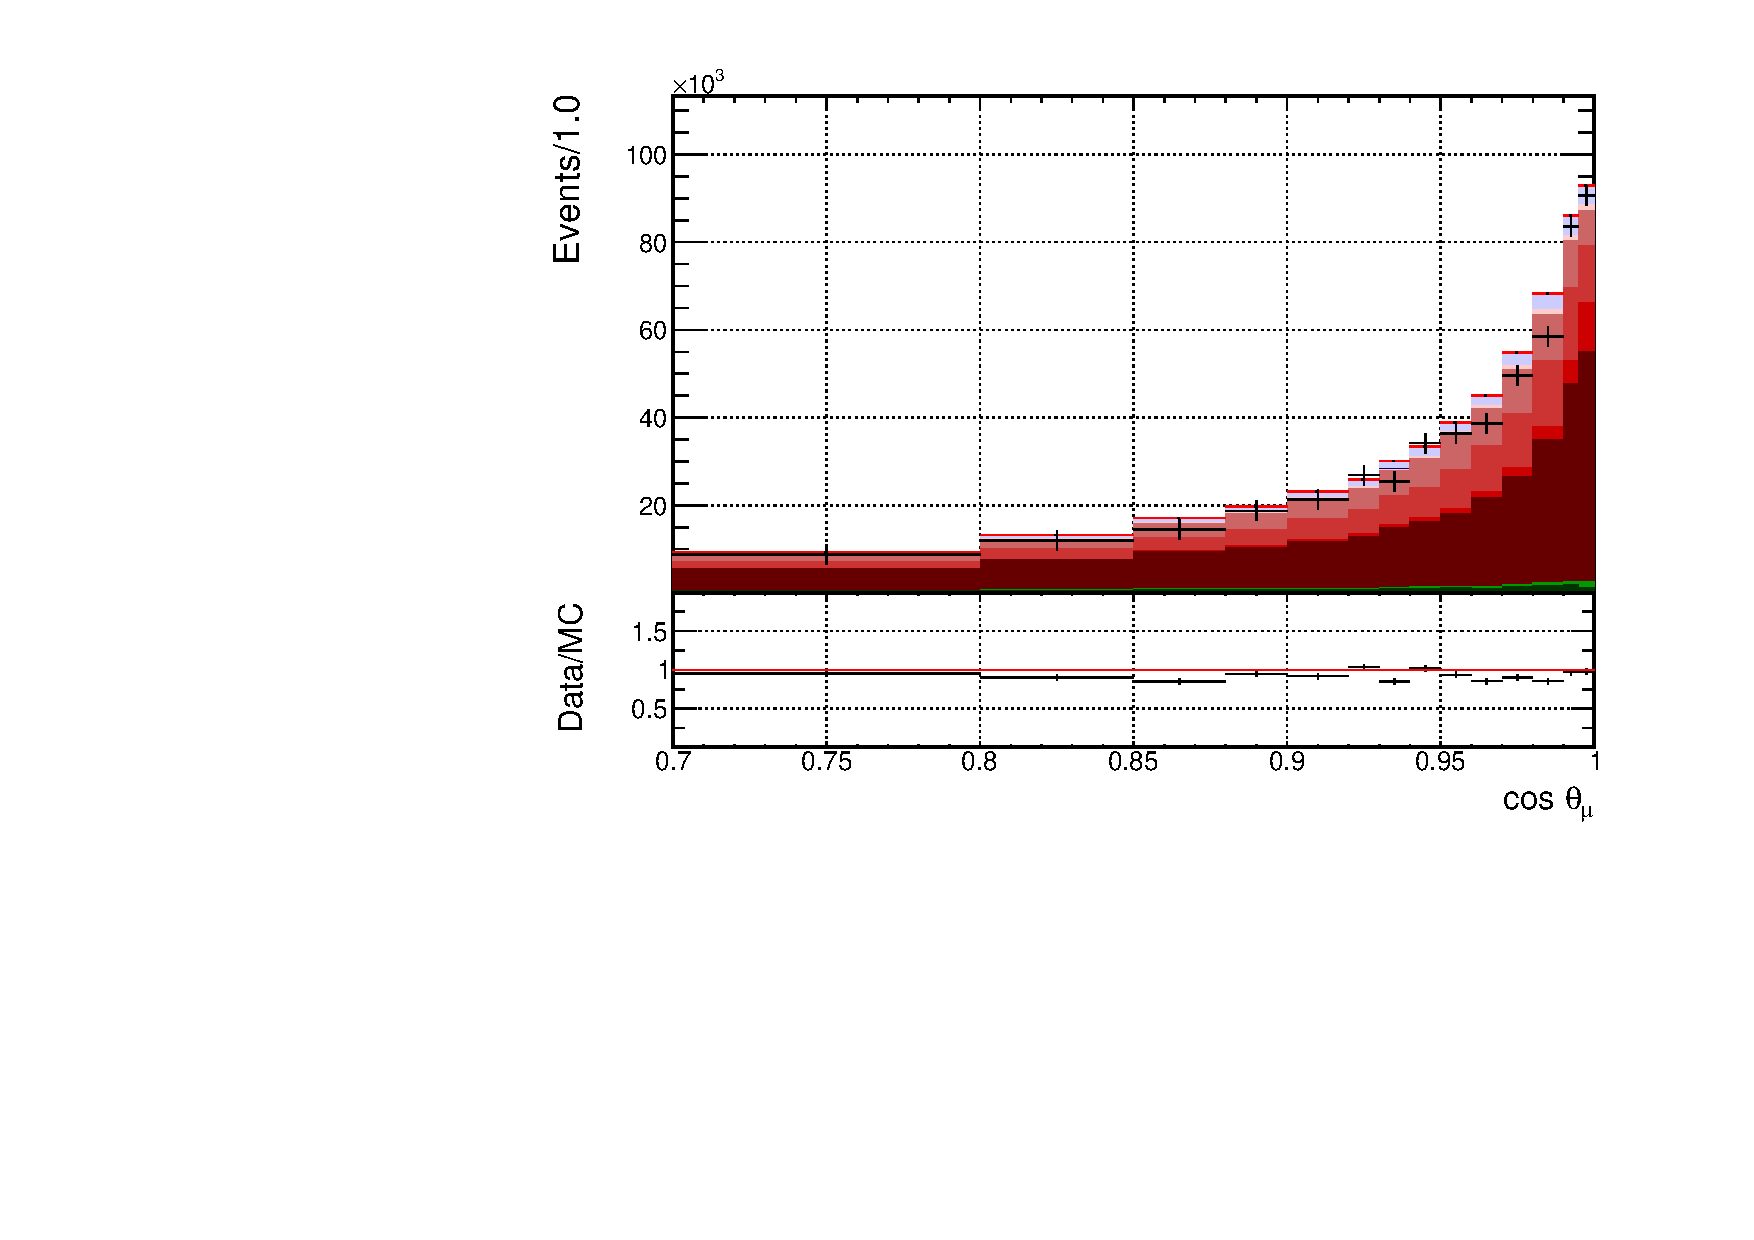
\includegraphics[width=0.95\linewidth]{figs/FGD1_numuCC_1pi_t}
  \caption{FGD1 FHC $\nu_{\mu}$ 1$\pi$}
  \label{fig:tstack_FGD1_numuCC_1pi}
\end{subfigure}
\begin{subfigure}{.32\textwidth}
  \centering
  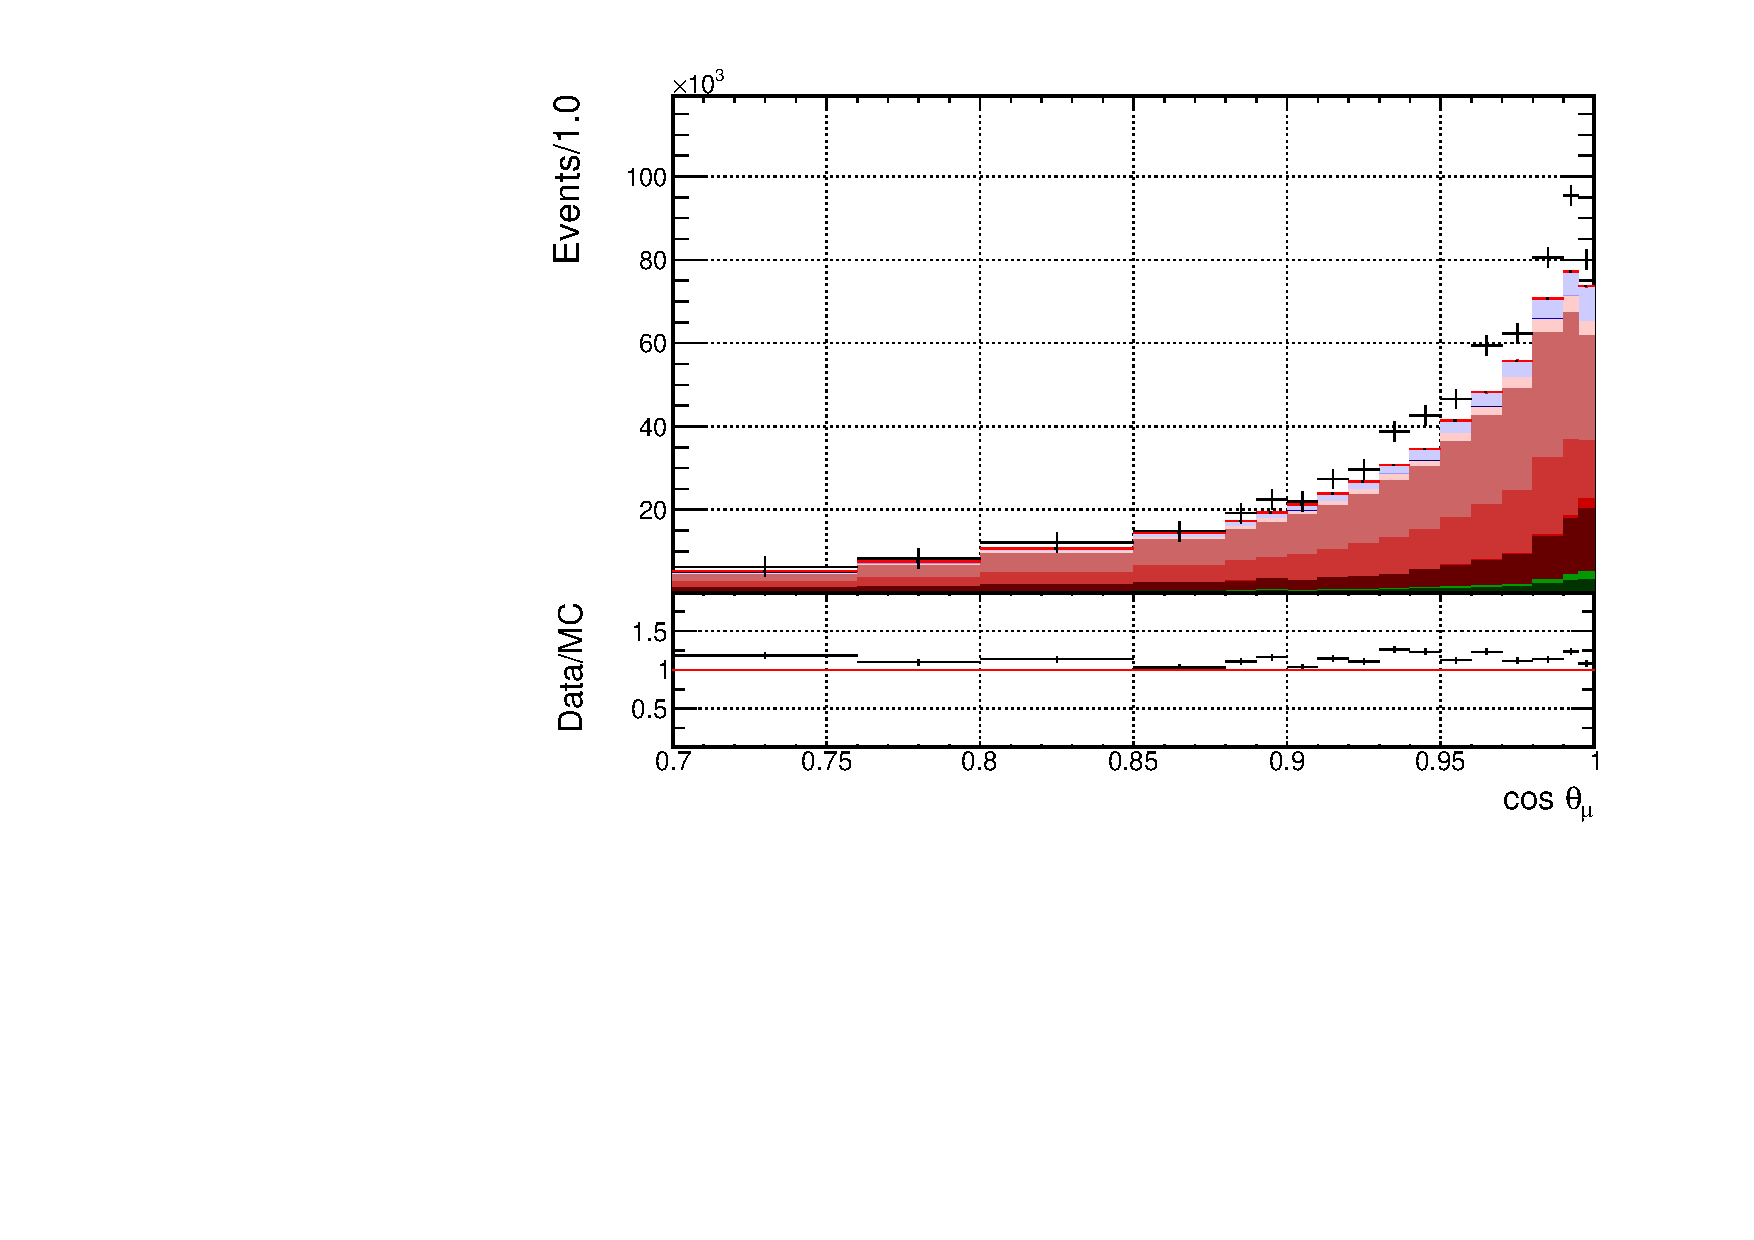
\includegraphics[width=0.95\linewidth]{figs/FGD1_numuCC_other_t}
  \caption{FGD1 FHC $\nu_{\mu}$ Other}
  \label{fig:tstack_FGD1_numuCC_other}
\end{subfigure}
\centering
\begin{subfigure}{.32\textwidth}
  \centering
  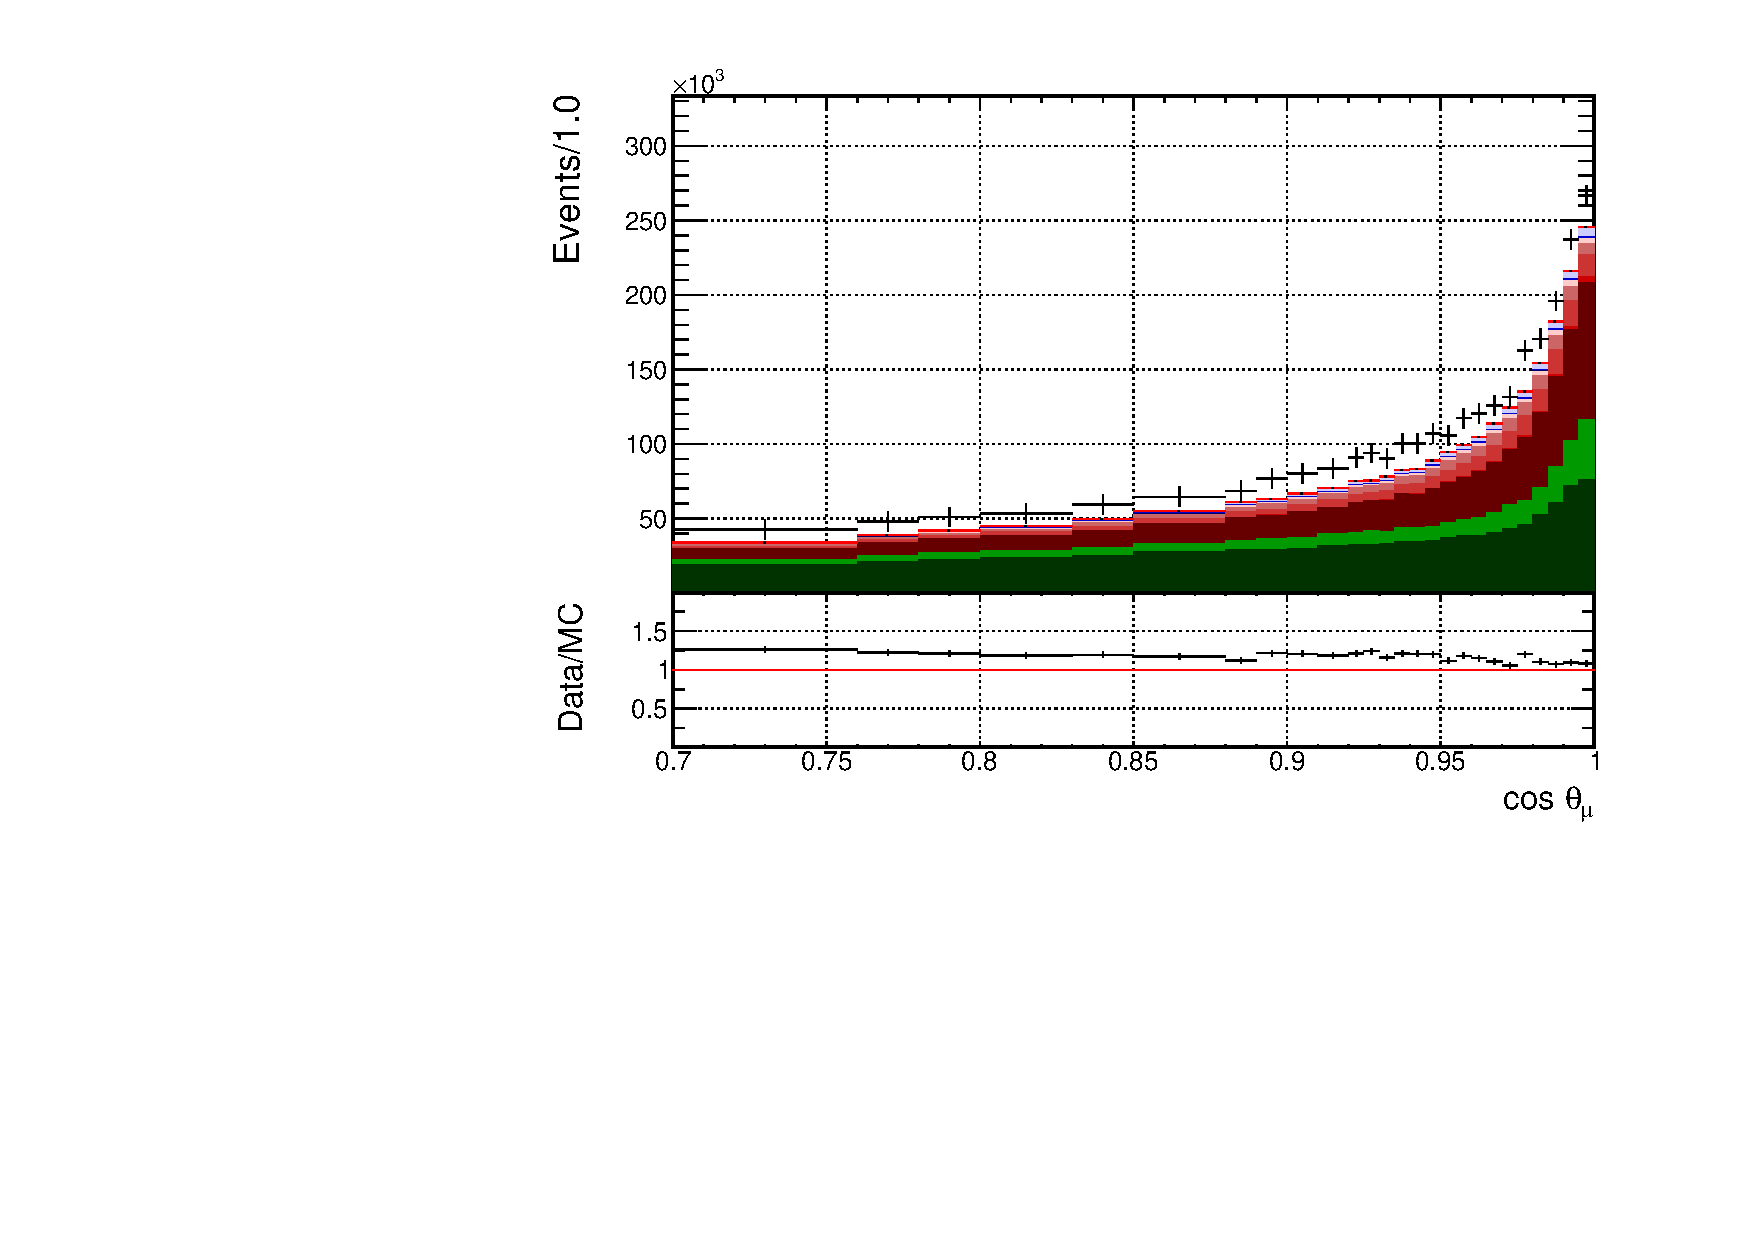
\includegraphics[width=0.95\linewidth]{figs/FGD2_numuCC_0pi_t}
  \caption{FGD2 FHC $\nu_{\mu}$ 0$\pi$}
  \label{fig:tstack_FGD2_numuCC_0pi}
\end{subfigure}
\begin{subfigure}{.32\textwidth}
  \centering
  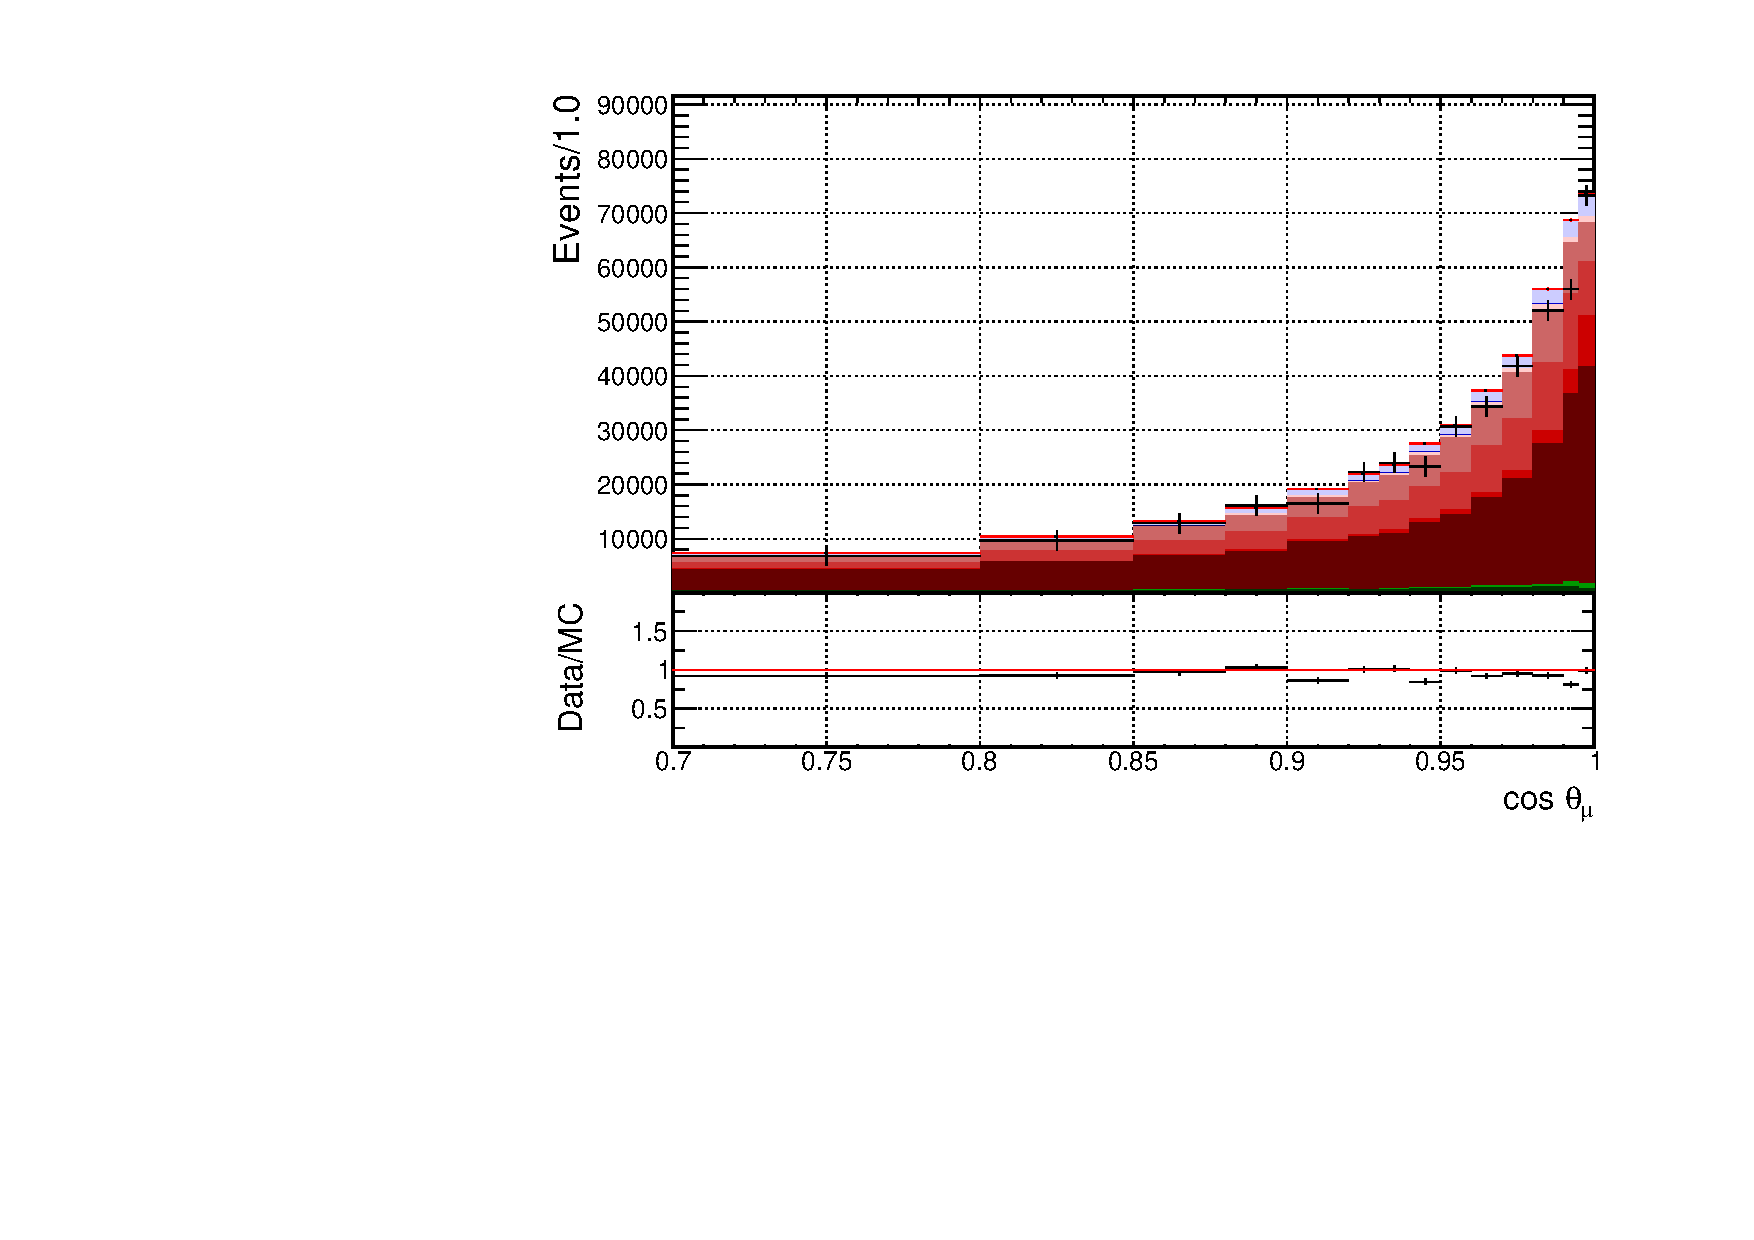
\includegraphics[width=0.95\linewidth]{figs/FGD2_numuCC_1pi_t}
  \caption{FGD2 FHC $\nu_{\mu}$ 1$\pi$}
  \label{fig:tstack_FGD2_numuCC_1pi}
\end{subfigure}
\begin{subfigure}{.32\textwidth}
  \centering
  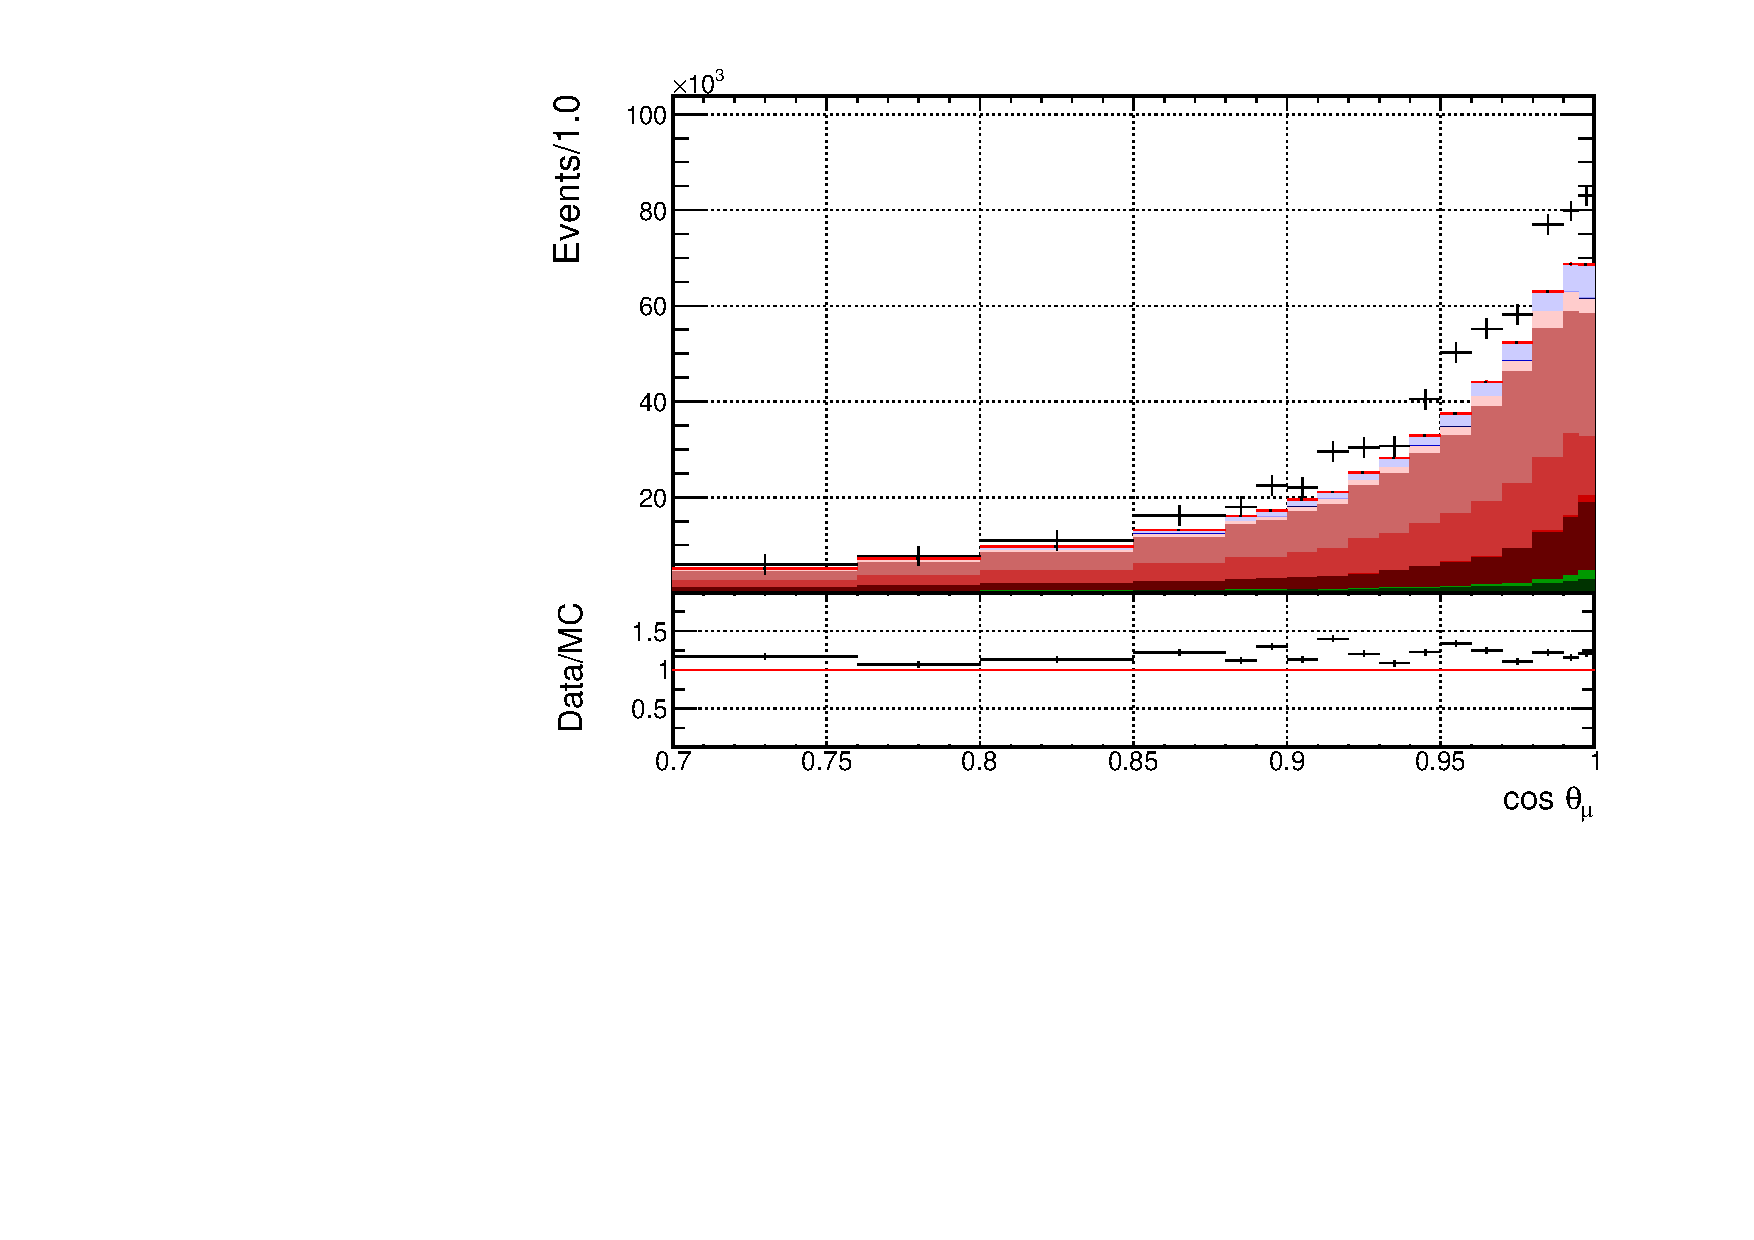
\includegraphics[width=0.95\linewidth]{figs/FGD2_numuCC_other_t}
  \caption{FGD2 $\nu_{\mu}$ Other}
  \label{fig:tstack_FGD2_numuCC_other}
\end{subfigure}
\centering
\begin{subfigure}{.32\textwidth}
  \centering
  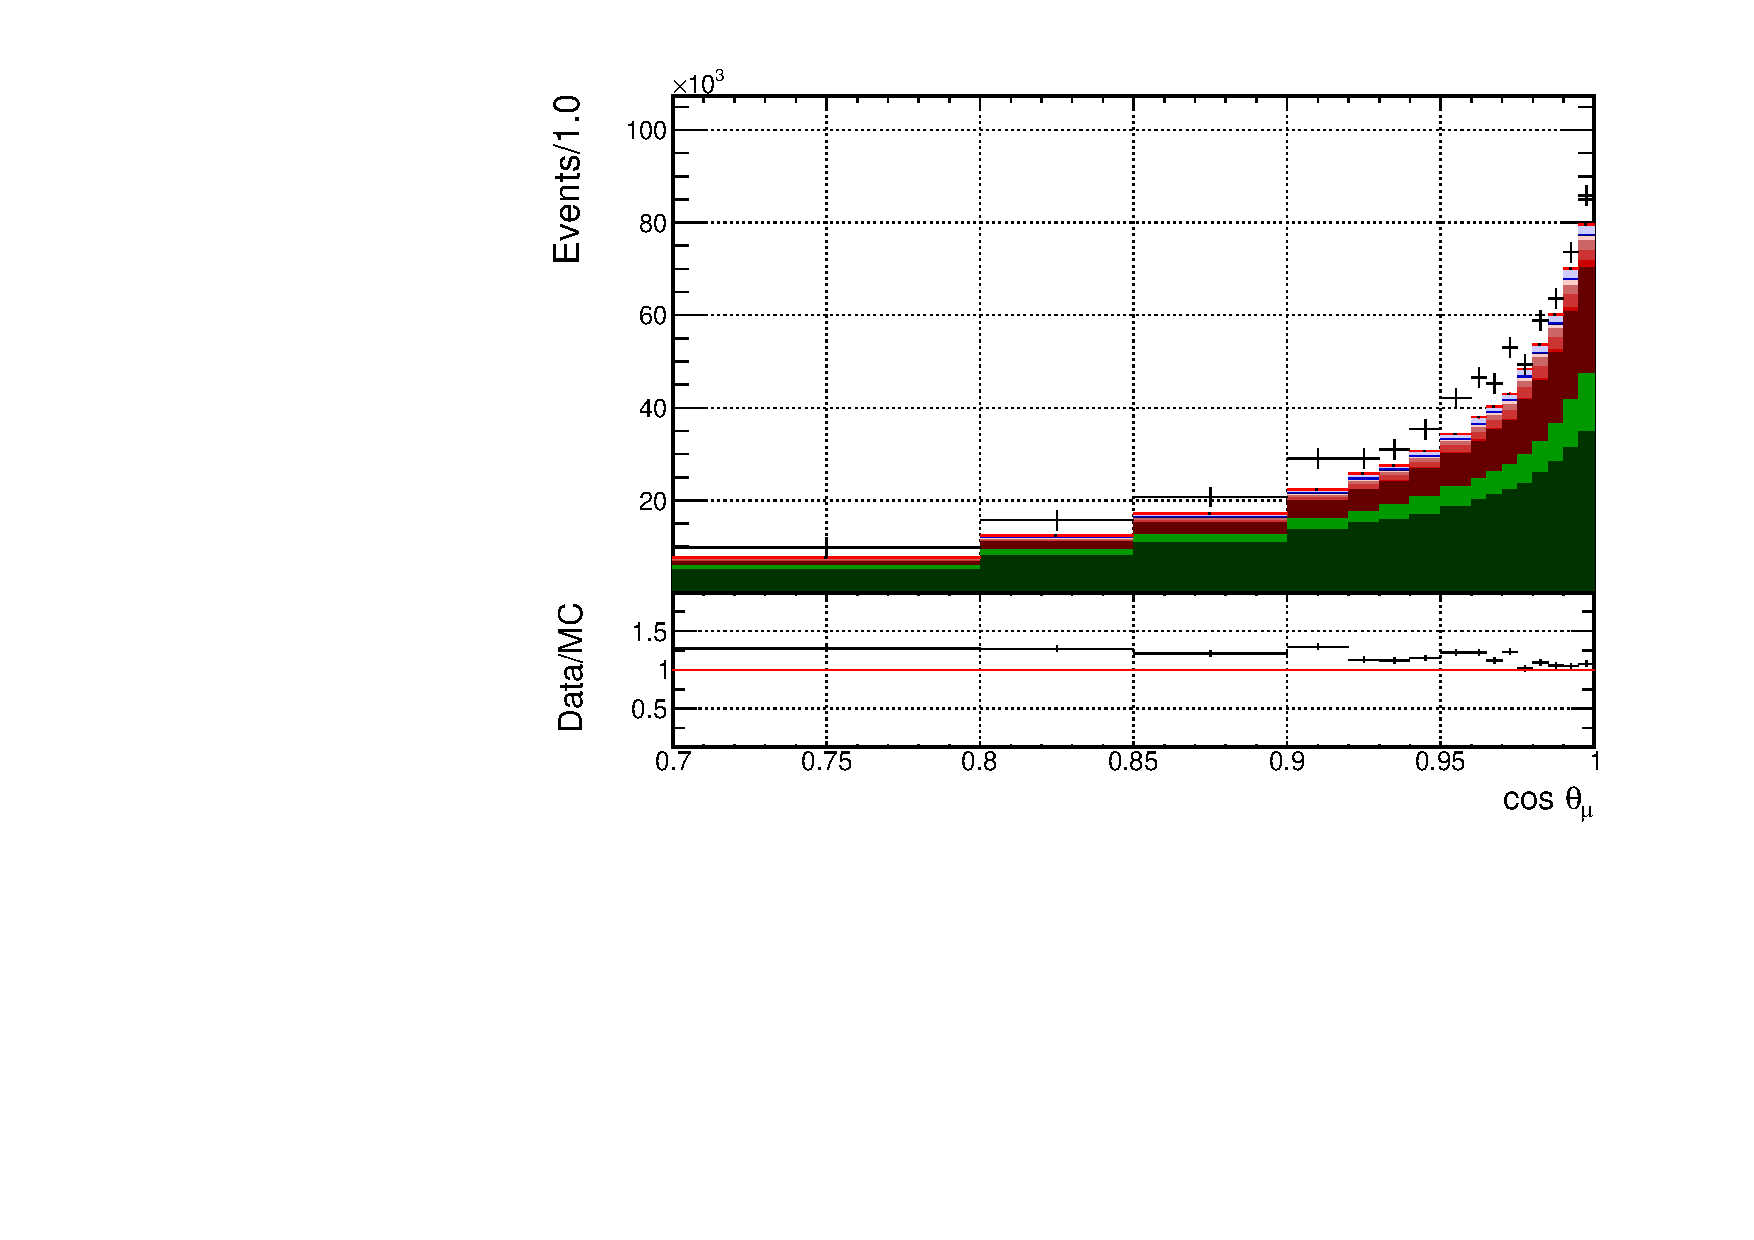
\includegraphics[width=0.95\linewidth]{figs/FGD1_anti-numuCC_0pi_t}
  \caption{FGD1 RHC $\bar{\nu_{\mu}}$ 0$\pi$}
  \label{fig:tstack_FGD1_anti-numuCC_0pi}
\end{subfigure}
\begin{subfigure}{.32\textwidth}
  \centering
  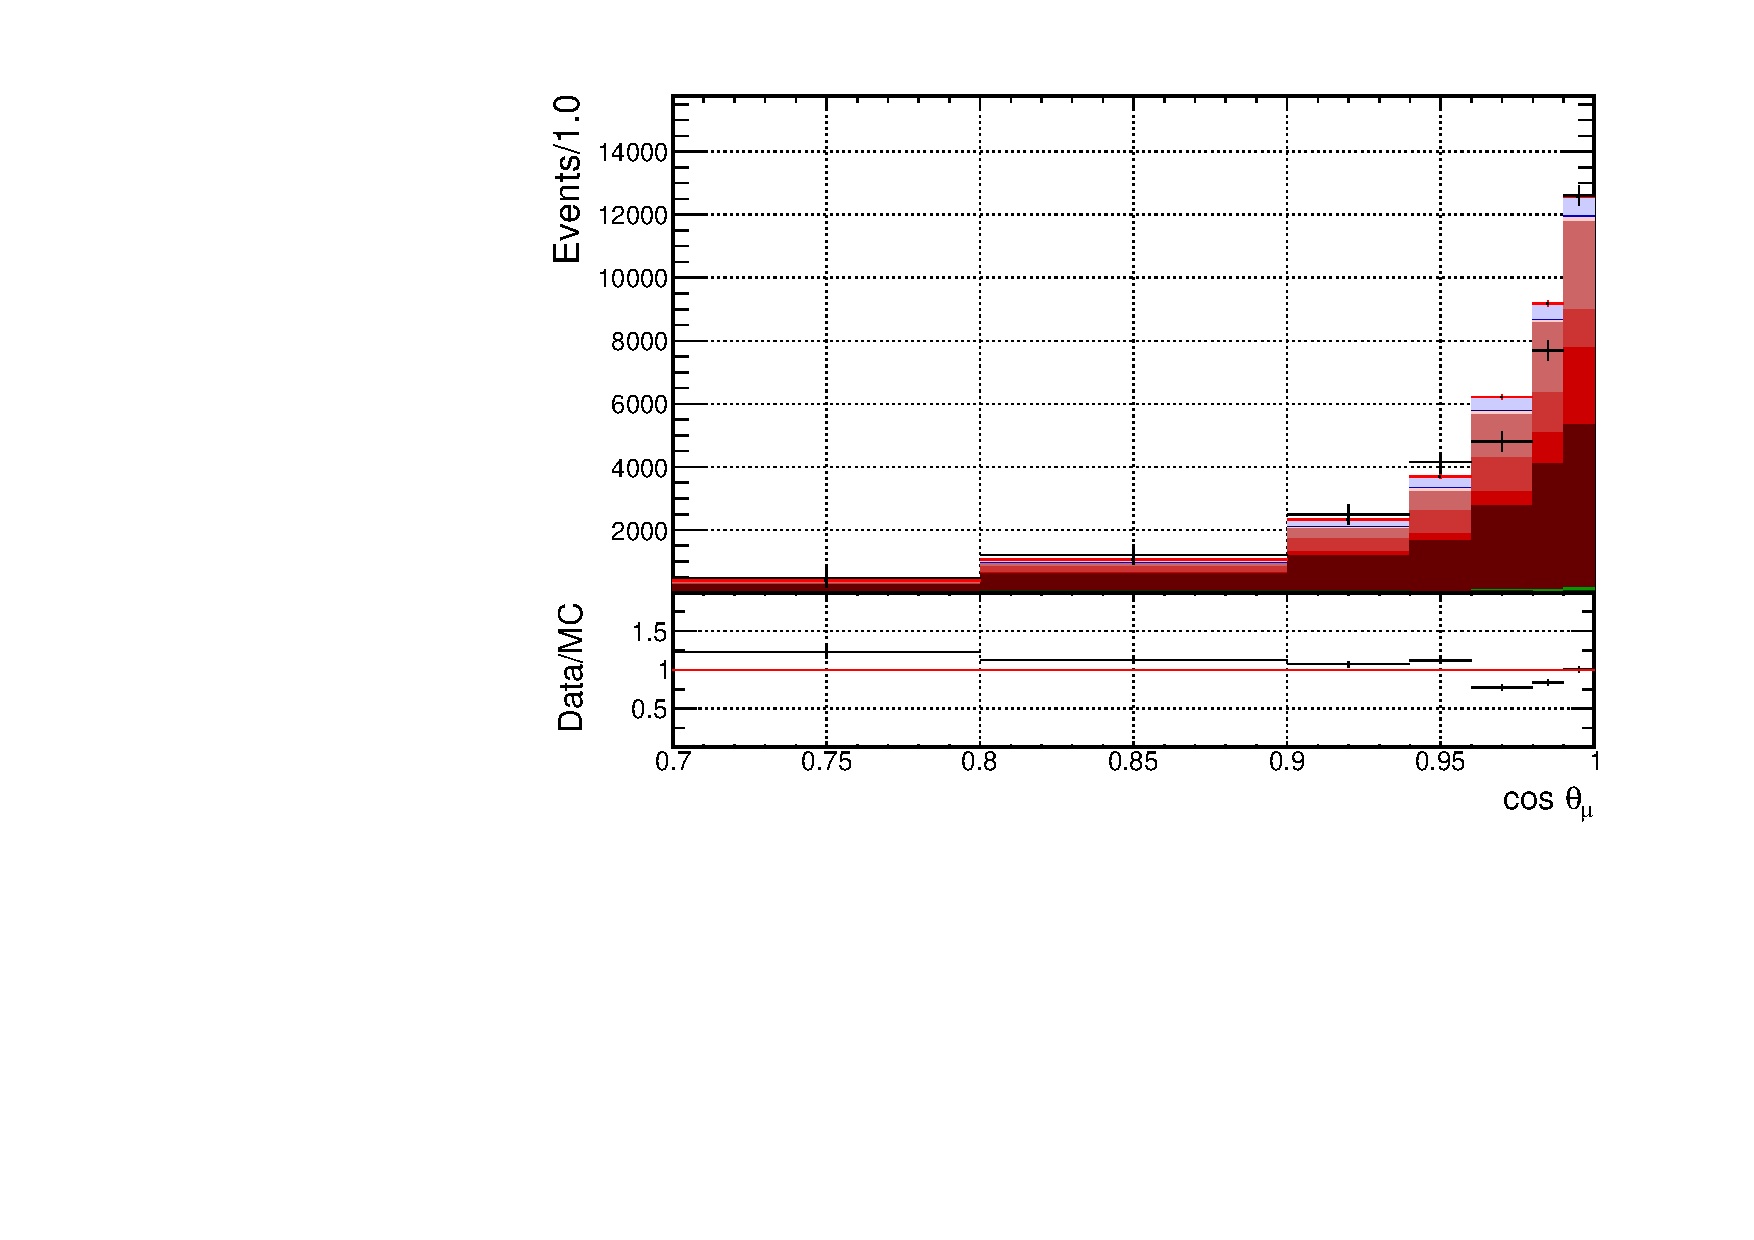
\includegraphics[width=0.95\linewidth]{figs/FGD1_anti-numuCC_1pi_t}
  \caption{FGD1 RHC $\bar{\nu_{\mu}}$ 1$\pi$}
  \label{fig:tstack_FGD1_anti-numuCC_1pi}
\end{subfigure}
\begin{subfigure}{.32\textwidth}
  \centering
  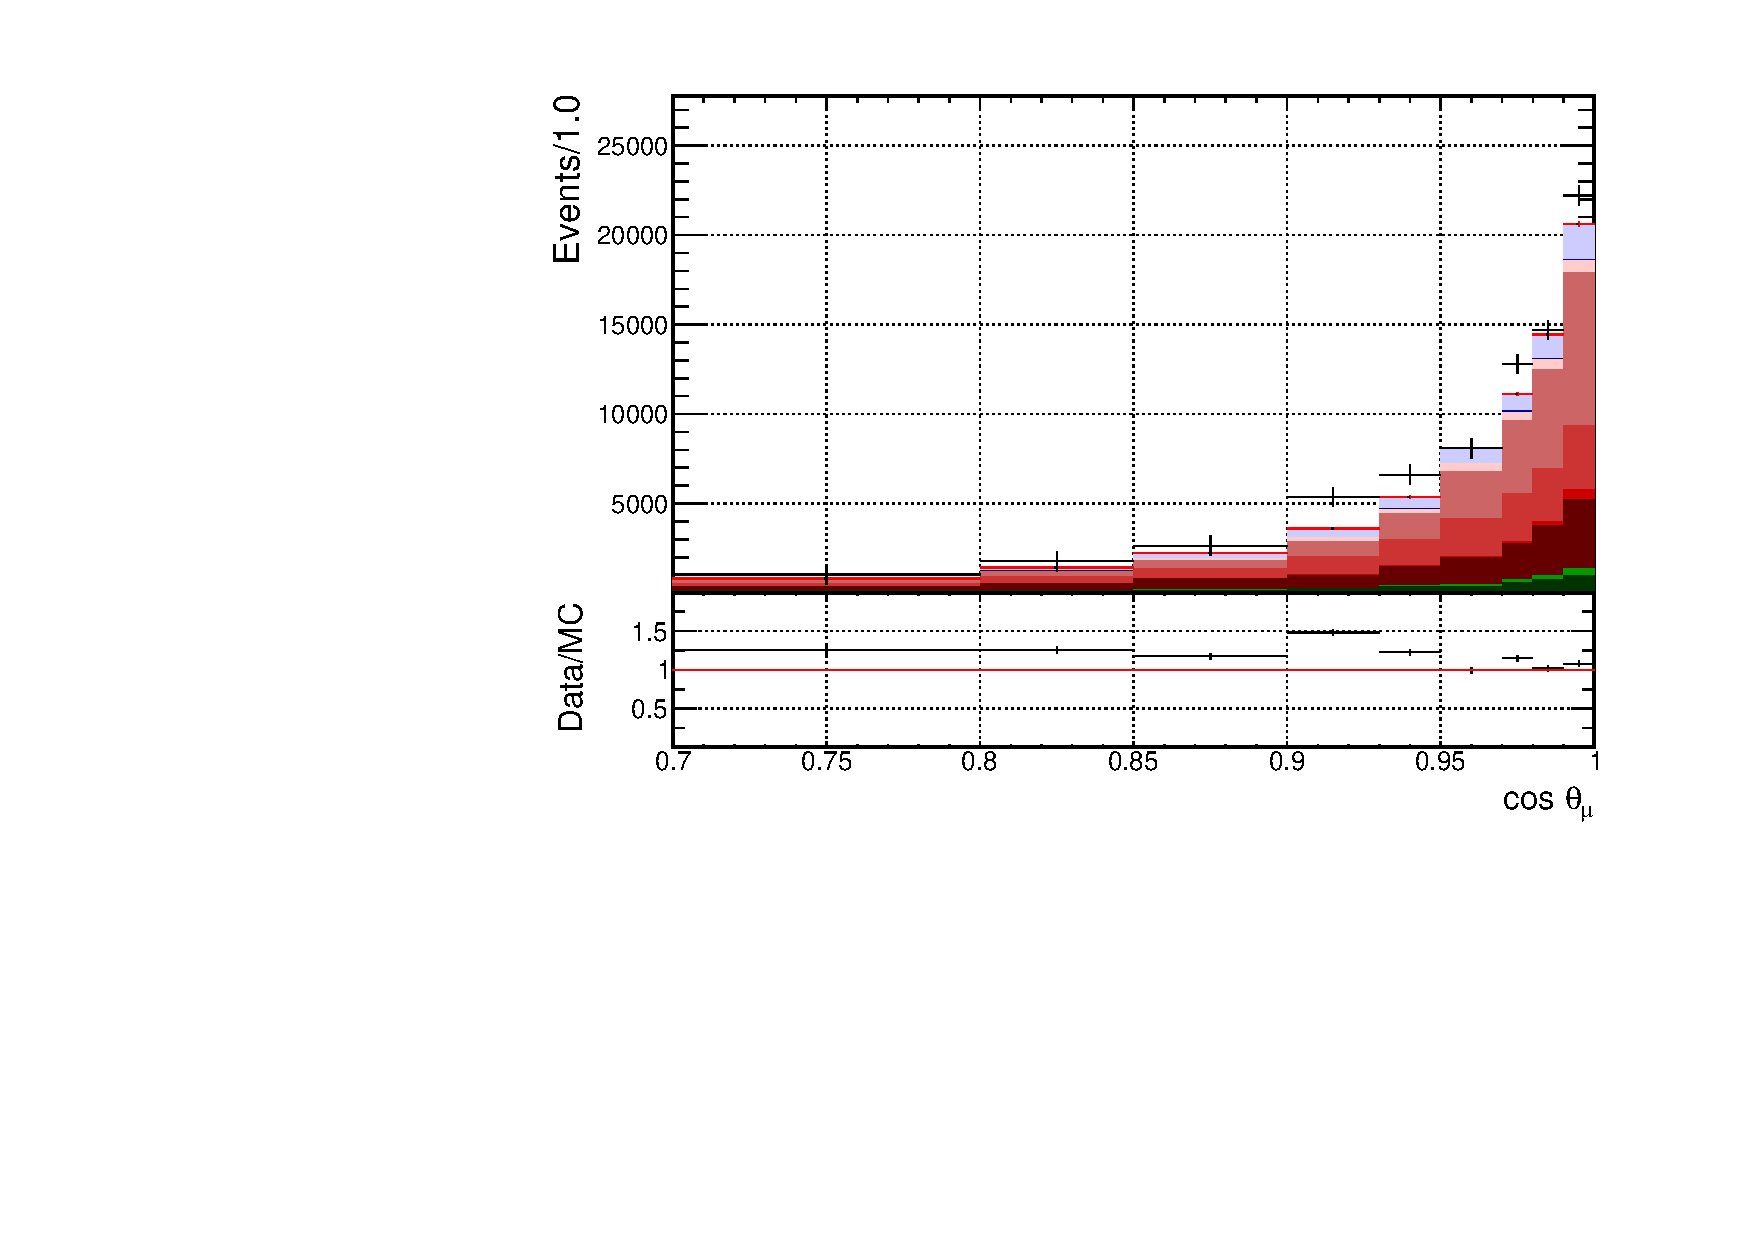
\includegraphics[width=0.95\linewidth]{figs/FGD1_anti-numuCC_other_t}
  \caption{FGD1 RHC $\bar{\nu_{\mu}}$ Other}
  \label{fig:tstack_FGD1_anti-numuCC_other}
\end{subfigure}
\centering
\begin{subfigure}{.32\textwidth}
  \centering
  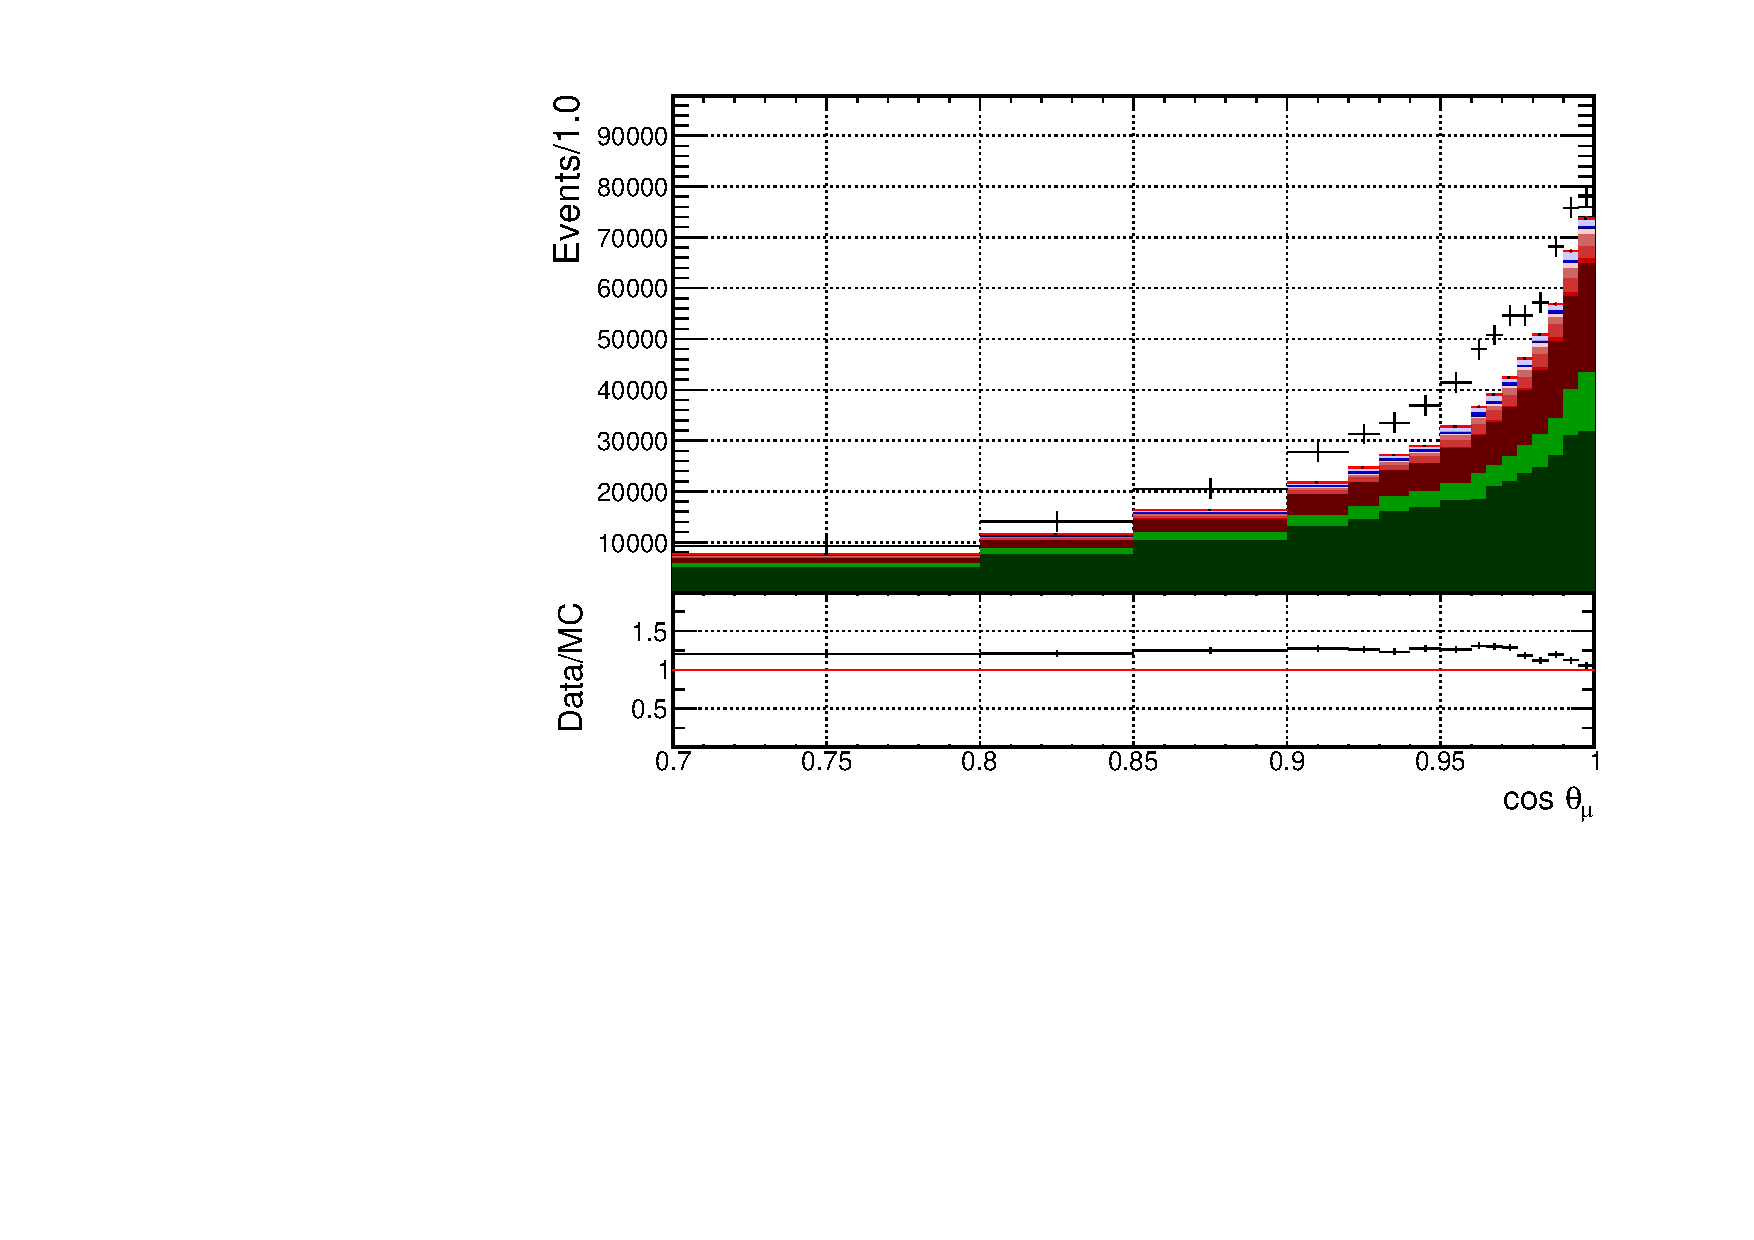
\includegraphics[width=0.95\linewidth]{figs/FGD2_anti-numuCC_0pi_t}
  \caption{FGD2 RHC $\bar{\nu_{\mu}}$ 0$\pi$}
  \label{fig:tstack_FGD2_anti-numuCC_0pi}
\end{subfigure}
\begin{subfigure}{.32\textwidth}
  \centering
  \includegraphics[width=0.95\linewidth]{figs/FGD2_anti-numuCC_1pi_t}
  \caption{FGD2 RHC $\bar{\nu_{\mu}}$ 1$\pi$}
  \label{fig:tstack_FGD2_anti-numuCC_1pi}
\end{subfigure}
\begin{subfigure}{.32\textwidth}
  \centering
  \includegraphics[width=0.95\linewidth]{figs/FGD2_anti-numuCC_other_t}
  \caption{FGD2 RHC $\bar{\nu_{\mu}}$ Other}
  \label{fig:tstack_FGD2_anti-numuCC_other}
\end{subfigure}
\begin{subfigure}{.32\textwidth}
  \centering
  \includegraphics[width=0.95\linewidth]{figs/FGD1_NuMuBkg_CC0pi_in_AntiNu_Mode_t}
  \caption{FGD1 RHC $\nu_{\mu}$ 0$\pi$}
  \label{fig:tstack_FGD1_NuMuBkg_CC0pi_in_AntiNu_Mode}
\end{subfigure}
\begin{subfigure}{.32\textwidth}
  \centering
  \includegraphics[width=0.95\linewidth]{figs/FGD1_NuMuBkg_CC1pi_in_AntiNu_Mode_t}
  \caption{FGD1 RHC $\nu_{\mu}$ 1$\pi$}
  \label{fig:tstack_FGD1_NuMuBkg_CC1pi_in_AntiNu_Mode}
\end{subfigure}
\begin{subfigure}{.32\textwidth}
  \centering
  \includegraphics[width=0.95\linewidth]{figs/FGD1_NuMuBkg_CCOther_in_AntiNu_Mode_t}
  \caption{FGD1 RHC $\nu_{\mu}$ Other}
  \label{fig:tstack_FGD1_NuMuBkg_CCOther_in_AntiNu_Mode}
\end{subfigure}
\begin{subfigure}{.32\textwidth}
  \centering
  \includegraphics[width=0.95\linewidth]{figs/FGD2_NuMuBkg_CC0pi_in_AntiNu_Mode_t}
  \caption{FGD2 RHC $\nu_{\mu}$ 0$\pi$}
  \label{fig:tstack_FGD2_NuMuBkg_CC0pi_in_AntiNu_Mode}
\end{subfigure}
\begin{subfigure}{.32\textwidth}
  \centering
  \includegraphics[width=0.95\linewidth]{figs/FGD2_NuMuBkg_CC1pi_in_AntiNu_Mode_t}
  \caption{FGD2 RHC $\nu_{\mu}$ 1$\pi$}
  \label{fig:tstack_FGD2_NuMuBkg_CC1pi_in_AntiNu_Mode}
\end{subfigure}
\begin{subfigure}{.32\textwidth}
  \centering
  \includegraphics[width=0.95\linewidth]{figs/FGD2_NuMuBkg_CCOther_in_AntiNu_Mode_t}
  \caption{FGD2 RHC $\nu_{\mu}$ Other}
  \label{fig:tstack_FGD2_NuMuBkg_CCOther_in_AntiNu_Mode}
\end{subfigure}
\caption{cos $\theta_{\mu}$ projections of data and nominal MC broken down by interaction mode.}
\label{fig:tstack}
\end{figure}

\section{Log Likelihood Scans}\label{sec:llhscan}

As described in Section \ref{sec:extrac}, the marginalisation effects from extracting correlated and non-Gaussian parameters from the full posterior distribution can cause the fit to appear biased. A full Asimov fit alone, described in Section \ref{sec:asimov}, is therefore not a good method of validating the framework. 

Log likelihood scans are therefore also run as part of the validations. The nominal MC is set as the data, and each systematic parameter is varied one at a time to 150 equally spaced points from -1$\sigma$ to +1$\sigma$. At each step, the MC is reweighted and the total likelihood from all contributions calculated. Only the diagonal terms of the covariance matrices are used for the penalty contribution, as otherwise varying one parameter alone could invoke significant penalties due to correlations. 
The scans are therefore not a fully accurate measure of the sensitivity of the fit to constrain each systematic, but a useful validation of the framework.

After each scan, the parameter is reset, and the next parameter in question varied. The likelihood response is expected to be fairly Gaussian for each parameter, as the prior uncertainty is either Gaussian or flat, and most parameters are expected to have a symmetric effect on the number of events in individual bins. The minimum should be at the prior central value of the parameter, and the log-likelihood here should be 0, as at this point the reweighted MC is identical to the nominal MC. No variation of a single parameter should be able to produce a set of distributions more similar to the nominal MC than itself.

The log likelihood scans for four selected interaction parameters are shown in Figure \ref{fig:llhxsec}. As expected, the test statistic minimises to 0 at the prior central value of each parameter. The penalty contribution to the log likelihood dominates for the CC normalisation parameter, due to the prior uncertainty being so small. Conversely, the 2p2h C to O normalisation parameter has a weaker prior and therefore a larger contribution from the sample likelihood. The likelihood for the $0.0 < Q^2 < 0.05$ GeV$^2$ normalisation parameter is entirely dominated by the sample contribution, as the prior is flat. The CC DIS and mult-$\pi \bar{\nu}$ normalisation parameter has more balanced contributions from both the sample and penalty likelihoods.

\begin{figure}
\centering
\begin{subfigure}{.49\textwidth}
  \centering
  \includegraphics[width=0.7\linewidth]{figs/llh/CC_norm_nu_llh.pdf}
  \caption{CC normalisation $\nu$}
\end{subfigure}
\begin{subfigure}{.49\textwidth}
  \centering
  \includegraphics[width=0.7\linewidth]{figs/llh/2p2h_normCtoO_llh.pdf}
  \caption{2p2h C to O normalisation}
\end{subfigure}
\begin{subfigure}{.49\textwidth}
  \centering
  \includegraphics[width=0.7\linewidth]{figs/llh/Q2_norm_1_llh.pdf}
  \caption{$0.0 < Q^2 < 0.05$ normalisation}
\end{subfigure}
\begin{subfigure}{.49\textwidth}
  \centering
  \includegraphics[width=0.7\linewidth]{figs/llh/CC_DIS_MultPi_Norm_Nubar_llh.pdf}
  \caption{CC DIS and mult-$\pi$ normalisation}
\end{subfigure}
\caption{Log likelihood scans for selected interaction parameters.}
\label{fig:llhxsec}
\end{figure}

The log likelihood scans for four selected flux parameters are shown in Figure \ref{fig:llhflux}. The test statistic again minimises to 0 at the prior central value of each parameter, as expected. These parameters all have tight prior uncertainties, and so the penalty terms dominate the likelihoods. For the SK flux parameters, there is no sample contribution to the likelihood. This is expected as the SK flux parameters should have no effect on the ND280 samples (apart from through the correlations with ND280 flux parameters, which are not included in these scans). 

\begin{figure}
\centering
\begin{subfigure}{.49\textwidth}
  \centering
  \includegraphics[width=0.7\linewidth]{figs/llh/b_5_llh.pdf}
  \caption{ND280 FHC $\nu_{\mu}$ 1-1.5 GeV}
\end{subfigure}
\begin{subfigure}{.49\textwidth}
  \centering
  \includegraphics[width=0.7\linewidth]{figs/llh/b_12_llh.pdf}
  \caption{ND280 FHC $\nu_{e}$ 0.5-0.7 GeV}
\end{subfigure}
\begin{subfigure}{.49\textwidth}
  \centering
  \includegraphics[width=0.7\linewidth]{figs/llh/b_36_llh.pdf}
  \caption{ND280 RHC $\nu_e$ 2.5-30 GeV}
\end{subfigure}
\begin{subfigure}{.49\textwidth}
  \centering
  \includegraphics[width=0.7\linewidth]{figs/llh/b_52_llh.pdf}
  \caption{SK RHC $\bar{\nu_{\mu}}$ 0.5-0.6 GeV}
\end{subfigure}
\caption{Log likelihood scans for selected flux parameters.}
\label{fig:llhflux}
\end{figure}

The log likelihood scans for four selected ND280 detector parameters are shown in Figure \ref{fig:llhdet}. As expected, the test statistics all minimise to 0 at the prior central value of each parameter. The prior dominates for all regions of $p_{\mu}$-cos $theta_{\mu}$in each sample. For the higher statistic regions (eg. FGD1 FHC $\nu_{\mu}$ CC 0$\pi$: 300-1000 MeV, 0.92-0.98), the overall constraint is larger than for the lower statistic regions, (eg. FGD1 FHC $\nu_{\mu}$ CC 1$\pi$: 5000-30000 MeV, -1.0-0.6). 

\begin{figure}
\centering
\begin{subfigure}{.49\textwidth}
  \centering
  \includegraphics[width=0.7\linewidth]{figs/llh/ndd_13_llh.pdf}
  \caption{FGD1 FHC $\nu_{\mu}$ CC 0$\pi$: 300-1000 MeV, 0.92-0.98}
\end{subfigure}
\begin{subfigure}{.49\textwidth}
  \centering
  \includegraphics[width=0.7\linewidth]{figs/llh/ndd_136_llh.pdf}
  \caption{FGD1 FHC $\nu_{\mu}$ CC 1$\pi$: 5000-30000 MeV, -1.0-0.6}
\end{subfigure}
\begin{subfigure}{.49\textwidth}
  \centering
  \includegraphics[width=0.7\linewidth]{figs/llh/ndd_541_llh.pdf}
  \caption{FGD2 RHC $\bar{\nu_{\mu}}$ CC Other: 800-30000 MeV, 0.97-1.0}
\end{subfigure}
\begin{subfigure}{.49\textwidth}
  \centering
  \includegraphics[width=0.7\linewidth]{figs/llh/ndd_556_llh.pdf}
  \caption{FGD1 RHC $\nu_{\mu}$ CC Other: 600-30000 MeV, -1.0-0.7}
\end{subfigure}
\caption{Log likelihood scans for selected ND280 detector parameters.}
\label{fig:llhdet}
\end{figure}

\section{Parameter Variations}\label{sec:sigvar}

As a further validation of the fitting framework and models, the parameters are again each set to $\pm1\sigma$, one by one, while all others are held at nominal. Instead of the change in likelihood, here the effect on the event distributions in $p_{\mu}$-cos$\theta_{\mu}$ is inspected. 

One varied interaction parameter for each sample is shown in Figure \ref{}. The combinations of parameter and sample were selected such that the parameter controls interactions targeted by the sample. The parameter in question is set to $+1\sigma$ above its nominal value, and the ration of the nominal MC to the reweighted MC is taken

%describe some of the distributions + make the plots

The total number of events in each sample at each variation is compared between the near detector fitting groups to verify that each parameter is behaving in the same way in each framework. .

\section{Asimov Fit}\label{sec:asimov}
%describe process
% fit results
%covariance matrix

\section{Data Fit}\label{sec:datafit}
%results
%cov
\section{Posterior Predictions}\label{sec:postpred}
%distributions in 1D? need script
%data, nom mc, fitted mc rates
%p value plots + table
%LLH dists
%SK PP need files and script

\section{Finer Fit and Detector Binning}\label{sec:newbin}
%New fit binning distributions
%say new detector binning is fit binning
\subsection{Asimov Fits}
%Fit results (poly both, th2d both, poly+574, th2d+574(which is orig)
%cov *3
\subsection{Data Fits}
%Fit results * 4
%tab data, nom mc, fitted mc rates*3
%cov * 3
\subsection{Posterior Predictions}
%distributions in 1D?*3
%pvalue table of all 4
%LLH conts (*3, or just polyboth?)
%SK PP all
\section{Oscillation Parameter Sensitivity}

\newpage
